% Options for packages loaded elsewhere
\PassOptionsToPackage{unicode}{hyperref}
\PassOptionsToPackage{hyphens}{url}
\PassOptionsToPackage{dvipsnames,svgnames,x11names}{xcolor}
%
\documentclass[
  letterpaper,
  DIV=11,
  numbers=noendperiod]{scrreprt}

\usepackage{amsmath,amssymb}
\usepackage{iftex}
\ifPDFTeX
  \usepackage[T1]{fontenc}
  \usepackage[utf8]{inputenc}
  \usepackage{textcomp} % provide euro and other symbols
\else % if luatex or xetex
  \usepackage{unicode-math}
  \defaultfontfeatures{Scale=MatchLowercase}
  \defaultfontfeatures[\rmfamily]{Ligatures=TeX,Scale=1}
\fi
\usepackage{lmodern}
\ifPDFTeX\else  
    % xetex/luatex font selection
\fi
% Use upquote if available, for straight quotes in verbatim environments
\IfFileExists{upquote.sty}{\usepackage{upquote}}{}
\IfFileExists{microtype.sty}{% use microtype if available
  \usepackage[]{microtype}
  \UseMicrotypeSet[protrusion]{basicmath} % disable protrusion for tt fonts
}{}
\makeatletter
\@ifundefined{KOMAClassName}{% if non-KOMA class
  \IfFileExists{parskip.sty}{%
    \usepackage{parskip}
  }{% else
    \setlength{\parindent}{0pt}
    \setlength{\parskip}{6pt plus 2pt minus 1pt}}
}{% if KOMA class
  \KOMAoptions{parskip=half}}
\makeatother
\usepackage{xcolor}
\setlength{\emergencystretch}{3em} % prevent overfull lines
\setcounter{secnumdepth}{5}
% Make \paragraph and \subparagraph free-standing
\ifx\paragraph\undefined\else
  \let\oldparagraph\paragraph
  \renewcommand{\paragraph}[1]{\oldparagraph{#1}\mbox{}}
\fi
\ifx\subparagraph\undefined\else
  \let\oldsubparagraph\subparagraph
  \renewcommand{\subparagraph}[1]{\oldsubparagraph{#1}\mbox{}}
\fi

\usepackage{color}
\usepackage{fancyvrb}
\newcommand{\VerbBar}{|}
\newcommand{\VERB}{\Verb[commandchars=\\\{\}]}
\DefineVerbatimEnvironment{Highlighting}{Verbatim}{commandchars=\\\{\}}
% Add ',fontsize=\small' for more characters per line
\usepackage{framed}
\definecolor{shadecolor}{RGB}{241,243,245}
\newenvironment{Shaded}{\begin{snugshade}}{\end{snugshade}}
\newcommand{\AlertTok}[1]{\textcolor[rgb]{0.68,0.00,0.00}{#1}}
\newcommand{\AnnotationTok}[1]{\textcolor[rgb]{0.37,0.37,0.37}{#1}}
\newcommand{\AttributeTok}[1]{\textcolor[rgb]{0.40,0.45,0.13}{#1}}
\newcommand{\BaseNTok}[1]{\textcolor[rgb]{0.68,0.00,0.00}{#1}}
\newcommand{\BuiltInTok}[1]{\textcolor[rgb]{0.00,0.23,0.31}{#1}}
\newcommand{\CharTok}[1]{\textcolor[rgb]{0.13,0.47,0.30}{#1}}
\newcommand{\CommentTok}[1]{\textcolor[rgb]{0.37,0.37,0.37}{#1}}
\newcommand{\CommentVarTok}[1]{\textcolor[rgb]{0.37,0.37,0.37}{\textit{#1}}}
\newcommand{\ConstantTok}[1]{\textcolor[rgb]{0.56,0.35,0.01}{#1}}
\newcommand{\ControlFlowTok}[1]{\textcolor[rgb]{0.00,0.23,0.31}{#1}}
\newcommand{\DataTypeTok}[1]{\textcolor[rgb]{0.68,0.00,0.00}{#1}}
\newcommand{\DecValTok}[1]{\textcolor[rgb]{0.68,0.00,0.00}{#1}}
\newcommand{\DocumentationTok}[1]{\textcolor[rgb]{0.37,0.37,0.37}{\textit{#1}}}
\newcommand{\ErrorTok}[1]{\textcolor[rgb]{0.68,0.00,0.00}{#1}}
\newcommand{\ExtensionTok}[1]{\textcolor[rgb]{0.00,0.23,0.31}{#1}}
\newcommand{\FloatTok}[1]{\textcolor[rgb]{0.68,0.00,0.00}{#1}}
\newcommand{\FunctionTok}[1]{\textcolor[rgb]{0.28,0.35,0.67}{#1}}
\newcommand{\ImportTok}[1]{\textcolor[rgb]{0.00,0.46,0.62}{#1}}
\newcommand{\InformationTok}[1]{\textcolor[rgb]{0.37,0.37,0.37}{#1}}
\newcommand{\KeywordTok}[1]{\textcolor[rgb]{0.00,0.23,0.31}{#1}}
\newcommand{\NormalTok}[1]{\textcolor[rgb]{0.00,0.23,0.31}{#1}}
\newcommand{\OperatorTok}[1]{\textcolor[rgb]{0.37,0.37,0.37}{#1}}
\newcommand{\OtherTok}[1]{\textcolor[rgb]{0.00,0.23,0.31}{#1}}
\newcommand{\PreprocessorTok}[1]{\textcolor[rgb]{0.68,0.00,0.00}{#1}}
\newcommand{\RegionMarkerTok}[1]{\textcolor[rgb]{0.00,0.23,0.31}{#1}}
\newcommand{\SpecialCharTok}[1]{\textcolor[rgb]{0.37,0.37,0.37}{#1}}
\newcommand{\SpecialStringTok}[1]{\textcolor[rgb]{0.13,0.47,0.30}{#1}}
\newcommand{\StringTok}[1]{\textcolor[rgb]{0.13,0.47,0.30}{#1}}
\newcommand{\VariableTok}[1]{\textcolor[rgb]{0.07,0.07,0.07}{#1}}
\newcommand{\VerbatimStringTok}[1]{\textcolor[rgb]{0.13,0.47,0.30}{#1}}
\newcommand{\WarningTok}[1]{\textcolor[rgb]{0.37,0.37,0.37}{\textit{#1}}}

\providecommand{\tightlist}{%
  \setlength{\itemsep}{0pt}\setlength{\parskip}{0pt}}\usepackage{longtable,booktabs,array}
\usepackage{calc} % for calculating minipage widths
% Correct order of tables after \paragraph or \subparagraph
\usepackage{etoolbox}
\makeatletter
\patchcmd\longtable{\par}{\if@noskipsec\mbox{}\fi\par}{}{}
\makeatother
% Allow footnotes in longtable head/foot
\IfFileExists{footnotehyper.sty}{\usepackage{footnotehyper}}{\usepackage{footnote}}
\makesavenoteenv{longtable}
\usepackage{graphicx}
\makeatletter
\def\maxwidth{\ifdim\Gin@nat@width>\linewidth\linewidth\else\Gin@nat@width\fi}
\def\maxheight{\ifdim\Gin@nat@height>\textheight\textheight\else\Gin@nat@height\fi}
\makeatother
% Scale images if necessary, so that they will not overflow the page
% margins by default, and it is still possible to overwrite the defaults
% using explicit options in \includegraphics[width, height, ...]{}
\setkeys{Gin}{width=\maxwidth,height=\maxheight,keepaspectratio}
% Set default figure placement to htbp
\makeatletter
\def\fps@figure{htbp}
\makeatother

\KOMAoption{captions}{tableheading}
\makeatletter
\makeatother
\makeatletter
\@ifpackageloaded{bookmark}{}{\usepackage{bookmark}}
\makeatother
\makeatletter
\@ifpackageloaded{caption}{}{\usepackage{caption}}
\AtBeginDocument{%
\ifdefined\contentsname
  \renewcommand*\contentsname{Table of contents}
\else
  \newcommand\contentsname{Table of contents}
\fi
\ifdefined\listfigurename
  \renewcommand*\listfigurename{List of Figures}
\else
  \newcommand\listfigurename{List of Figures}
\fi
\ifdefined\listtablename
  \renewcommand*\listtablename{List of Tables}
\else
  \newcommand\listtablename{List of Tables}
\fi
\ifdefined\figurename
  \renewcommand*\figurename{Figure}
\else
  \newcommand\figurename{Figure}
\fi
\ifdefined\tablename
  \renewcommand*\tablename{Table}
\else
  \newcommand\tablename{Table}
\fi
}
\@ifpackageloaded{float}{}{\usepackage{float}}
\floatstyle{ruled}
\@ifundefined{c@chapter}{\newfloat{codelisting}{h}{lop}}{\newfloat{codelisting}{h}{lop}[chapter]}
\floatname{codelisting}{Listing}
\newcommand*\listoflistings{\listof{codelisting}{List of Listings}}
\makeatother
\makeatletter
\@ifpackageloaded{caption}{}{\usepackage{caption}}
\@ifpackageloaded{subcaption}{}{\usepackage{subcaption}}
\makeatother
\makeatletter
\@ifpackageloaded{tcolorbox}{}{\usepackage[skins,breakable]{tcolorbox}}
\makeatother
\makeatletter
\@ifundefined{shadecolor}{\definecolor{shadecolor}{rgb}{.97, .97, .97}}
\makeatother
\makeatletter
\makeatother
\makeatletter
\makeatother
\ifLuaTeX
  \usepackage{selnolig}  % disable illegal ligatures
\fi
\IfFileExists{bookmark.sty}{\usepackage{bookmark}}{\usepackage{hyperref}}
\IfFileExists{xurl.sty}{\usepackage{xurl}}{} % add URL line breaks if available
\urlstyle{same} % disable monospaced font for URLs
\hypersetup{
  pdftitle={Sequencing Sperm Genomes Reveals Reduced Recombination Frequency among Asthenospermia Patients},
  pdfauthor={Lei Yu},
  colorlinks=true,
  linkcolor={blue},
  filecolor={Maroon},
  citecolor={Blue},
  urlcolor={Blue},
  pdfcreator={LaTeX via pandoc}}

\title{Sequencing Sperm Genomes Reveals Reduced Recombination Frequency
among Asthenospermia Patients}
\author{Lei Yu}
\date{2023-12-09}

\begin{document}
\maketitle
\ifdefined\Shaded\renewenvironment{Shaded}{\begin{tcolorbox}[enhanced, sharp corners, breakable, boxrule=0pt, frame hidden, interior hidden, borderline west={3pt}{0pt}{shadecolor}]}{\end{tcolorbox}}\fi

\renewcommand*\contentsname{Table of contents}
{
\hypersetup{linkcolor=}
\setcounter{tocdepth}{2}
\tableofcontents
}
\bookmarksetup{startatroot}

\hypertarget{introduction}{%
\chapter{Introduction}\label{introduction}}

This is a R document for the project \emph{Sequencing Sperm Genomes
Reveals Reduced Recombination Frequency among Asthenospermia Patients}.

\bookmarksetup{startatroot}

\hypertarget{abstract}{%
\chapter{Abstract}\label{abstract}}

In addition to reproductive organ anomalies, oligozoospermia, and
azoospermia, asthenospermia emerges as a prevailing contributor to male
infertility. While lifestyle adjustments and medical interventions hold
potential to alleviate asthenospermia, its underlying mechanism remains
elusive. Employing single-cell sequencing, we analyzed meiotic
recombination in individual sperm cells from 30 males, comprising 11
with asthenospermia (AS) and 19 with normal fertility (NF). Our study
unveiled the distribution of recombination events and identified
recombination hotspots in male gametes. Recombination frequency declined
with age in both NF and AS groups and correlated with key sperm movement
characteristics such as total motility. The AS group exhibited not only
a reduced recombination rate but also an elevated propensity to produce
sperm with aneuploidy compared to the NF group. A genome-wide
association study revealed novel genomic loci and closely positioned
genes intricately associated with DNA crossover formation. These genes
display an enrichment of energy metabolism and DNA-related activities,
central to meiosis and gamete production. Our results suggest that an
energy transformation deficiency within spermatogonia could potentially
lead to reduced DNA recombination during meiosis, along with impaired
sperm motility -- both hallmarks of males afflicted by asthenospermia.

Keywords: asthenospermia; DNA recombination; genome-wide association
study; meiosis; single sperm cell sequencing

\begin{figure}

{\centering 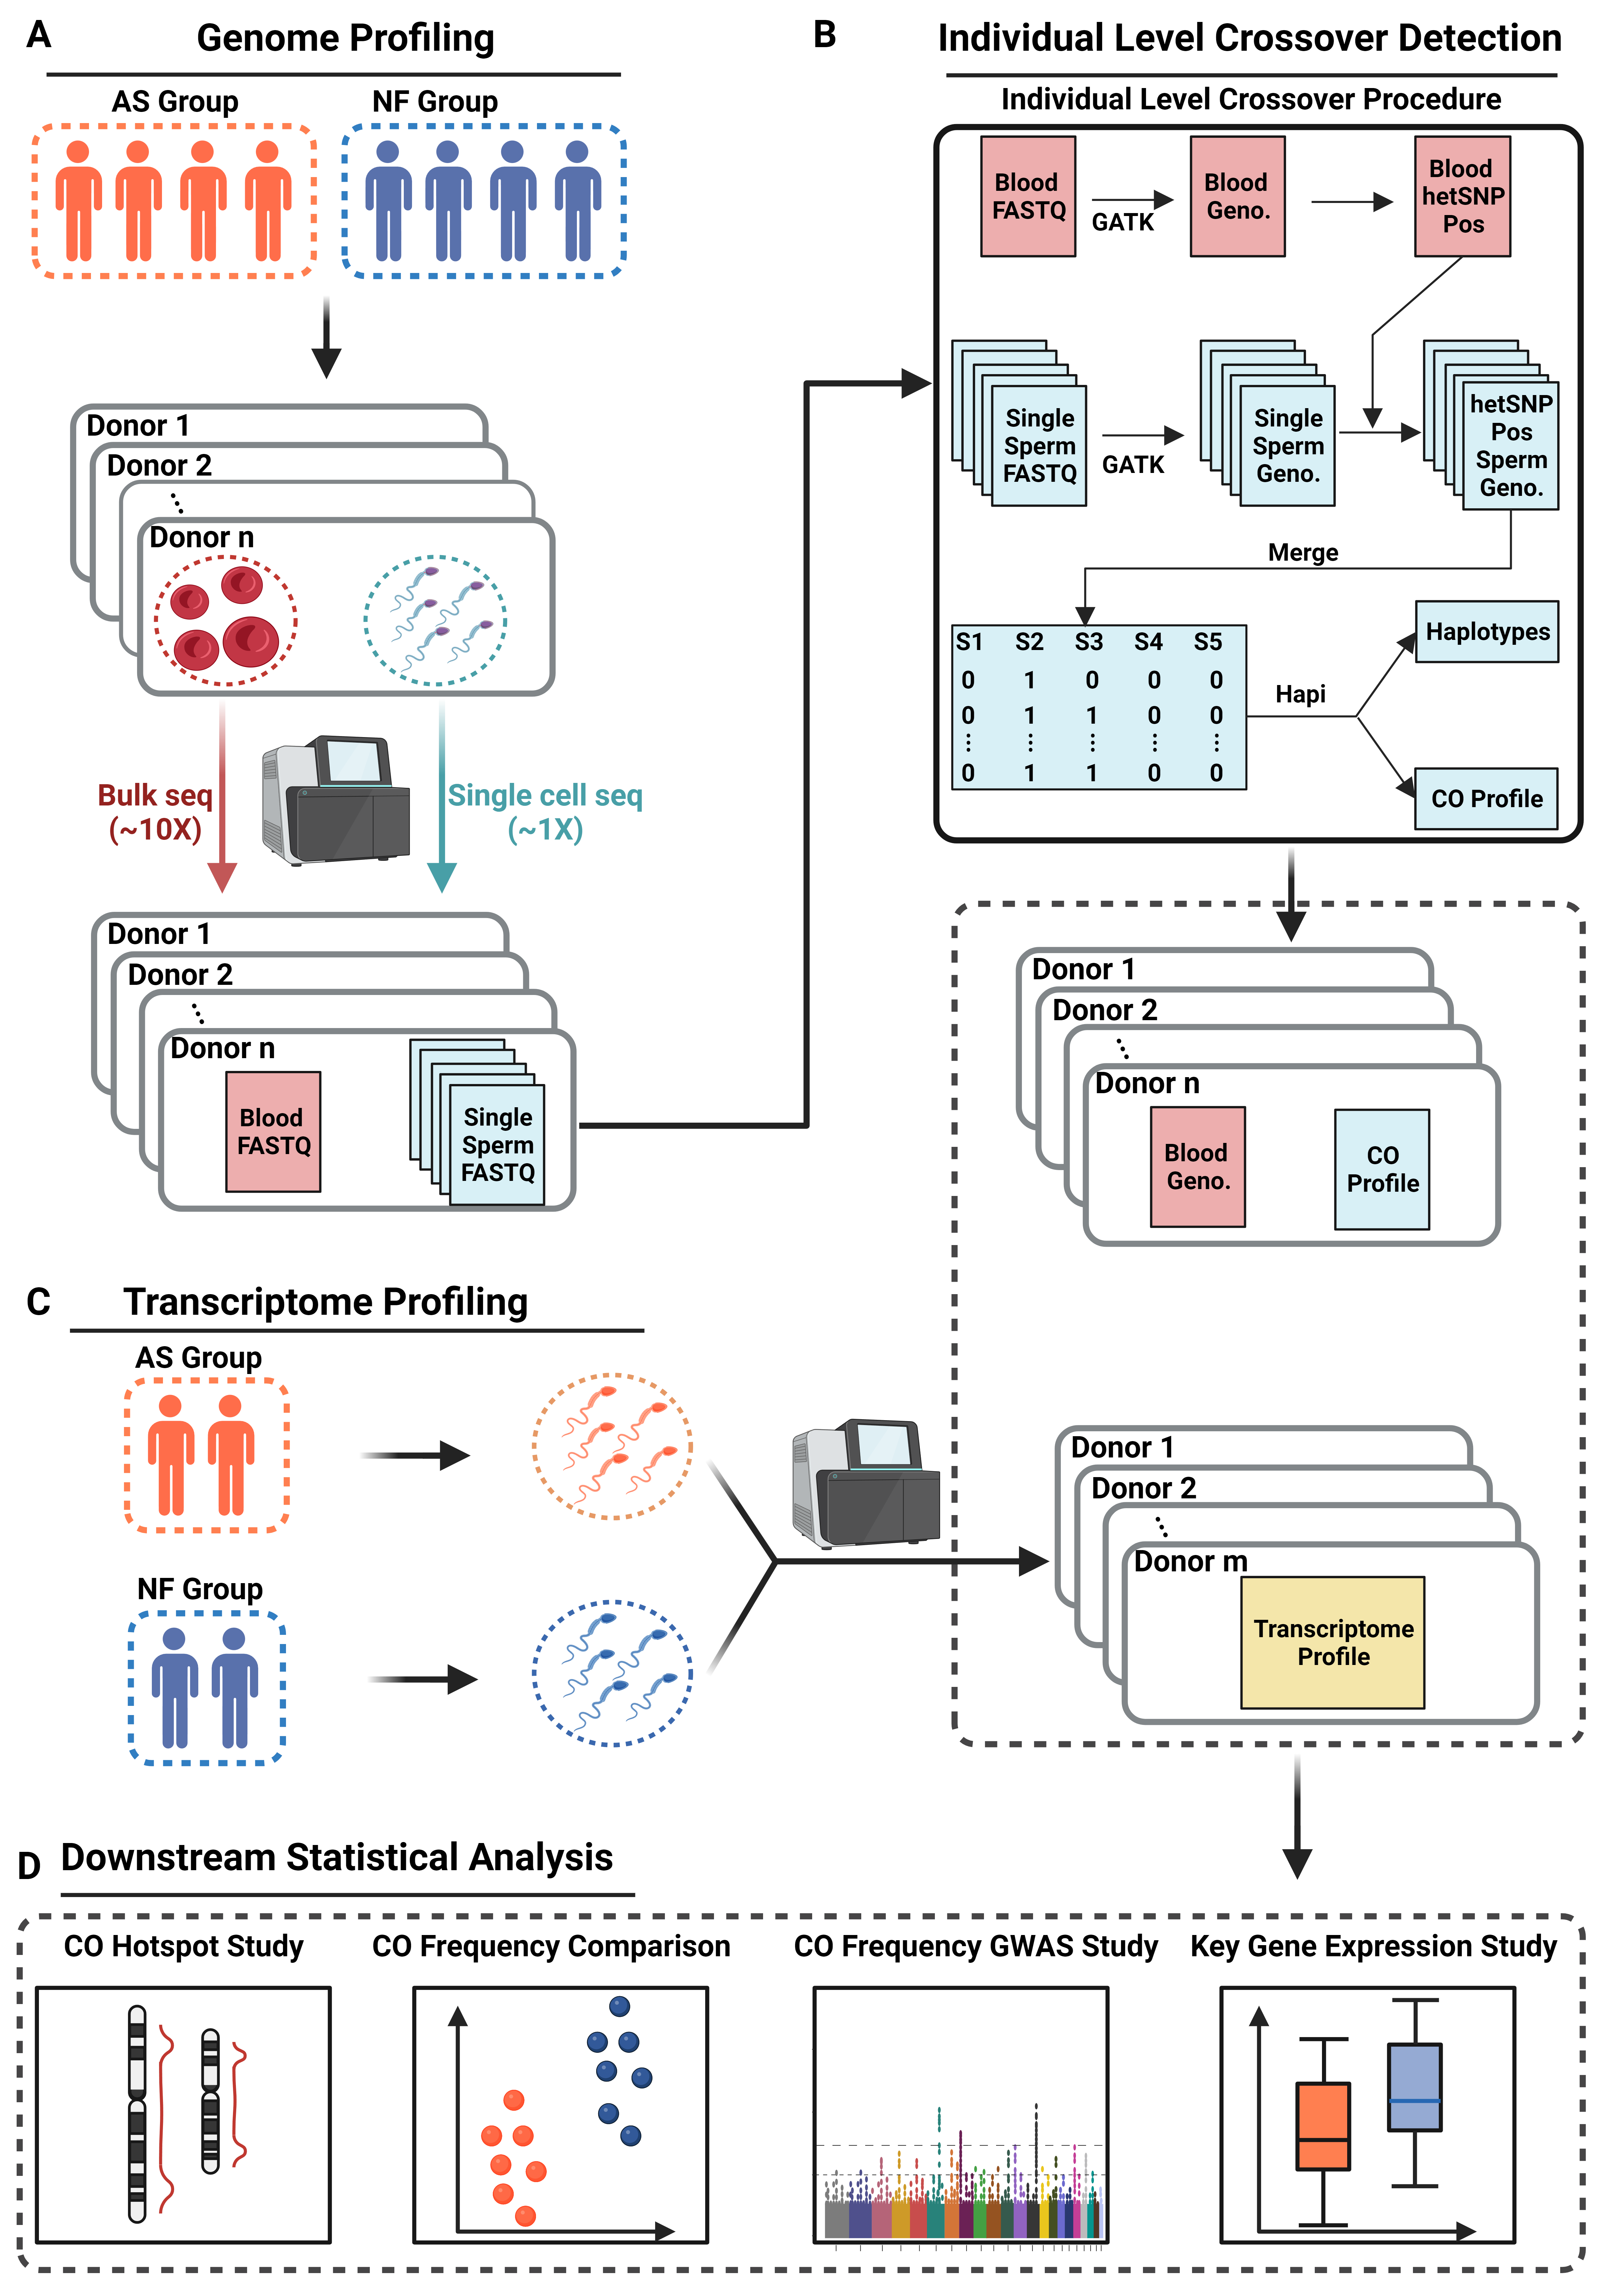
\includegraphics{Figures/s1.png}

}

\caption{Workflow for Comprehensive Analysis of Sperm Motility
Characteristics and Recombination. In this study, we outline the
comprehensive analysis workflow for assessing sperm motility
characteristics and recombination. (A) Genome Profile Phase. During the
genome profile phase, we collected blood samples and 4-5 sperm samples
from asthenospermia donors (n = 19) and normal donors (n = 11). Bulk
sequencing of blood samples was conducted at an approximate depth of
10x, while single-cell sequencing was performed on sperm cells at a
depth of 1x. For each donor, fastq files from bulk blood sequencing and
4-5 sperm single-cell fastq files were generated as part of the genome
profiling phase. (B) Individual-Level Crossover Detection Phase. During
the individual-level crossover detection phase, the Genome Analysis
Toolkit (GATK) genotyping pipeline was employed to obtain the genotypes
of both blood and sperm samples for each donor. Heterogeneous loci
positions were extracted from the blood genotype profile and
subsequently utilized as a reference for HAPI, enabling the
identification of crossover events in each sperm sample. By the
conclusion of this phase, both the blood genotype profile and the
crossover event profiles for each sperm sample were generated. (C)
Transcriptome Profiling Phase. In this phase, a second cohort consisting
of sperm samples from asthenospermia donors (n = 7) and normal donors (n
= 6) was collected. RNA-sequencing (RNA-seq) was performed to obtain the
gene expression profiles of these samples. (D) Downstream Statistics
Analysis Phase. In this phase, several key analyses were carried out,
including crossover hotspot analysis, a comparison of crossovers between
asthenospermia and normal sperm, an investigation into crossover
frequency-associated loci, and a comparison study of critical genes.}

\end{figure}

\bookmarksetup{startatroot}

\hypertarget{needed-packages}{%
\chapter{Needed Packages}\label{needed-packages}}

Load the needed packages. Below are the packages need in this documents.

\begin{Shaded}
\begin{Highlighting}[]
\FunctionTok{library}\NormalTok{(data.table)}
\FunctionTok{library}\NormalTok{(dplyr)}
\FunctionTok{library}\NormalTok{(stringr)}
\FunctionTok{library}\NormalTok{(ggplot2)}
\FunctionTok{library}\NormalTok{(karyoploteR)}
\FunctionTok{library}\NormalTok{(tibble)}
\FunctionTok{library}\NormalTok{(tidyr)}
\FunctionTok{library}\NormalTok{(Hapi)}
\FunctionTok{library}\NormalTok{(HMM)}
\FunctionTok{library}\NormalTok{(tidyverse)}
\FunctionTok{library}\NormalTok{(purrr)}
\FunctionTok{library}\NormalTok{(vcfR)}
\FunctionTok{library}\NormalTok{(DESeq2)}
\FunctionTok{library}\NormalTok{(ggplot2)}
\FunctionTok{library}\NormalTok{(ggrepel)}
\FunctionTok{library}\NormalTok{(biomaRt)}
\FunctionTok{library}\NormalTok{(stringr)}
\FunctionTok{library}\NormalTok{(tidyverse)}
\FunctionTok{library}\NormalTok{(reshape2)}
\FunctionTok{library}\NormalTok{(ggpubr)}
\FunctionTok{library}\NormalTok{(ggExtra)}
\FunctionTok{library}\NormalTok{(ggbeeswarm)}
\FunctionTok{library}\NormalTok{(GGally)}
\FunctionTok{library}\NormalTok{(regioneR)}
\FunctionTok{library}\NormalTok{(CopyNumberPlots)}
\FunctionTok{library}\NormalTok{(ggpmisc)}
\end{Highlighting}
\end{Shaded}

\bookmarksetup{startatroot}

\hypertarget{data-preparation}{%
\chapter{Data Preparation}\label{data-preparation}}

\hypertarget{gatk-genotyping}{%
\section{GATK Genotyping}\label{gatk-genotyping}}

Calling sperm genotype from fastq files were conducted by
\href{https://gatk.broadinstitute.org/hc/en-us}{GATK piplines}. This
code shows the work after getting the gvcf files. For the blood samples,
run whole GATK population SNP calling pipeline and get the vcf file.

\hypertarget{extract-the-key-features-of-vcf-files}{%
\section{Extract the key features of VCF
files}\label{extract-the-key-features-of-vcf-files}}

In order to check the correct filter for detecting the genotype, we
study the distribution of vcf features. The first step to do that is use
the bcftools to extract the key features of the VCF.

\begin{codelisting}

\caption{\texttt{Bash}}

\begin{Shaded}
\begin{Highlighting}[]
\CommentTok{\#!/bin/bash {-}l}

\DocumentationTok{\#\#\# A robust Bash header}
\CommentTok{\#This option prevents this, by terminating the script if any command exited with a nonzero exit status.}
\NormalTok{set }\SpecialCharTok{{-}}\NormalTok{e}
\NormalTok{set }\SpecialCharTok{{-}}\NormalTok{u}
\NormalTok{set }\SpecialCharTok{{-}}\NormalTok{o pipefail}
\DocumentationTok{\#\#\#}

\NormalTok{sperm\_sample\_nameList}\OtherTok{=}\StringTok{"../datasets/sperm\_sample\_namelist/sperm\_sample\_nameList.tsv"}

\ControlFlowTok{for}\NormalTok{ i }\ControlFlowTok{in}\NormalTok{ \{}\DecValTok{1}\NormalTok{..}\DecValTok{22}\NormalTok{\}}
\NormalTok{do}
\NormalTok{        echo }\StringTok{"Filtering chromosome$\{i\}"}

        \ControlFlowTok{while}\NormalTok{ read vcf\_file; do}
\NormalTok{                vcf\_input}\OtherTok{=}\StringTok{"../datasets/sperm\_vcf\_file/raw\_vcf/chr$\{i\}/$\{vcf\_file\}.vcf.gz"}
\NormalTok{                vcf\_features\_output}\OtherTok{=}\StringTok{"../datasets/sperm\_vcf\_file/extract\_feature\_raw\_vcf/chr$\{i\}/$\{vcf\_file\}.tsv"}
\NormalTok{                bcftools query }\SpecialCharTok{{-}}\NormalTok{f }\StringTok{\textquotesingle{}\%CHROM \%POS \%REF \%ALT [\%DP \%QUAL \%QD \%FS \%SOR \%MQRankSum \%ReadPosRankSum]}\SpecialCharTok{\textbackslash{}n}\StringTok{\textquotesingle{}} \SpecialCharTok{$}\NormalTok{\{vcf\_input\} }\SpecialCharTok{\textgreater{}} \ErrorTok{$}\NormalTok{\{vcf\_features\_output\}}

\NormalTok{        done }\SpecialCharTok{\textless{}}\ErrorTok{$}\NormalTok{\{sperm\_sample\_nameList\}}

\NormalTok{done}
\end{Highlighting}
\end{Shaded}

\end{codelisting}

\hypertarget{read-the-sperm-list}{%
\section{Read the sperm list}\label{read-the-sperm-list}}

We extract the sperm sample id and make the table that notes the sperm
id and donor id information.

\begin{codelisting}

\caption{\texttt{R script}}

\begin{Shaded}
\begin{Highlighting}[]
\NormalTok{sperm\_name\_list }\OtherTok{\textless{}{-}}\NormalTok{ data.table}\SpecialCharTok{::}\FunctionTok{fread}\NormalTok{(}\StringTok{"../datasets/sperm\_sample\_namelist/sperm\_sample\_nameList.tsv"}\NormalTok{,}
                         \AttributeTok{header=}\ConstantTok{FALSE}\NormalTok{) }\SpecialCharTok{\%\textgreater{}\%} \FunctionTok{as.data.frame}\NormalTok{()}

\FunctionTok{colnames}\NormalTok{(sperm\_name\_list) }\OtherTok{\textless{}{-}} \StringTok{"sperm\_ID"}

\NormalTok{sperm\_name\_list }\OtherTok{\textless{}{-}}\NormalTok{ sperm\_name\_list }\SpecialCharTok{\%\textgreater{}\%}\NormalTok{ dplyr}\SpecialCharTok{::}\FunctionTok{mutate}\NormalTok{(}\AttributeTok{donor\_ID =} \FunctionTok{gsub}\NormalTok{(}\StringTok{"s}\SpecialCharTok{\textbackslash{}\textbackslash{}}\StringTok{d+"}\NormalTok{, }\StringTok{""}\NormalTok{, sperm\_ID)) }\SpecialCharTok{\%\textgreater{}\%}
\NormalTok{                    dplyr}\SpecialCharTok{::}\FunctionTok{mutate}\NormalTok{(}\AttributeTok{donor\_ID =} \FunctionTok{gsub}\NormalTok{(}\StringTok{"N"}\NormalTok{, }\StringTok{"NF"}\NormalTok{, donor\_ID)) }\SpecialCharTok{\%\textgreater{}\%}
\NormalTok{                    dplyr}\SpecialCharTok{::}\FunctionTok{mutate}\NormalTok{(}\AttributeTok{donor\_ID =} \FunctionTok{gsub}\NormalTok{(}\StringTok{"NFF"}\NormalTok{, }\StringTok{"NF"}\NormalTok{, donor\_ID))}

\FunctionTok{fwrite}\NormalTok{(sperm\_name\_list, }\StringTok{"../datasets/sperm\_sample\_namelist/sperm\_name\_and\_donor\_nameList.csv"}\NormalTok{)}


\NormalTok{donor\_name\_list }\OtherTok{\textless{}{-}} \FunctionTok{unique}\NormalTok{(sperm\_name\_list}\SpecialCharTok{$}\NormalTok{donor\_ID)}
\end{Highlighting}
\end{Shaded}

\end{codelisting}

\hypertarget{check-the-coverage-of-the-vcf-files}{%
\section{Check the coverage of the VCF
files}\label{check-the-coverage-of-the-vcf-files}}

\begin{codelisting}

\caption{\texttt{R script}}

\begin{Shaded}
\begin{Highlighting}[]
\DocumentationTok{\#\# For each sperm, collect the chromosome features from 1 to 22}

\NormalTok{collect\_all\_chr }\OtherTok{\textless{}{-}} \ControlFlowTok{function}\NormalTok{(sperm\_name)\{}
  
\NormalTok{  sperm\_directory }\OtherTok{\textless{}{-}} \FunctionTok{paste0}\NormalTok{(}\StringTok{"../datasets/sperm\_vcf\_file/"}\NormalTok{, }\FunctionTok{c}\NormalTok{(}\DecValTok{1}\SpecialCharTok{:}\DecValTok{22}\NormalTok{), }\StringTok{"/"}\NormalTok{, sperm\_name, }\StringTok{".tsv"}\NormalTok{)}
  
\NormalTok{  all\_chromosomes }\OtherTok{\textless{}{-}} \FunctionTok{lapply}\NormalTok{(sperm\_directory, }\ControlFlowTok{function}\NormalTok{(i)\{}
  \FunctionTok{fread}\NormalTok{(i, }\AttributeTok{header=}\ConstantTok{FALSE}\NormalTok{)}
\NormalTok{  \})}
  
\NormalTok{  all\_chromosomes\_df }\OtherTok{\textless{}{-}} \FunctionTok{do.call}\NormalTok{(rbind.data.frame, all\_chromosomes)}
  
  \FunctionTok{colnames}\NormalTok{(all\_chromosomes\_df) }\OtherTok{\textless{}{-}} \FunctionTok{c}\NormalTok{(}\StringTok{"Chr"}\NormalTok{, }\StringTok{"Start"}\NormalTok{, }\StringTok{"DP"}\NormalTok{, }\StringTok{"QUAL"}\NormalTok{)}
  
\NormalTok{  all\_chromosomes\_df }\OtherTok{\textless{}{-}}\NormalTok{ all\_chromosomes\_df }\SpecialCharTok{\%\textgreater{}\%}\NormalTok{ dplyr}\SpecialCharTok{::}\FunctionTok{mutate}\NormalTok{(}\AttributeTok{End =}\NormalTok{ Start) }\SpecialCharTok{\%\textgreater{}\%} 
                        \FunctionTok{mutate\_at}\NormalTok{(}\FunctionTok{c}\NormalTok{(}\StringTok{"Start"}\NormalTok{, }\StringTok{"End"}\NormalTok{, }\StringTok{"DP"}\NormalTok{, }\StringTok{"QUAL"}\NormalTok{), as.numeric)}
  
  
\NormalTok{  all\_chromosomes\_df }\OtherTok{\textless{}{-}}\NormalTok{ all\_chromosomes\_df[, }\FunctionTok{c}\NormalTok{(}\StringTok{"Chr"}\NormalTok{, }\StringTok{"Start"}\NormalTok{, }\StringTok{"End"}\NormalTok{, }\StringTok{"DP"}\NormalTok{, }\StringTok{"QUAL"}\NormalTok{)]}
  
  
\NormalTok{  all\_chromosomes\_df }\OtherTok{\textless{}{-}}\NormalTok{ all\_chromosomes\_df }\SpecialCharTok{\%\textgreater{}\%}\NormalTok{ dplyr}\SpecialCharTok{::}\FunctionTok{filter}\NormalTok{(DP }\SpecialCharTok{!=} \DecValTok{0}\NormalTok{)}
  
\NormalTok{  all\_chromosomes\_DF\_GR }\OtherTok{\textless{}{-}} \FunctionTok{toGRanges}\NormalTok{(all\_chromosomes\_df)}
  
  \FunctionTok{return}\NormalTok{(all\_chromosomes\_DF\_GR)}
\NormalTok{\}}

\NormalTok{collect\_all\_sperm }\OtherTok{\textless{}{-}} \ControlFlowTok{function}\NormalTok{(donor\_name, sperm\_name\_list)\{}
  
\NormalTok{  sub\_sperm\_name\_list }\OtherTok{\textless{}{-}}\NormalTok{ sperm\_name\_list }\SpecialCharTok{\%\textgreater{}\%}\NormalTok{ dplyr}\SpecialCharTok{::}\FunctionTok{filter}\NormalTok{(donor\_ID }\SpecialCharTok{==}\NormalTok{ donor\_name)}
  
\NormalTok{  sperm\_feature\_list }\OtherTok{\textless{}{-}} \FunctionTok{lapply}\NormalTok{(sub\_sperm\_name\_list}\SpecialCharTok{$}\NormalTok{sperm\_ID, collect\_all\_chr)}
  
  \FunctionTok{names}\NormalTok{(sperm\_feature\_list) }\OtherTok{\textless{}{-}}\NormalTok{ sub\_sperm\_name\_list}\SpecialCharTok{$}\NormalTok{sperm\_ID}
    
  \FunctionTok{return}\NormalTok{(sperm\_feature\_list)}
                               
\NormalTok{\}}

\DocumentationTok{\#\# make\_SNP\_density\_plot }
\NormalTok{color\_panel }\OtherTok{\textless{}{-}} \FunctionTok{c}\NormalTok{(}\StringTok{"\#ddaacc"}\NormalTok{, }\StringTok{"\#0094ff"}\NormalTok{, }\StringTok{"\#ff9200"}\NormalTok{, }\StringTok{"\#008d00"}\NormalTok{, }\StringTok{"\#fb6f66"}\NormalTok{)}

\ControlFlowTok{for}\NormalTok{ (i }\ControlFlowTok{in}\NormalTok{ donor\_name\_list) \{}
    
\NormalTok{    sperm\_feature\_list }\OtherTok{\textless{}{-}} \FunctionTok{collect\_all\_sperm}\NormalTok{(i, sperm\_name\_list)}
    
\NormalTok{    pp }\OtherTok{\textless{}{-}} \FunctionTok{getDefaultPlotParams}\NormalTok{(}\AttributeTok{plot.type =} \DecValTok{4}\NormalTok{)}
\NormalTok{    pp}\SpecialCharTok{$}\NormalTok{data1inmargin }\OtherTok{\textless{}{-}} \DecValTok{0}
\NormalTok{    pp}\SpecialCharTok{$}\NormalTok{bottommargin }\OtherTok{\textless{}{-}} \DecValTok{20}
    
    \FunctionTok{pdf}\NormalTok{(}\FunctionTok{paste0}\NormalTok{(}\StringTok{"../figures/figure\_coverage\_density\_plot/"}\NormalTok{,}
\NormalTok{               i, }\StringTok{".pdf"}\NormalTok{), }
        \AttributeTok{width=}\DecValTok{22}\NormalTok{, }
        \AttributeTok{height=}\DecValTok{5}\NormalTok{)}
    
\NormalTok{    kp }\OtherTok{\textless{}{-}}\NormalTok{ karyoploteR}\SpecialCharTok{::}\FunctionTok{plotKaryotype}\NormalTok{(}\AttributeTok{genome=}\StringTok{"hg38"}\NormalTok{, }\AttributeTok{plot.type=}\DecValTok{4}\NormalTok{, }\AttributeTok{ideogram.plotter =} \ConstantTok{NULL}\NormalTok{,}
                    \AttributeTok{labels.plotter =} \ConstantTok{NULL}\NormalTok{, }\AttributeTok{plot.params =}\NormalTok{ pp,}
                    \AttributeTok{main=} \FunctionTok{paste0}\NormalTok{(}\StringTok{"SNP Density Plot of Donor:"}\NormalTok{, i), }
                    \AttributeTok{chromosomes =} \FunctionTok{paste0}\NormalTok{(}\StringTok{"chr"}\NormalTok{, }\FunctionTok{c}\NormalTok{(}\DecValTok{1}\SpecialCharTok{:}\DecValTok{22}\NormalTok{)))}
    
\NormalTok{    karyoploteR}\SpecialCharTok{::}\FunctionTok{kpAddCytobandsAsLine}\NormalTok{(kp)}
\NormalTok{    karyoploteR}\SpecialCharTok{::}\FunctionTok{kpAddChromosomeNames}\NormalTok{(kp, }\AttributeTok{srt=}\DecValTok{45}\NormalTok{)}
    
\NormalTok{    region\_vector }\OtherTok{\textless{}{-}} \FunctionTok{seq}\NormalTok{(}\DecValTok{0}\NormalTok{,}\DecValTok{1}\NormalTok{,}\AttributeTok{length.out =} \FunctionTok{length}\NormalTok{(sperm\_feature\_list) }\SpecialCharTok{+} \DecValTok{1}\NormalTok{)}
      
    \ControlFlowTok{for}\NormalTok{ (j }\ControlFlowTok{in} \FunctionTok{c}\NormalTok{(}\DecValTok{1}\SpecialCharTok{:}\FunctionTok{length}\NormalTok{(sperm\_feature\_list))) \{}
\NormalTok{      karyoploteR}\SpecialCharTok{::}\FunctionTok{kpPlotDensity}\NormalTok{(kp, sperm\_feature\_list[[j]], }\AttributeTok{window.size =} \FloatTok{10e4}\NormalTok{, }\AttributeTok{col=}\NormalTok{color\_panel[j], }\AttributeTok{r0=}\NormalTok{region\_vector[j],}
                    \AttributeTok{r1=}\NormalTok{region\_vector[j }\SpecialCharTok{+} \DecValTok{1}\NormalTok{])}
\NormalTok{      karyoploteR}\SpecialCharTok{::}\FunctionTok{kpAddLabels}\NormalTok{(kp, }\AttributeTok{labels=}\FunctionTok{names}\NormalTok{(sperm\_feature\_list)[j], }\AttributeTok{data.panel =} \DecValTok{1}\NormalTok{, }\AttributeTok{r0=}\NormalTok{region\_vector[j],}
                  \AttributeTok{r1=}\NormalTok{region\_vector[j }\SpecialCharTok{+} \DecValTok{1}\NormalTok{])}
\NormalTok{    \}}
    \FunctionTok{dev.off}\NormalTok{()}
\NormalTok{  \}}
\end{Highlighting}
\end{Shaded}

\end{codelisting}

\hypertarget{check-the-distribution-of-vcf-features}{%
\section{Check the Distribution of VCF
Features}\label{check-the-distribution-of-vcf-features}}

In the gvcf files, we have the key features

\begin{codelisting}

\caption{\texttt{R script}}

\begin{Shaded}
\begin{Highlighting}[]
\NormalTok{collect\_all\_chr\_features }\OtherTok{\textless{}{-}} \ControlFlowTok{function}\NormalTok{(sperm\_name)\{}
  
\NormalTok{  sperm\_directory }\OtherTok{\textless{}{-}} \FunctionTok{paste0}\NormalTok{(}\StringTok{"../datasets/sperm\_vcf\_file/extract\_feature/chr"}\NormalTok{, }\FunctionTok{c}\NormalTok{(}\DecValTok{1}\SpecialCharTok{:}\DecValTok{22}\NormalTok{), }\StringTok{"/"}\NormalTok{, sperm\_name, }\StringTok{".tsv"}\NormalTok{)}
  
\NormalTok{  all\_chromosomes }\OtherTok{\textless{}{-}} \FunctionTok{lapply}\NormalTok{(sperm\_directory, }\ControlFlowTok{function}\NormalTok{(i)\{}
  \FunctionTok{fread}\NormalTok{(i, }\AttributeTok{header=}\ConstantTok{FALSE}\NormalTok{)}
\NormalTok{  \})}
  
\NormalTok{  all\_chromosomes\_df }\OtherTok{\textless{}{-}} \FunctionTok{do.call}\NormalTok{(rbind.data.frame, all\_chromosomes)}
  
  \FunctionTok{colnames}\NormalTok{(all\_chromosomes\_df) }\OtherTok{\textless{}{-}} \FunctionTok{c}\NormalTok{(}\StringTok{"Chr"}\NormalTok{, }\StringTok{"Start"}\NormalTok{, }\StringTok{"DP"}\NormalTok{, }\StringTok{"QUAL"}\NormalTok{, }\StringTok{"QD"}\NormalTok{, }\StringTok{"FS"}\NormalTok{, }\StringTok{"SOR"}\NormalTok{, }\StringTok{"MQRankSum"}\NormalTok{, }\StringTok{"ReadPosRankSum"}\NormalTok{)}
  
\NormalTok{  all\_chromosomes\_df }\OtherTok{\textless{}{-}}\NormalTok{ all\_chromosomes\_df }\SpecialCharTok{\%\textgreater{}\%}\NormalTok{ dplyr}\SpecialCharTok{::}\FunctionTok{mutate}\NormalTok{(}\AttributeTok{End =}\NormalTok{ Start) }\SpecialCharTok{\%\textgreater{}\%} 
                        \FunctionTok{mutate\_at}\NormalTok{(}\FunctionTok{c}\NormalTok{(}\StringTok{"Start"}\NormalTok{, }\StringTok{"End"}\NormalTok{, }\StringTok{"DP"}\NormalTok{, }\StringTok{"QUAL"}\NormalTok{, }\StringTok{"QD"}\NormalTok{, }\StringTok{"FS"}\NormalTok{, }\StringTok{"SOR"}\NormalTok{, }\StringTok{"MQRankSum"}\NormalTok{, }\StringTok{"ReadPosRankSum"}\NormalTok{), as.numeric)}
  
  
\NormalTok{  all\_chromosomes\_df }\OtherTok{\textless{}{-}}\NormalTok{ all\_chromosomes\_df[, }\FunctionTok{c}\NormalTok{(}\StringTok{"Chr"}\NormalTok{, }\StringTok{"Start"}\NormalTok{, }\StringTok{"End"}\NormalTok{, }\StringTok{"DP"}\NormalTok{, }\StringTok{"QUAL"}\NormalTok{, }\StringTok{"QD"}\NormalTok{, }\StringTok{"FS"}\NormalTok{, }\StringTok{"SOR"}\NormalTok{, }\StringTok{"MQRankSum"}\NormalTok{, }\StringTok{"ReadPosRankSum"}\NormalTok{)]}
  
  
\NormalTok{  all\_chromosomes\_df }\OtherTok{\textless{}{-}}\NormalTok{ all\_chromosomes\_df }\SpecialCharTok{\%\textgreater{}\%}\NormalTok{ dplyr}\SpecialCharTok{::}\FunctionTok{filter}\NormalTok{(DP }\SpecialCharTok{!=} \DecValTok{0}\NormalTok{)}
  
  \FunctionTok{return}\NormalTok{(all\_chromosomes\_df)}
\NormalTok{\}}


\NormalTok{collect\_all\_sperm\_features }\OtherTok{\textless{}{-}} \ControlFlowTok{function}\NormalTok{(donor\_name, sperm\_name\_list)\{}
  
\NormalTok{  sub\_sperm\_name\_list }\OtherTok{\textless{}{-}}\NormalTok{ sperm\_name\_list }\SpecialCharTok{\%\textgreater{}\%}\NormalTok{ dplyr}\SpecialCharTok{::}\FunctionTok{filter}\NormalTok{(donor\_ID }\SpecialCharTok{==}\NormalTok{ donor\_name)}
  
\NormalTok{  sperm\_feature\_list }\OtherTok{\textless{}{-}} \FunctionTok{lapply}\NormalTok{(sub\_sperm\_name\_list}\SpecialCharTok{$}\NormalTok{sperm\_ID, collect\_all\_chr\_features)}
  
  \FunctionTok{names}\NormalTok{(sperm\_feature\_list) }\OtherTok{\textless{}{-}}\NormalTok{ sub\_sperm\_name\_list}\SpecialCharTok{$}\NormalTok{sperm\_ID}
    
  \FunctionTok{return}\NormalTok{(sperm\_feature\_list)}
                               
\NormalTok{\}}


\ControlFlowTok{for}\NormalTok{ (i }\ControlFlowTok{in}\NormalTok{ donor\_name\_list) \{}
  
\NormalTok{  donor }\OtherTok{\textless{}{-}} \FunctionTok{collect\_all\_sperm\_features}\NormalTok{(i, sperm\_name\_list)}
  
\NormalTok{  donor }\OtherTok{\textless{}{-}}\NormalTok{ dplyr}\SpecialCharTok{::}\FunctionTok{bind\_rows}\NormalTok{(donor, }\AttributeTok{.id =} \StringTok{"sperm\_ID"}\NormalTok{)}
  
\NormalTok{  donor }\OtherTok{\textless{}{-}}\NormalTok{ donor }\SpecialCharTok{\%\textgreater{}\%}\NormalTok{ dplyr}\SpecialCharTok{::}\FunctionTok{select}\NormalTok{(}\SpecialCharTok{{-}}\FunctionTok{c}\NormalTok{(Chr, Start, End))}
  
\NormalTok{  donor }\OtherTok{\textless{}{-}} \FunctionTok{melt}\NormalTok{(donor, }\AttributeTok{id=}\FunctionTok{c}\NormalTok{(}\StringTok{"sperm\_ID"}\NormalTok{))}
  
 
  
  \CommentTok{\# Density plot in ggplot2}
  
  \FunctionTok{ggplot}\NormalTok{(donor, }\FunctionTok{aes}\NormalTok{(}\AttributeTok{x =}\NormalTok{ value)) }\SpecialCharTok{+} \FunctionTok{geom\_density}\NormalTok{(}\AttributeTok{color =} \DecValTok{4}\NormalTok{, }\AttributeTok{fill =} \DecValTok{4}\NormalTok{, }\AttributeTok{alpha =} \FloatTok{0.25}\NormalTok{) }\SpecialCharTok{+} 
    \FunctionTok{theme\_bw}\NormalTok{() }\SpecialCharTok{+} 
    \FunctionTok{theme}\NormalTok{(}\AttributeTok{axis.text.x =} \FunctionTok{element\_text}\NormalTok{(}\AttributeTok{angle =} \DecValTok{45}\NormalTok{, }\AttributeTok{vjust =} \FloatTok{0.5}\NormalTok{)) }\SpecialCharTok{+} 
    \FunctionTok{facet\_grid}\NormalTok{(}\FunctionTok{vars}\NormalTok{(sperm\_ID), }\FunctionTok{vars}\NormalTok{(variable), }\AttributeTok{scales =} \StringTok{"free"}\NormalTok{)}
  
  \FunctionTok{ggsave}\NormalTok{(}\FunctionTok{paste0}\NormalTok{(}\StringTok{"../figures/figure\_coverage\_density\_plot/"}\NormalTok{,}
\NormalTok{               i, }\StringTok{".pdf"}\NormalTok{), }
        \AttributeTok{width=}\DecValTok{14}\NormalTok{, }
        \AttributeTok{height=}\DecValTok{10}\NormalTok{)}

\NormalTok{\}}
\end{Highlighting}
\end{Shaded}

\end{codelisting}

\hypertarget{filter-the-vcf-file}{%
\section{Filter the vcf file}\label{filter-the-vcf-file}}

Based on the raw gvcf file, we use the ``(QUAL\textgreater10)
\textbar\textbar{} (ALT=''.''\&FMT/RGQ\textgreater50)'' to filter the
genotypes. This procedure was conducted by bcftools.

\begin{codelisting}

\caption{\texttt{bash script}}

\begin{Shaded}
\begin{Highlighting}[]
\NormalTok{sperm\_sample\_nameList}\OtherTok{=}\StringTok{"../datasets/sperm\_sample\_namelist/sperm\_sample\_nameList.tsv"}

\NormalTok{        echo }\StringTok{"Extract VCF: QUAL\_and\_no\_ALT"}

        \ControlFlowTok{for}\NormalTok{ i }\ControlFlowTok{in}\NormalTok{ chr\{}\DecValTok{1}\NormalTok{..}\DecValTok{22}\NormalTok{\}}
\NormalTok{        do}
\NormalTok{                echo }\StringTok{"chr: $\{i\}"}

                \ControlFlowTok{while}\NormalTok{ read vcf\_file; do}

\NormalTok{                        vcf\_input}\OtherTok{=}\StringTok{"../datasets/sperm\_vcf\_file/raw\_vcf/chr$\{i\}/$\{vcf\_file\}.vcf.gz"}
\NormalTok{                        vcf\_output}\OtherTok{=}\StringTok{"../datasets/sperm\_vcf\_file/selected\_vcf/QUAL\_and\_RGQ/chr$\{i\}/$\{vcf\_file\}.vcf.gz"}

                        \CommentTok{\#echo "vcf input directory: $\{vcf\_input\}"}
                        \CommentTok{\#echo "vcf output directory: $\{vcf\_output\}"}

\NormalTok{                        bcftools view }\SpecialCharTok{{-}}\NormalTok{O z }\SpecialCharTok{{-}}\NormalTok{o }\SpecialCharTok{$}\NormalTok{\{vcf\_output\} }\SpecialCharTok{{-}}\NormalTok{i }\StringTok{\textquotesingle{}(QUAL\textgreater{}10) || (ALT="."\&FMT/RGQ\textgreater{}50)\textquotesingle{}} \SpecialCharTok{$}\NormalTok{\{vcf\_input\}}

\NormalTok{                done }\SpecialCharTok{\textless{}}\ErrorTok{$}\NormalTok{\{sperm\_sample\_nameList\}}
\NormalTok{        done}
\end{Highlighting}
\end{Shaded}

\end{codelisting}

\bookmarksetup{startatroot}

\hypertarget{aneuploidy-test}{%
\chapter{Aneuploidy Test}\label{aneuploidy-test}}

\hypertarget{sequencing-depth-in-windows}{%
\section{Sequencing Depth in
windows}\label{sequencing-depth-in-windows}}

Based on the aligned sperm sequence and blood sequence, we can use
\href{https://github.com/hliang/cnv-seq}{cnvseq} to call the depth in
slide window and the CNV.

\begin{codelisting}

\caption{\texttt{R script (Need to delete)}}

\begin{Shaded}
\begin{Highlighting}[]
\NormalTok{cnv\_count\_directory }\OtherTok{\textless{}{-}} \StringTok{"../datasets/sperm\_cnv\_windows/"}
\NormalTok{figure\_out\_directory }\OtherTok{\textless{}{-}} \StringTok{"../figures/figure\_cnv\_plot/"}

\NormalTok{fileList }\OtherTok{\textless{}{-}} \FunctionTok{list.files}\NormalTok{(}\AttributeTok{path =}\NormalTok{ cnv\_count\_directory, }\AttributeTok{pattern =} \StringTok{"*.cnv$"}\NormalTok{, }\AttributeTok{all.files =} \ConstantTok{FALSE}\NormalTok{,}
                       \AttributeTok{full.names =} \ConstantTok{FALSE}\NormalTok{, }\AttributeTok{recursive =} \ConstantTok{FALSE}\NormalTok{, }\AttributeTok{ignore.case =} \ConstantTok{FALSE}\NormalTok{, }\AttributeTok{include.dirs =} \ConstantTok{FALSE}\NormalTok{, }\AttributeTok{no.. =} \ConstantTok{FALSE}\NormalTok{)}

\NormalTok{CNV\_list }\OtherTok{\textless{}{-}} \FunctionTok{list}\NormalTok{()}

\ControlFlowTok{for}\NormalTok{ (sperm\_count\_file }\ControlFlowTok{in}\NormalTok{ fileList) \{}
  
\NormalTok{  sperm\_ID }\OtherTok{\textless{}{-}} \FunctionTok{gsub}\NormalTok{(}\StringTok{"}\SpecialCharTok{\textbackslash{}\textbackslash{}}\StringTok{..*"}\NormalTok{,}\StringTok{""}\NormalTok{, sperm\_count\_file)}
  
  \DocumentationTok{\#\# Input the output from cnv{-}seq}
\NormalTok{  cnv }\OtherTok{\textless{}{-}} \FunctionTok{read.table}\NormalTok{(}\FunctionTok{paste0}\NormalTok{(cnv\_count\_directory, sperm\_count\_file), }\AttributeTok{header =}\NormalTok{ T)}
  
  \DocumentationTok{\#\# Extract the cnv in chr1 to chr22 and chrX and chrY}
\NormalTok{  cnv }\OtherTok{\textless{}{-}}\NormalTok{ cnv[cnv}\SpecialCharTok{$}\NormalTok{chromosome }\SpecialCharTok{\%in\%} \FunctionTok{c}\NormalTok{(}\FunctionTok{paste0}\NormalTok{(}\StringTok{"chr"}\NormalTok{, }\FunctionTok{c}\NormalTok{(}\DecValTok{1}\SpecialCharTok{:}\DecValTok{22}\NormalTok{))), ]}
  
\NormalTok{  cnv}\SpecialCharTok{$}\NormalTok{chromosome }\OtherTok{\textless{}{-}} \FunctionTok{factor}\NormalTok{(cnv}\SpecialCharTok{$}\NormalTok{chromosome, }\AttributeTok{levels =} \FunctionTok{c}\NormalTok{(}\FunctionTok{paste0}\NormalTok{(}\StringTok{"chr"}\NormalTok{, }\FunctionTok{c}\NormalTok{(}\DecValTok{1}\SpecialCharTok{:}\DecValTok{22}\NormalTok{))))}
  
\NormalTok{  cnv }\OtherTok{\textless{}{-}}\NormalTok{ cnv[}\FunctionTok{order}\NormalTok{(cnv}\SpecialCharTok{$}\NormalTok{chromosome),]}
  
  \DocumentationTok{\#\# cnv$color \textless{}{-} colByChr(as.character(cnv$chromosome), colors = "2blues")}
  
  \FunctionTok{rownames}\NormalTok{(cnv) }\OtherTok{\textless{}{-}} \ConstantTok{NULL}
  
  \DocumentationTok{\#\# Delete the log2 NA}
\NormalTok{  cnv }\OtherTok{\textless{}{-}}\NormalTok{ cnv[}\SpecialCharTok{!}\FunctionTok{is.na}\NormalTok{(cnv}\SpecialCharTok{$}\NormalTok{log2), ]}
  
  \DocumentationTok{\#\#\# Assign (pos or neg) sign to the cnv value}
\NormalTok{  cnv}\SpecialCharTok{$}\NormalTok{cn.withDir }\OtherTok{\textless{}{-}} \FunctionTok{ifelse}\NormalTok{(}\FunctionTok{is.na}\NormalTok{(cnv}\SpecialCharTok{$}\NormalTok{cnv.log2), }\DecValTok{0}\NormalTok{, cnv}\SpecialCharTok{$}\NormalTok{cnv.log2)}
  
\NormalTok{  CNV\_list[[sperm\_ID]] }\OtherTok{\textless{}{-}}\NormalTok{ cnv}
    
\NormalTok{  cnv\_GRanges }\OtherTok{\textless{}{-}} \FunctionTok{makeGRangesFromDataFrame}\NormalTok{(cnv)}
  
  
\NormalTok{  cnv\_GRanges}\SpecialCharTok{$}\NormalTok{lrr }\OtherTok{\textless{}{-}}\NormalTok{ cnv}\SpecialCharTok{$}\NormalTok{log2}
  
  
  \CommentTok{\# cnv\_GRanges$cn \textless{}{-} cnv$cnv.log2}
  \CommentTok{\# cnv\_GRanges$color \textless{}{-} cnv$color}
    
\NormalTok{  cncalls }\OtherTok{\textless{}{-}} \FunctionTok{loadCopyNumberCalls}\NormalTok{(cnv, }\AttributeTok{cn.col=}\StringTok{"cn.withDir"}\NormalTok{)}
  
  \DocumentationTok{\#\# }
  \ControlFlowTok{if}\NormalTok{(}\ConstantTok{FALSE}\NormalTok{)\{}
    
    \FunctionTok{pdf}\NormalTok{(}\FunctionTok{paste0}\NormalTok{(figure\_out\_directory, sperm\_ID, }\StringTok{".pdf"}\NormalTok{), }\AttributeTok{width =} \FloatTok{8.3}\NormalTok{, }\AttributeTok{height =} \DecValTok{2}\NormalTok{)}
    
\NormalTok{    kp }\OtherTok{\textless{}{-}} \FunctionTok{plotKaryotype}\NormalTok{(}\StringTok{"hg38"}\NormalTok{, }\AttributeTok{plot.type =} \DecValTok{4}\NormalTok{, }\AttributeTok{labels.plotter =} \ConstantTok{NULL}\NormalTok{, }\AttributeTok{main=}\StringTok{""}\NormalTok{, }\AttributeTok{cex=}\FloatTok{0.02}\NormalTok{,}
                        \AttributeTok{chromosomes=}\FunctionTok{paste0}\NormalTok{(}\StringTok{"chr"}\NormalTok{, }\FunctionTok{c}\NormalTok{(}\DecValTok{1}\SpecialCharTok{:}\DecValTok{22}\NormalTok{)),}
                        \AttributeTok{ideogram.plotter    =} \ConstantTok{NULL}\NormalTok{)}
    
    \CommentTok{\# Plot the ideogram as a line}
    \FunctionTok{kpAddCytobandsAsLine}\NormalTok{(kp)}
    
    \FunctionTok{kpAddChromosomeNames}\NormalTok{(kp, }\AttributeTok{srt=}\DecValTok{45}\NormalTok{, }\AttributeTok{cex=}\FloatTok{0.8}\NormalTok{)}
    
    \CommentTok{\#plotLRR(kp, cnv\_GRanges, ymin={-}5, ymax=5, labels = NA, out.of.range = "points", out.of.range.col="red",points.col = "\#AAAAAAAA", line.at.0 = FALSE, points.cex = 3, add.axis = FALSE)}
  
    \CommentTok{\# Modify the "lrr" values to be at most 5}
\NormalTok{    cnv\_GRanges}\SpecialCharTok{$}\NormalTok{lrr }\OtherTok{\textless{}{-}} \FunctionTok{pmin}\NormalTok{(}\FunctionTok{abs}\NormalTok{(cnv\_GRanges}\SpecialCharTok{$}\NormalTok{lrr), }\DecValTok{5}\NormalTok{) }\SpecialCharTok{*} \FunctionTok{sign}\NormalTok{(cnv\_GRanges}\SpecialCharTok{$}\NormalTok{lrr)}
  
    \FunctionTok{plotLRR}\NormalTok{(kp,}
\NormalTok{            cnv\_GRanges, }
            \AttributeTok{ymin=}\SpecialCharTok{{-}}\DecValTok{4}\NormalTok{, }
            \AttributeTok{ymax=}\DecValTok{4}\NormalTok{, }
            \AttributeTok{labels =} \ConstantTok{NA}\NormalTok{, }
            \AttributeTok{out.of.range =} \StringTok{"points"}\NormalTok{, }
            \AttributeTok{out.of.range.col=}\StringTok{"\#DC0000FF"}\NormalTok{, }
            \AttributeTok{points.col =} \StringTok{"\#AAAAAAAA"}\NormalTok{, }
            \AttributeTok{line.at.0 =} \ConstantTok{FALSE}\NormalTok{, }
            \AttributeTok{points.cex =} \FloatTok{0.8}\NormalTok{, }
            \AttributeTok{add.axis =} \ConstantTok{FALSE}\NormalTok{)}
  
  
  \CommentTok{\#plotCopyNumberCallsAsLines(kp, cn.calls = cncalls, ymin={-}2, ymax=2, lwd=6, add.axis=FALSE, labels = NA, col="\#48B774", style="segments", r0=0.4, r1=0.6)}
  
  \FunctionTok{kpAddChromosomeSeparators}\NormalTok{(kp, }\AttributeTok{lwd=}\FloatTok{1.5}\NormalTok{, }\AttributeTok{col =} \StringTok{"\#666666"}\NormalTok{)}
  \FunctionTok{kpAxis}\NormalTok{(kp, }\AttributeTok{ymin =} \SpecialCharTok{{-}}\DecValTok{5}\NormalTok{, }\AttributeTok{ymax=}\DecValTok{5}\NormalTok{, }\AttributeTok{tick.pos =} \SpecialCharTok{{-}}\DecValTok{5}\SpecialCharTok{:}\DecValTok{5}\NormalTok{, }\AttributeTok{cex=}\FloatTok{0.8}\NormalTok{, }\AttributeTok{offset =} \FloatTok{0.1}\NormalTok{)}
  \FunctionTok{kpAddLabels}\NormalTok{(kp, }\AttributeTok{labels =} \StringTok{"Log2 Ratio"}\NormalTok{, }\AttributeTok{cex=}\FloatTok{0.8}\NormalTok{, }\AttributeTok{srt=}\DecValTok{90}\NormalTok{, }\AttributeTok{pos=}\DecValTok{3}\NormalTok{, }\AttributeTok{label.margin =} \FloatTok{0.03}\NormalTok{)}
  \CommentTok{\# Add a title to the karyoplot using the title function}
  \FunctionTok{kpAddMainTitle}\NormalTok{(kp, sperm\_ID, }\AttributeTok{cex=}\DecValTok{1}\NormalTok{)}
  \FunctionTok{kpAbline}\NormalTok{(kp, }\AttributeTok{h=}\FloatTok{0.5}\NormalTok{, }\AttributeTok{col=}\StringTok{"black"}\NormalTok{, }\AttributeTok{lwd=}\DecValTok{2}\NormalTok{)}

  
  \FunctionTok{dev.off}\NormalTok{()}
\NormalTok{  \}}
\NormalTok{\}}
\end{Highlighting}
\end{Shaded}

\end{codelisting}

\bookmarksetup{startatroot}

\hypertarget{prepare-the-input-data-for-hapi}{%
\chapter{Prepare the input data for
HAPI}\label{prepare-the-input-data-for-hapi}}

Followed by the last Chapter, we get the filtered SNP positions and next
we need to make the sperm VCF files into a R matrix for Hapi. Since
genotype phasing and crossover detect only needs heterzygous loci as
input, we use the blood sample to get this information then combine with
the corresponding positions in sperm to get the matrix.

\hypertarget{prepare-the-aneuploidy-removed-sperm-name-list}{%
\section{Prepare the aneuploidy removed sperm name
list}\label{prepare-the-aneuploidy-removed-sperm-name-list}}

\hypertarget{generate-the-hpai-input-matrix}{%
\section{Generate the Hpai input
matrix}\label{generate-the-hpai-input-matrix}}

\begin{codelisting}

\caption{\texttt{R script}}

\begin{Shaded}
\begin{Highlighting}[]
\NormalTok{chr\_id }\OtherTok{\textless{}{-}} \DecValTok{1}

\NormalTok{blood\_gt\_chr }\OtherTok{\textless{}{-}} \FunctionTok{readRDS}\NormalTok{(}\FunctionTok{paste0}\NormalTok{(}\StringTok{"../datasets/simplified\_blood\_gt\_by\_chr/simplified\_blood\_gt\_by\_chr"}\NormalTok{, chr\_id, }\StringTok{".rds"}\NormalTok{))}

\NormalTok{SPERM\_DIRECTORY }\OtherTok{\textless{}{-}} \FunctionTok{paste0}\NormalTok{(}\StringTok{"../datasets/sperm\_vcf\_file/selected\_vcf/QUAL\_and\_RGQ/chr"}\NormalTok{, chr\_id, }\StringTok{"/"}\NormalTok{)}


\NormalTok{sperm\_list }\OtherTok{\textless{}{-}} \FunctionTok{list.files}\NormalTok{(}\AttributeTok{path =}\NormalTok{ SPERM\_DIRECTORY, }\AttributeTok{pattern =} \StringTok{"*.vcf.gz$"}\NormalTok{, }\AttributeTok{all.files =} \ConstantTok{FALSE}\NormalTok{, }
                              \AttributeTok{full.names =} \ConstantTok{FALSE}\NormalTok{, }\AttributeTok{recursive =} \ConstantTok{FALSE}\NormalTok{,}
                              \AttributeTok{ignore.case =} \ConstantTok{FALSE}\NormalTok{, }\AttributeTok{include.dirs =} \ConstantTok{FALSE}\NormalTok{, }\AttributeTok{no.. =} \ConstantTok{FALSE}\NormalTok{)}

\NormalTok{sperm\_list\_df }\OtherTok{\textless{}{-}} \FunctionTok{gsub}\NormalTok{(}\StringTok{"}\SpecialCharTok{\textbackslash{}\textbackslash{}}\StringTok{.vcf}\SpecialCharTok{\textbackslash{}\textbackslash{}}\StringTok{.gz"}\NormalTok{, }\StringTok{""}\NormalTok{, sperm\_list)  }
\NormalTok{sperm\_list\_df }\OtherTok{\textless{}{-}} \FunctionTok{as.data.frame}\NormalTok{(sperm\_list\_df)}

\CommentTok{\#write.table(sperm\_list\_df, }
\CommentTok{\#            file = "D:/sperm\_project/sperm\_vcf\_file/sperm\_sampleList/sperm\_sample\_nameList.tsv", }
\CommentTok{\#            append = F, sep = "\textbackslash{}t", row.names=FALSE, col.names=FALSE, quote=FALSE)}



\DocumentationTok{\#\# Merge to the matrix}

\NormalTok{patient\_name }\OtherTok{\textless{}{-}} \FunctionTok{gsub}\NormalTok{(}\StringTok{"s}\SpecialCharTok{\textbackslash{}\textbackslash{}}\StringTok{d}\SpecialCharTok{\textbackslash{}\textbackslash{}}\StringTok{.vcf}\SpecialCharTok{\textbackslash{}\textbackslash{}}\StringTok{.gz"}\NormalTok{, }\StringTok{""}\NormalTok{, sperm\_list)}
\NormalTok{patient\_name }\OtherTok{\textless{}{-}} \FunctionTok{unique}\NormalTok{(patient\_name)}

\ControlFlowTok{for}\NormalTok{ (chr\_id }\ControlFlowTok{in} \FunctionTok{c}\NormalTok{(}\DecValTok{1}\SpecialCharTok{:}\DecValTok{22}\NormalTok{)) \{}
  \DocumentationTok{\#\# Print the current working chrosome}
  
  \FunctionTok{print}\NormalTok{(}\StringTok{"Chromosome:"}\NormalTok{)}
  \FunctionTok{print}\NormalTok{(chr\_id)}
  
  \DocumentationTok{\#\# Read the blood genotype by chromosome}
\NormalTok{  blood\_gt\_chr }\OtherTok{\textless{}{-}} \FunctionTok{readRDS}\NormalTok{(}\FunctionTok{paste0}\NormalTok{(}\StringTok{"../datasets/simplified\_blood\_gt\_by\_chr/simplified\_blood\_gt\_by\_chr"}\NormalTok{, chr\_id, }\StringTok{".rds"}\NormalTok{))}
  
  \DocumentationTok{\#\# The Directory of filter sperm vcf file}
\NormalTok{  Filtered\_SPERM\_DIRECTORY }\OtherTok{\textless{}{-}} \FunctionTok{paste0}\NormalTok{(}\StringTok{"../datasets/sperm\_vcf\_file/selected\_vcf/QUAL\_and\_RGQ/chr"}\NormalTok{, chr\_id, }\StringTok{"/"}\NormalTok{)}
  
  \DocumentationTok{\#\# Initate the Hapi Input Matirx List}
  
\NormalTok{  Hapi\_input\_matrix\_List }\OtherTok{\textless{}{-}} \FunctionTok{list}\NormalTok{()}
  
  \ControlFlowTok{for}\NormalTok{ (patient }\ControlFlowTok{in}\NormalTok{ patient\_name) \{}
    
\NormalTok{    patient\_sperm }\OtherTok{\textless{}{-}}\NormalTok{ sperm\_list[}\FunctionTok{grepl}\NormalTok{(}\FunctionTok{paste0}\NormalTok{(patient, }\StringTok{"s}\SpecialCharTok{\textbackslash{}\textbackslash{}}\StringTok{d"}\NormalTok{), sperm\_list)]}
    
\NormalTok{    sperm\_vcf\_list }\OtherTok{\textless{}{-}} \FunctionTok{list}\NormalTok{()}
    
    \ControlFlowTok{for}\NormalTok{ (sperm\_vcf\_file }\ControlFlowTok{in}\NormalTok{ patient\_sperm) \{}
      
\NormalTok{      vcf\_file }\OtherTok{\textless{}{-}} \FunctionTok{read.vcfR}\NormalTok{(}\FunctionTok{paste0}\NormalTok{(Filtered\_SPERM\_DIRECTORY, sperm\_vcf\_file), }\AttributeTok{verbose =} \ConstantTok{FALSE}\NormalTok{)}
\NormalTok{      vcf\_file\_fix\_gt }\OtherTok{\textless{}{-}} \FunctionTok{as.data.frame}\NormalTok{(}\FunctionTok{extract.gt}\NormalTok{(vcf\_file, }\AttributeTok{as.numeric =}\NormalTok{ T, }\AttributeTok{IDtoRowNames =}\NormalTok{ T)) }\SpecialCharTok{\%\textgreater{}\%}\NormalTok{ tibble}\SpecialCharTok{::}\FunctionTok{rownames\_to\_column}\NormalTok{(}\StringTok{"POS"}\NormalTok{)}
      
\NormalTok{      sperm\_id }\OtherTok{\textless{}{-}} \FunctionTok{gsub}\NormalTok{(}\StringTok{"}\SpecialCharTok{\textbackslash{}\textbackslash{}}\StringTok{.vcf}\SpecialCharTok{\textbackslash{}\textbackslash{}}\StringTok{.gz"}\NormalTok{, }\StringTok{""}\NormalTok{, sperm\_vcf\_file)}
\NormalTok{      sperm\_vcf\_list[[sperm\_id]] }\OtherTok{\textless{}{-}}\NormalTok{ vcf\_file\_fix\_gt}
\NormalTok{    \}}
    
\NormalTok{    sperm\_matrix }\OtherTok{\textless{}{-}}\NormalTok{ sperm\_vcf\_list }\SpecialCharTok{\%\textgreater{}\%} \FunctionTok{reduce}\NormalTok{(full\_join, }\AttributeTok{by =} \FunctionTok{c}\NormalTok{(}\StringTok{"POS"}\NormalTok{))}
\NormalTok{    sperm\_matrix }\OtherTok{\textless{}{-}}\NormalTok{ sperm\_matrix }\SpecialCharTok{\%\textgreater{}\%} \FunctionTok{separate}\NormalTok{(POS, }\FunctionTok{c}\NormalTok{(}\StringTok{\textquotesingle{}chr\textquotesingle{}}\NormalTok{, }\StringTok{\textquotesingle{}pos\textquotesingle{}}\NormalTok{))}
\NormalTok{    sperm\_matrix }\OtherTok{\textless{}{-}}\NormalTok{ sperm\_matrix[}\SpecialCharTok{{-}}\DecValTok{1}\NormalTok{]}
\NormalTok{    sperm\_matrix }\OtherTok{\textless{}{-}}\NormalTok{ sperm\_matrix }\SpecialCharTok{\%\textgreater{}\%} \FunctionTok{mutate\_if}\NormalTok{(is.character, as.integer)}
    
    \DocumentationTok{\#\# change NF patient name}
    
\NormalTok{    patient}\OtherTok{\textless{}{-}} \FunctionTok{gsub}\NormalTok{(}\StringTok{"N"}\NormalTok{, }\StringTok{"NF"}\NormalTok{, patient)}
\NormalTok{    patient}\OtherTok{\textless{}{-}} \FunctionTok{gsub}\NormalTok{(}\StringTok{"NFF"}\NormalTok{, }\StringTok{"NF"}\NormalTok{, patient)}
    
\NormalTok{    blood\_patient\_gt }\OtherTok{\textless{}{-}}\NormalTok{ blood\_gt\_chr[ , }\FunctionTok{c}\NormalTok{(}\StringTok{"chr"}\NormalTok{, }\StringTok{"pos"}\NormalTok{, }\StringTok{"ref"}\NormalTok{, }\StringTok{"alt"}\NormalTok{, patient)]}
\NormalTok{    blood\_patient\_het\_gt }\OtherTok{\textless{}{-}}\NormalTok{ blood\_patient\_gt[}\FunctionTok{str\_detect}\NormalTok{(blood\_patient\_gt[,}\DecValTok{5}\NormalTok{], }\StringTok{"0/1|0}\SpecialCharTok{\textbackslash{}\textbackslash{}}\StringTok{|1"}\NormalTok{), ]}
    \FunctionTok{rownames}\NormalTok{(blood\_patient\_het\_gt) }\OtherTok{\textless{}{-}}\NormalTok{ blood\_patient\_het\_gt}\SpecialCharTok{$}\NormalTok{pos}
    
    \FunctionTok{rownames}\NormalTok{(sperm\_matrix) }\OtherTok{\textless{}{-}}\NormalTok{ sperm\_matrix}\SpecialCharTok{$}\NormalTok{pos}
\NormalTok{    common\_position }\OtherTok{\textless{}{-}} \FunctionTok{intersect}\NormalTok{(}\FunctionTok{rownames}\NormalTok{(sperm\_matrix), }\FunctionTok{rownames}\NormalTok{(blood\_patient\_het\_gt))}
    
\NormalTok{    hapi\_input\_matrix }\OtherTok{\textless{}{-}} \FunctionTok{cbind}\NormalTok{(blood\_patient\_het\_gt[common\_position, }\SpecialCharTok{{-}}\DecValTok{5}\NormalTok{], sperm\_matrix[common\_position, }\SpecialCharTok{{-}}\FunctionTok{c}\NormalTok{(}\DecValTok{1}\NormalTok{)])}
    
\NormalTok{    sorted\_hapi\_input\_matrix }\OtherTok{\textless{}{-}}\NormalTok{ hapi\_input\_matrix[}\FunctionTok{order}\NormalTok{(hapi\_input\_matrix}\SpecialCharTok{$}\NormalTok{pos),]}
    
\NormalTok{    Hapi\_input\_matrix\_List[[patient]] }\OtherTok{\textless{}{-}}\NormalTok{ sorted\_hapi\_input\_matrix}
    
\NormalTok{  \}  }
  
  \FunctionTok{saveRDS}\NormalTok{(Hapi\_input\_matrix\_List, }\FunctionTok{paste0}\NormalTok{(}\StringTok{"../datasets/Hapi\_input/QUAL\_and\_RGQ/chr"}\NormalTok{, chr\_id, }\StringTok{".rds"}\NormalTok{))}
\NormalTok{\}}
\end{Highlighting}
\end{Shaded}

\end{codelisting}

\hypertarget{remove-the-aneuploidy-sperms}{%
\section{Remove the aneuploidy
sperms}\label{remove-the-aneuploidy-sperms}}

\hypertarget{remove-the-aneuploidy}{%
\section{Remove the aneuploidy}\label{remove-the-aneuploidy}}

\begin{codelisting}

\caption{\texttt{R script}}

\begin{Shaded}
\begin{Highlighting}[]
\NormalTok{aneuploidy\_sperm\_list }\OtherTok{\textless{}{-}} \FunctionTok{c}\NormalTok{(}\StringTok{"AS24s5"}\NormalTok{, }\StringTok{"AS32s4"}\NormalTok{, }\StringTok{"NF25{-}1s1"}\NormalTok{, }\StringTok{"NF27{-}3s3"}\NormalTok{)}
\NormalTok{aneuploidy\_donor\_list }\OtherTok{\textless{}{-}} \FunctionTok{c}\NormalTok{(}\StringTok{"AS24"}\NormalTok{, }\StringTok{"AS32"}\NormalTok{, }\StringTok{"NF25{-}1"}\NormalTok{, }\StringTok{"NF27{-}3"}\NormalTok{)}

\NormalTok{NA\_count\_chr\_list }\OtherTok{\textless{}{-}} \FunctionTok{list}\NormalTok{()  }

\ControlFlowTok{for}\NormalTok{ (chr\_id }\ControlFlowTok{in} \FunctionTok{c}\NormalTok{(}\DecValTok{1}\SpecialCharTok{:}\DecValTok{22}\NormalTok{)) \{}
\NormalTok{  Hapi\_input }\OtherTok{\textless{}{-}} \FunctionTok{readRDS}\NormalTok{(}\FunctionTok{paste0}\NormalTok{(}\StringTok{"../datasets/Hapi\_input/QUAL\_and\_RGQ/chr"}\NormalTok{, chr\_id, }\StringTok{".rds"}\NormalTok{))}
  
  \ControlFlowTok{for}\NormalTok{ (donor }\ControlFlowTok{in}\NormalTok{ aneuploidy\_donor\_list) \{}
    \FunctionTok{colnames}\NormalTok{(Hapi\_input[[donor]]) }\OtherTok{\textless{}{-}} \FunctionTok{gsub}\NormalTok{(}\StringTok{"N"}\NormalTok{, }\StringTok{"NF"}\NormalTok{, }\FunctionTok{colnames}\NormalTok{(Hapi\_input[[donor]]))}
    \FunctionTok{colnames}\NormalTok{(Hapi\_input[[donor]]) }\OtherTok{\textless{}{-}} \FunctionTok{gsub}\NormalTok{(}\StringTok{"NFF"}\NormalTok{, }\StringTok{"NF"}\NormalTok{, }\FunctionTok{colnames}\NormalTok{(Hapi\_input[[donor]]))}
    
\NormalTok{    Hapi\_input[[donor]] }\OtherTok{\textless{}{-}}\NormalTok{ Hapi\_input[[donor]][,}\SpecialCharTok{!}\FunctionTok{names}\NormalTok{(Hapi\_input[[donor]]) }\SpecialCharTok{\%in\%}\NormalTok{ aneuploidy\_sperm\_list]}
\NormalTok{  \}}
  
\NormalTok{  NA\_count\_chr }\OtherTok{\textless{}{-}} \FunctionTok{c}\NormalTok{()}
  
  \ControlFlowTok{for}\NormalTok{ (donor }\ControlFlowTok{in} \FunctionTok{names}\NormalTok{(Hapi\_input)) \{}
    
    \FunctionTok{colnames}\NormalTok{(Hapi\_input[[donor]]) }\OtherTok{\textless{}{-}} \FunctionTok{gsub}\NormalTok{(}\StringTok{"N"}\NormalTok{, }\StringTok{"NF"}\NormalTok{, }\FunctionTok{colnames}\NormalTok{(Hapi\_input[[donor]]))}
    \FunctionTok{colnames}\NormalTok{(Hapi\_input[[donor]]) }\OtherTok{\textless{}{-}} \FunctionTok{gsub}\NormalTok{(}\StringTok{"NFF"}\NormalTok{, }\StringTok{"NF"}\NormalTok{, }\FunctionTok{colnames}\NormalTok{(Hapi\_input[[donor]]))}
    
\NormalTok{    NA\_count }\OtherTok{\textless{}{-}} \FunctionTok{t}\NormalTok{(Hapi\_input[[donor]] }\SpecialCharTok{\%\textgreater{}\%}\NormalTok{ dplyr}\SpecialCharTok{::}\FunctionTok{select}\NormalTok{(}\SpecialCharTok{{-}}\FunctionTok{c}\NormalTok{(chr, pos, ref, alt)) }\SpecialCharTok{\%\textgreater{}\%} \FunctionTok{summarise\_all}\NormalTok{(}\SpecialCharTok{\textasciitilde{}}\FunctionTok{sum}\NormalTok{(}\FunctionTok{is.na}\NormalTok{(.))))}\SpecialCharTok{/}\FunctionTok{nrow}\NormalTok{(Hapi\_input[[donor]])}
\NormalTok{    NA\_count\_chr }\OtherTok{\textless{}{-}} \FunctionTok{rbind}\NormalTok{(NA\_count\_chr, NA\_count)}
    
\NormalTok{  \}}
  
  \FunctionTok{saveRDS}\NormalTok{(Hapi\_input, }\FunctionTok{paste0}\NormalTok{(}\StringTok{"../datasets/Hapi\_input/QUAL\_and\_RGQ\_aneu\_removed/chr"}\NormalTok{, chr\_id, }\StringTok{".rds"}\NormalTok{))}
  
  \FunctionTok{colnames}\NormalTok{(NA\_count\_chr) }\OtherTok{\textless{}{-}} \FunctionTok{paste0}\NormalTok{(}\StringTok{"chr"}\NormalTok{, chr\_id)}
  
\NormalTok{  NA\_count\_chr\_list[[}\FunctionTok{paste0}\NormalTok{(}\StringTok{"chr"}\NormalTok{, chr\_id)]] }\OtherTok{\textless{}{-}}\NormalTok{ NA\_count\_chr}
  
  
\NormalTok{\}}

\FunctionTok{saveRDS}\NormalTok{(NA\_count\_chr\_list, }\FunctionTok{paste0}\NormalTok{(}\StringTok{"../datasets/Hapi\_input/QUAL\_and\_RGQ\_aneu\_removed/NA\_count\_chr\_list.rds"}\NormalTok{))}
\end{Highlighting}
\end{Shaded}

\end{codelisting}

\hypertarget{check-the-na-density}{%
\section{Check the NA density}\label{check-the-na-density}}

\begin{codelisting}

\caption{\texttt{R script}}

\begin{Shaded}
\begin{Highlighting}[]
\NormalTok{NA\_count\_chr\_list }\OtherTok{\textless{}{-}} \FunctionTok{readRDS}\NormalTok{(}\StringTok{"../datasets/Hapi\_input/QUAL\_and\_RGQ\_aneu\_removed/NA\_count\_chr\_list.rds"}\NormalTok{)}
  
\NormalTok{NA\_count\_chr }\OtherTok{\textless{}{-}} \FunctionTok{do.call}\NormalTok{(cbind, NA\_count\_chr\_list)}
\FunctionTok{rownames}\NormalTok{(NA\_count\_chr) }\OtherTok{\textless{}{-}} \FunctionTok{gsub}\NormalTok{(}\StringTok{"N"}\NormalTok{, }\StringTok{"NF"}\NormalTok{, }\FunctionTok{rownames}\NormalTok{(NA\_count\_chr))}
\FunctionTok{rownames}\NormalTok{(NA\_count\_chr) }\OtherTok{\textless{}{-}} \FunctionTok{gsub}\NormalTok{(}\StringTok{"NFF"}\NormalTok{, }\StringTok{"NF"}\NormalTok{, }\FunctionTok{rownames}\NormalTok{(NA\_count\_chr))}

\NormalTok{NA\_count\_chr }\OtherTok{\textless{}{-}}\NormalTok{ NA\_count\_chr }\SpecialCharTok{\%\textgreater{}\%} \FunctionTok{as.data.frame}\NormalTok{() }\SpecialCharTok{\%\textgreater{}\%}\NormalTok{ tibble}\SpecialCharTok{::}\FunctionTok{rownames\_to\_column}\NormalTok{(}\StringTok{"sperm\_id"}\NormalTok{) }\SpecialCharTok{\%\textgreater{}\%} 
\NormalTok{  dplyr}\SpecialCharTok{::}\FunctionTok{mutate}\NormalTok{(}\AttributeTok{Individual =} \FunctionTok{gsub}\NormalTok{(}\StringTok{"s}\SpecialCharTok{\textbackslash{}\textbackslash{}}\StringTok{d+"}\NormalTok{, }\StringTok{""}\NormalTok{, sperm\_id), }\AttributeTok{Type =} \FunctionTok{ifelse}\NormalTok{(}\FunctionTok{grepl}\NormalTok{(}\StringTok{"AS"}\NormalTok{, Individual), }\StringTok{"AS"}\NormalTok{, }\StringTok{"NF"}\NormalTok{))}

\NormalTok{NA\_count\_chr }\OtherTok{\textless{}{-}} \FunctionTok{melt}\NormalTok{(NA\_count\_chr, }\AttributeTok{id=}\FunctionTok{c}\NormalTok{(}\StringTok{"sperm\_id"}\NormalTok{, }\StringTok{"Individual"}\NormalTok{, }\StringTok{"Type"}\NormalTok{))}

\FunctionTok{ggplot}\NormalTok{(NA\_count\_chr, }\FunctionTok{aes}\NormalTok{(}\AttributeTok{x=}\NormalTok{value, }\AttributeTok{color=}\NormalTok{Type)) }\SpecialCharTok{+}
  \FunctionTok{geom\_density}\NormalTok{() }\SpecialCharTok{+} \FunctionTok{theme\_bw}\NormalTok{() }\SpecialCharTok{+} 
  \FunctionTok{scale\_color\_manual}\NormalTok{(}\AttributeTok{values=}\FunctionTok{c}\NormalTok{(}\StringTok{"coral"}\NormalTok{, }\StringTok{"cornflowerblue"}\NormalTok{)) }\SpecialCharTok{+} 
  \FunctionTok{facet\_grid}\NormalTok{( variable }\SpecialCharTok{\textasciitilde{}}\NormalTok{ .)}

\FunctionTok{ggsave}\NormalTok{(}\FunctionTok{paste0}\NormalTok{(}\StringTok{"../figures/QUAL\_and\_RGQ\_aneu\_removed\_NA\_Density.pdf"}\NormalTok{), }\AttributeTok{width =} \DecValTok{8}\NormalTok{, }\AttributeTok{height =} \DecValTok{22}\SpecialCharTok{*}\DecValTok{3}\NormalTok{, }\AttributeTok{limitsize =} \ConstantTok{FALSE}\NormalTok{)}

\NormalTok{NA\_count\_chr }\OtherTok{\textless{}{-}} \FunctionTok{do.call}\NormalTok{(cbind, NA\_count\_chr\_list)}
\FunctionTok{rownames}\NormalTok{(NA\_count\_chr) }\OtherTok{\textless{}{-}} \FunctionTok{gsub}\NormalTok{(}\StringTok{"N"}\NormalTok{, }\StringTok{"NF"}\NormalTok{, }\FunctionTok{rownames}\NormalTok{(NA\_count\_chr))}
\FunctionTok{rownames}\NormalTok{(NA\_count\_chr) }\OtherTok{\textless{}{-}} \FunctionTok{gsub}\NormalTok{(}\StringTok{"NFF"}\NormalTok{, }\StringTok{"NF"}\NormalTok{, }\FunctionTok{rownames}\NormalTok{(NA\_count\_chr))}
\NormalTok{NA\_count\_chr }\OtherTok{\textless{}{-}}\NormalTok{ NA\_count\_chr }\SpecialCharTok{\%\textgreater{}\%} \FunctionTok{as.data.frame}\NormalTok{() }\SpecialCharTok{\%\textgreater{}\%}\NormalTok{ tibble}\SpecialCharTok{::}\FunctionTok{rownames\_to\_column}\NormalTok{(}\StringTok{"sperm\_id"}\NormalTok{)}

\NormalTok{NA\_count\_chr}\SpecialCharTok{$}\NormalTok{larger\_07\_count }\OtherTok{\textless{}{-}} \FunctionTok{rowSums}\NormalTok{(NA\_count\_chr[, }\SpecialCharTok{{-}}\DecValTok{1}\NormalTok{] }\SpecialCharTok{\textgreater{}} \FloatTok{0.7}\NormalTok{, }\AttributeTok{na.rm=}\ConstantTok{FALSE}\NormalTok{)}

\NormalTok{remove\_by\_NA\_sperm\_list }\OtherTok{\textless{}{-}}\NormalTok{ NA\_count\_chr}\SpecialCharTok{$}\NormalTok{sperm\_id[NA\_count\_chr}\SpecialCharTok{$}\NormalTok{larger\_07\_count }\SpecialCharTok{\textgreater{}} \DecValTok{2}\NormalTok{]}

\FunctionTok{saveRDS}\NormalTok{(remove\_by\_NA\_sperm\_list, }\StringTok{"../datasets/Hapi\_input/QUAL\_and\_RGQ\_aneu\_removed/remove\_by\_NA\_sperm\_list.rds"}\NormalTok{)}
\end{Highlighting}
\end{Shaded}

\end{codelisting}

\hypertarget{regenerate-the-hapi-input}{%
\section{Regenerate the Hapi input}\label{regenerate-the-hapi-input}}

\begin{codelisting}

\caption{\texttt{R script}}

\begin{Shaded}
\begin{Highlighting}[]
\ControlFlowTok{for}\NormalTok{ (chr\_id }\ControlFlowTok{in} \FunctionTok{c}\NormalTok{(}\DecValTok{1}\SpecialCharTok{:}\DecValTok{22}\NormalTok{)) \{}
\NormalTok{  Hapi\_input }\OtherTok{\textless{}{-}} \FunctionTok{readRDS}\NormalTok{(}\FunctionTok{paste0}\NormalTok{(}\StringTok{"../datasets/Hapi\_input/QUAL\_and\_RGQ\_aneu\_removed/chr"}\NormalTok{, chr\_id, }\StringTok{".rds"}\NormalTok{))}
  
  \ControlFlowTok{for}\NormalTok{ (donor }\ControlFlowTok{in} \FunctionTok{names}\NormalTok{(Hapi\_input)) \{}
    
    \FunctionTok{colnames}\NormalTok{(Hapi\_input[[donor]]) }\OtherTok{\textless{}{-}} \FunctionTok{gsub}\NormalTok{(}\StringTok{"N"}\NormalTok{, }\StringTok{"NF"}\NormalTok{, }\FunctionTok{colnames}\NormalTok{(Hapi\_input[[donor]]))}
    \FunctionTok{colnames}\NormalTok{(Hapi\_input[[donor]]) }\OtherTok{\textless{}{-}} \FunctionTok{gsub}\NormalTok{(}\StringTok{"NFF"}\NormalTok{, }\StringTok{"NF"}\NormalTok{, }\FunctionTok{colnames}\NormalTok{(Hapi\_input[[donor]]))}
    
\NormalTok{    Hapi\_input[[donor]] }\OtherTok{\textless{}{-}}\NormalTok{ Hapi\_input[[donor]][,}\SpecialCharTok{!}\FunctionTok{names}\NormalTok{(Hapi\_input[[donor]]) }\SpecialCharTok{\%in\%}\NormalTok{ remove\_by\_NA\_sperm\_list]}
    
\NormalTok{  \}}
  \FunctionTok{saveRDS}\NormalTok{(Hapi\_input, }\FunctionTok{paste0}\NormalTok{(}\StringTok{"D:/sperm\_project/Hapi\_input/QUAL\_and\_RGQ\_aneu\_NA\_removed\_3/chr"}\NormalTok{, chr\_id, }\StringTok{".rds"}\NormalTok{))}
\NormalTok{\}}
\end{Highlighting}
\end{Shaded}

\end{codelisting}

\hypertarget{count-the-sperm-number-in-each-individual-after-filter}{%
\section{Count the sperm number in each individual after
filter}\label{count-the-sperm-number-in-each-individual-after-filter}}

\begin{codelisting}

\caption{\texttt{R script}}

\begin{Shaded}
\begin{Highlighting}[]
\NormalTok{sperms\_count }\OtherTok{\textless{}{-}} \FunctionTok{c}\NormalTok{()}

\NormalTok{Hapi\_input }\OtherTok{\textless{}{-}} \FunctionTok{readRDS}\NormalTok{(}\FunctionTok{paste0}\NormalTok{(}\StringTok{"../datasets/Hapi\_input/QUAL\_and\_RGQ\_aneu\_NA\_removed\_3/chr"}\NormalTok{, }\DecValTok{1}\NormalTok{, }\StringTok{".rds"}\NormalTok{))}

\ControlFlowTok{for}\NormalTok{ (donor }\ControlFlowTok{in} \FunctionTok{names}\NormalTok{(Hapi\_input)) \{}
  
\NormalTok{    sperms\_count }\OtherTok{\textless{}{-}} \FunctionTok{c}\NormalTok{(sperms\_count, }\FunctionTok{ncol}\NormalTok{(Hapi\_input[[donor]]) }\SpecialCharTok{{-}} \DecValTok{4}\NormalTok{)}
    
\NormalTok{\}}

\FunctionTok{names}\NormalTok{(sperms\_count) }\OtherTok{\textless{}{-}} \FunctionTok{names}\NormalTok{(Hapi\_input)}

\NormalTok{remove\_donor }\OtherTok{\textless{}{-}} \FunctionTok{names}\NormalTok{(sperms\_count[sperms\_count }\SpecialCharTok{\textless{}} \DecValTok{3}\NormalTok{])}

\FunctionTok{saveRDS}\NormalTok{(remove\_donor, }\StringTok{"../datasets/Hapi\_input/QUAL\_and\_RGQ\_aneu\_NA\_removed\_3/remove\_donor.rds"}\NormalTok{)}


\ControlFlowTok{for}\NormalTok{ (chr\_id }\ControlFlowTok{in} \FunctionTok{c}\NormalTok{(}\DecValTok{1}\SpecialCharTok{:}\DecValTok{22}\NormalTok{)) \{}
  
\NormalTok{  Hapi\_input }\OtherTok{\textless{}{-}} \FunctionTok{readRDS}\NormalTok{(}\FunctionTok{paste0}\NormalTok{(}\StringTok{"../datasets/Hapi\_input/QUAL\_and\_RGQ\_aneu\_NA\_removed\_3/chr"}\NormalTok{, chr\_id, }\StringTok{".rds"}\NormalTok{))}
  
  \ControlFlowTok{for}\NormalTok{ (donor }\ControlFlowTok{in}\NormalTok{ remove\_donor) \{}
    
\NormalTok{    Hapi\_input[[donor]] }\OtherTok{\textless{}{-}} \ConstantTok{NULL}
    
\NormalTok{  \}}
  \FunctionTok{saveRDS}\NormalTok{(Hapi\_input, }\FunctionTok{paste0}\NormalTok{(}\StringTok{"../datasets/Hapi\_input/QUAL\_and\_RGQ\_aneu\_NA\_removed\_3/chr"}\NormalTok{, chr\_id, }\StringTok{".rds"}\NormalTok{))}
\NormalTok{\}}
\end{Highlighting}
\end{Shaded}

\end{codelisting}

\bookmarksetup{startatroot}

\hypertarget{run-hapi}{%
\chapter{Run HAPI}\label{run-hapi}}

Since Hapi is single chromosome based, therefore, we need to run Hapi
based the input dataset from last section.

This step takes time and suggest run each donor and each chromosome in
parrelle.

\hypertarget{run-hapi-on-whole-dataset}{%
\section{Run HAPI on whole dataset}\label{run-hapi-on-whole-dataset}}

In this example, we show the script for running one chromosome 1, and
for other chromosomes can be calculated use the same code.

\begin{codelisting}

\caption{\texttt{R script}}

\begin{Shaded}
\begin{Highlighting}[]
\CommentTok{\#!/usr/bin/env Rscript}
\NormalTok{args }\OtherTok{=} \FunctionTok{commandArgs}\NormalTok{(}\AttributeTok{trailingOnly=}\ConstantTok{TRUE}\NormalTok{)}

\CommentTok{\# test if there is at least one argument: if not, return an error}
\ControlFlowTok{if}\NormalTok{ (}\FunctionTok{length}\NormalTok{(args) }\SpecialCharTok{!=} \DecValTok{1}\NormalTok{) \{}
  \FunctionTok{stop}\NormalTok{(}\StringTok{"Input the chromosome ID"}\NormalTok{, }\AttributeTok{call.=}\ConstantTok{FALSE}\NormalTok{)}
\NormalTok{\} }

\NormalTok{chr\_id }\OtherTok{=}\NormalTok{ args[}\DecValTok{1}\NormalTok{]}


\CommentTok{\# Print input information }
\FunctionTok{print}\NormalTok{(}\FunctionTok{paste0}\NormalTok{(}\StringTok{"Hapi run on chromosome: "}\NormalTok{, chr\_id))}


\DocumentationTok{\#\# Load the library}

\FunctionTok{library}\NormalTok{(data.table)}
\FunctionTok{library}\NormalTok{(dplyr)}
\FunctionTok{library}\NormalTok{(stringr)}
\FunctionTok{library}\NormalTok{(ggplot2)}
\FunctionTok{library}\NormalTok{(tibble)}
\FunctionTok{library}\NormalTok{(tidyr)}
\FunctionTok{library}\NormalTok{(Hapi)}
\FunctionTok{library}\NormalTok{(HMM)}
\FunctionTok{library}\NormalTok{(tidyverse)}
\FunctionTok{library}\NormalTok{(purrr)}
\FunctionTok{library}\NormalTok{(vcfR)}


\DocumentationTok{\#\# Call crossover on individuals }

\FunctionTok{print}\NormalTok{(}\StringTok{"Chromosome:"}\NormalTok{)}
\FunctionTok{print}\NormalTok{(chr\_id)}

\NormalTok{chr\_level\_CO\_table }\OtherTok{\textless{}{-}} \FunctionTok{c}\NormalTok{()}
\NormalTok{Hapi\_input\_matrix\_List }\OtherTok{\textless{}{-}} \FunctionTok{readRDS}\NormalTok{(}\FunctionTok{paste0}\NormalTok{(}\StringTok{"\textasciitilde{}/shared/LeiYu/sperm\_project/Hapi\_input/QUAL\_and\_RGQ\_aneu\_NA\_removed\_3/chr"}\NormalTok{, chr\_id, }\StringTok{".rds"}\NormalTok{))}



\DocumentationTok{\#\#\# identify crossover probabilities}
\ControlFlowTok{for}\NormalTok{ (error\_rate\_co }\ControlFlowTok{in} \FunctionTok{c}\NormalTok{(}\FloatTok{0.1}\NormalTok{, }\FloatTok{0.2}\NormalTok{, }\FloatTok{0.3}\NormalTok{, }\FloatTok{0.4}\NormalTok{, }\FloatTok{0.5}\NormalTok{, }\FloatTok{0.6}\NormalTok{, }\FloatTok{0.7}\NormalTok{, }\FloatTok{0.8}\NormalTok{)) \{}
  
\NormalTok{  chr\_level\_CO\_table }\OtherTok{\textless{}{-}} \FunctionTok{c}\NormalTok{()}
  
\NormalTok{  cv\_hmm }\OtherTok{=} \FunctionTok{initHMM}\NormalTok{(}\AttributeTok{States=}\FunctionTok{c}\NormalTok{(}\StringTok{"F"}\NormalTok{,}\StringTok{"M"}\NormalTok{), }
                 \AttributeTok{Symbols=}\FunctionTok{c}\NormalTok{(}\StringTok{"f"}\NormalTok{,}\StringTok{"m"}\NormalTok{), }
                 \AttributeTok{transProbs=}\FunctionTok{matrix}\NormalTok{(}\FunctionTok{c}\NormalTok{(}\FloatTok{0.99999}\NormalTok{, }\FloatTok{0.00001}\NormalTok{, }\FloatTok{0.00001}\NormalTok{, }\FloatTok{0.99999}\NormalTok{),}\DecValTok{2}\NormalTok{),}
                 \AttributeTok{emissionProbs=}\FunctionTok{matrix}\NormalTok{(}\FunctionTok{c}\NormalTok{(}\DecValTok{1} \SpecialCharTok{{-}}\NormalTok{ error\_rate\_co, error\_rate\_co, error\_rate\_co, }\DecValTok{1} \SpecialCharTok{{-}}\NormalTok{ error\_rate\_co),}\DecValTok{2}\NormalTok{), }
                 \AttributeTok{startProbs =} \FunctionTok{c}\NormalTok{(}\FloatTok{0.5}\NormalTok{,}\FloatTok{0.5}\NormalTok{))}
  
  \ControlFlowTok{for}\NormalTok{ (patient }\ControlFlowTok{in} \FunctionTok{names}\NormalTok{(Hapi\_input\_matrix\_List)) \{}
\NormalTok{    possibleError }\OtherTok{\textless{}{-}}\FunctionTok{tryCatch}\NormalTok{(}
\NormalTok{      \{}
\NormalTok{        sorted\_hapi\_input\_matrix }\OtherTok{\textless{}{-}}\NormalTok{ Hapi\_input\_matrix\_List[[patient]]}
\NormalTok{        position }\OtherTok{\textless{}{-}}\NormalTok{ sorted\_hapi\_input\_matrix}\SpecialCharTok{$}\NormalTok{pos}
\NormalTok{        position\_order }\OtherTok{\textless{}{-}} \FunctionTok{c}\NormalTok{(}\DecValTok{1}\SpecialCharTok{:}\FunctionTok{length}\NormalTok{(position))}
\NormalTok{        position\_df }\OtherTok{\textless{}{-}} \FunctionTok{data.frame}\NormalTok{(}\AttributeTok{pos =}\NormalTok{ position, }\AttributeTok{position\_order =}\NormalTok{ position\_order)}
\NormalTok{        Hapi\_sperm\_idList }\OtherTok{\textless{}{-}} \FunctionTok{colnames}\NormalTok{(sorted\_hapi\_input\_matrix)[}\DecValTok{5}\SpecialCharTok{:}\FunctionTok{ncol}\NormalTok{(sorted\_hapi\_input\_matrix)]}
\NormalTok{        hapOutput }\OtherTok{\textless{}{-}} \FunctionTok{hapiAutoPhase}\NormalTok{(}\AttributeTok{gmt =}\NormalTok{ sorted\_hapi\_input\_matrix, }\AttributeTok{code =} \StringTok{\textquotesingle{}01\textquotesingle{}}\NormalTok{)}
        \FunctionTok{colnames}\NormalTok{(hapOutput) }\OtherTok{\textless{}{-}} \FunctionTok{gsub}\NormalTok{(}\StringTok{\textquotesingle{}}\SpecialCharTok{\textbackslash{}\textbackslash{}}\StringTok{.\textquotesingle{}}\NormalTok{, }\StringTok{"{-}"}\NormalTok{, }\FunctionTok{colnames}\NormalTok{(hapOutput))}
        \FunctionTok{head}\NormalTok{(hapOutput)}
        
        \DocumentationTok{\#\#\# haplotypes}
\NormalTok{        hap }\OtherTok{\textless{}{-}}\NormalTok{ hapOutput[,}\FunctionTok{c}\NormalTok{(}\StringTok{"hap1"}\NormalTok{, }\StringTok{"hap2"}\NormalTok{)]}
        \FunctionTok{head}\NormalTok{(hap)}
        
\NormalTok{        hap\_position }\OtherTok{\textless{}{-}} \FunctionTok{as.integer}\NormalTok{(}\FunctionTok{rownames}\NormalTok{(hap))}
\NormalTok{        hap\_position\_order }\OtherTok{\textless{}{-}} \FunctionTok{c}\NormalTok{(}\DecValTok{1}\SpecialCharTok{:}\FunctionTok{length}\NormalTok{(hap\_position))}
\NormalTok{        hap\_position\_df }\OtherTok{\textless{}{-}} \FunctionTok{data.frame}\NormalTok{(}\AttributeTok{pos =}\NormalTok{ hap\_position, }\AttributeTok{hap\_position\_order =}\NormalTok{ hap\_position\_order)}
        
        \DocumentationTok{\#\#\# gametes}
\NormalTok{        gmt }\OtherTok{\textless{}{-}}\NormalTok{ hapOutput[, Hapi\_sperm\_idList]}
        \FunctionTok{head}\NormalTok{(gmt)}

        \DocumentationTok{\#\#\# identify crossover}
        
        \ControlFlowTok{for}\NormalTok{ (Hapi\_sperm\_id }\ControlFlowTok{in}\NormalTok{ Hapi\_sperm\_idList) \{}
\NormalTok{          CO }\OtherTok{\textless{}{-}} \FunctionTok{hapiIdentifyCV}\NormalTok{(}\AttributeTok{hap =}\NormalTok{ hap, }\AttributeTok{gmt =}\NormalTok{ gmt[, Hapi\_sperm\_id], }\AttributeTok{hmm =}\NormalTok{ cv\_hmm)}
          \ControlFlowTok{if}\NormalTok{(}\FunctionTok{is.null}\NormalTok{(CO))\{}
            
\NormalTok{          \}}\ControlFlowTok{else}\NormalTok{\{}
\NormalTok{            CO }\OtherTok{\textless{}{-}} \FunctionTok{left\_join}\NormalTok{(CO, position\_df, }\AttributeTok{by =} \FunctionTok{c}\NormalTok{(}\StringTok{"start"}\OtherTok{=}\StringTok{"pos"}\NormalTok{))}
\NormalTok{            CO }\OtherTok{\textless{}{-}} \FunctionTok{left\_join}\NormalTok{(CO, position\_df, }\AttributeTok{by =} \FunctionTok{c}\NormalTok{(}\StringTok{"end"}\OtherTok{=}\StringTok{"pos"}\NormalTok{))}
\NormalTok{            CO }\OtherTok{\textless{}{-}} \FunctionTok{left\_join}\NormalTok{(CO, hap\_position\_df, }\AttributeTok{by =} \FunctionTok{c}\NormalTok{(}\StringTok{"start"}\OtherTok{=}\StringTok{"pos"}\NormalTok{))}
\NormalTok{            CO }\OtherTok{\textless{}{-}} \FunctionTok{left\_join}\NormalTok{(CO, hap\_position\_df, }\AttributeTok{by =} \FunctionTok{c}\NormalTok{(}\StringTok{"end"}\OtherTok{=}\StringTok{"pos"}\NormalTok{))}
            
\NormalTok{            Hapi\_sperm\_id }\OtherTok{\textless{}{-}} \FunctionTok{gsub}\NormalTok{(}\StringTok{"N"}\NormalTok{, }\StringTok{"NF"}\NormalTok{, Hapi\_sperm\_id)}
\NormalTok{            Hapi\_sperm\_id }\OtherTok{\textless{}{-}} \FunctionTok{gsub}\NormalTok{(}\StringTok{"NFF"}\NormalTok{, }\StringTok{"NF"}\NormalTok{, Hapi\_sperm\_id)}
            
\NormalTok{            df }\OtherTok{\textless{}{-}} \FunctionTok{cbind}\NormalTok{(}\AttributeTok{Individual =}\NormalTok{ patient, }\AttributeTok{sperm\_id =}\NormalTok{ Hapi\_sperm\_id, }\AttributeTok{chr=}\NormalTok{chr\_id, CO)}
\NormalTok{            chr\_level\_CO\_table }\OtherTok{\textless{}{-}} \FunctionTok{rbind}\NormalTok{(chr\_level\_CO\_table, df)}
\NormalTok{          \}}
\NormalTok{        \}}
        
\NormalTok{        \},}
      \AttributeTok{error=}\ControlFlowTok{function}\NormalTok{(e) e)}
    \ControlFlowTok{if}\NormalTok{(}\FunctionTok{inherits}\NormalTok{(possibleError, }\StringTok{"error"}\NormalTok{)) }\ControlFlowTok{next}
\NormalTok{    \}}
  
  \DocumentationTok{\#\# Do the outlier filter}
\NormalTok{  outlier\_filter\_chr\_df }\OtherTok{\textless{}{-}} \FunctionTok{c}\NormalTok{()}
  
\NormalTok{  chr\_i\_CO }\OtherTok{\textless{}{-}}\NormalTok{ chr\_level\_CO\_table}
  
\NormalTok{  sperm\_id\_list }\OtherTok{\textless{}{-}} \FunctionTok{unique}\NormalTok{(chr\_i\_CO}\SpecialCharTok{$}\NormalTok{sperm\_id)}
  
\NormalTok{  chr\_i\_CO}\SpecialCharTok{$}\NormalTok{start\_order\_m\_end\_order }\OtherTok{\textless{}{-}} \ConstantTok{NA}
  
\NormalTok{  chr\_i\_CO}\SpecialCharTok{$}\NormalTok{end\_order\_m\_start\_order }\OtherTok{\textless{}{-}} \ConstantTok{NA}
  
\NormalTok{  chr\_i\_CO}\SpecialCharTok{$}\NormalTok{outlier\_filter\_1 }\OtherTok{\textless{}{-}} \DecValTok{0}
  
\NormalTok{  chr\_i\_CO}\SpecialCharTok{$}\NormalTok{outlier\_filter\_2 }\OtherTok{\textless{}{-}} \DecValTok{0}
  
\NormalTok{  chr\_i\_CO}\SpecialCharTok{$}\NormalTok{outlier\_filter\_1\_and\_2 }\OtherTok{\textless{}{-}} \DecValTok{0}
  
\NormalTok{  chr\_i\_CO}\SpecialCharTok{$}\NormalTok{color }\OtherTok{\textless{}{-}} \StringTok{"azure3"}
  
  \ControlFlowTok{for}\NormalTok{ (sperm }\ControlFlowTok{in}\NormalTok{ sperm\_id\_list) \{}
\NormalTok{    chr\_i\_CO\_sub }\OtherTok{\textless{}{-}}\NormalTok{ chr\_i\_CO }\SpecialCharTok{\%\textgreater{}\%} \FunctionTok{filter}\NormalTok{(sperm\_id }\SpecialCharTok{==}\NormalTok{ sperm)}
    
    \ControlFlowTok{if}\NormalTok{(}\FunctionTok{nrow}\NormalTok{(chr\_i\_CO\_sub) }\SpecialCharTok{\textless{}} \DecValTok{5}\NormalTok{)\{}
\NormalTok{      chr\_i\_CO\_sub}\SpecialCharTok{$}\NormalTok{outlier\_filter\_1\_and\_2 }\OtherTok{=} \DecValTok{1}
\NormalTok{      chr\_i\_CO\_sub}\SpecialCharTok{$}\NormalTok{color[chr\_i\_CO\_sub}\SpecialCharTok{$}\NormalTok{outlier\_filter\_1\_and\_2 }\SpecialCharTok{==} \DecValTok{1}\NormalTok{] }\OtherTok{\textless{}{-}} \StringTok{"brown3"}
\NormalTok{    \}}\ControlFlowTok{else}\NormalTok{\{}
      
\NormalTok{      chr\_i\_CO\_sub}\SpecialCharTok{$}\NormalTok{start\_order\_m\_end\_order[}\DecValTok{2}\SpecialCharTok{:}\FunctionTok{length}\NormalTok{(chr\_i\_CO\_sub}\SpecialCharTok{$}\NormalTok{start\_order\_m\_end\_order)] }\OtherTok{\textless{}{-}}\NormalTok{ chr\_i\_CO\_sub}\SpecialCharTok{$}\NormalTok{hap\_position\_order.x[}\DecValTok{2}\SpecialCharTok{:}\FunctionTok{length}\NormalTok{(chr\_i\_CO\_sub}\SpecialCharTok{$}\NormalTok{hap\_position\_order.x)] }\SpecialCharTok{{-}}\NormalTok{ chr\_i\_CO\_sub}\SpecialCharTok{$}\NormalTok{hap\_position\_order.y[}\DecValTok{1}\SpecialCharTok{:}\FunctionTok{length}\NormalTok{(chr\_i\_CO\_sub}\SpecialCharTok{$}\NormalTok{hap\_position\_order.x) }\SpecialCharTok{{-}} \DecValTok{1}\NormalTok{]}
\NormalTok{      chr\_i\_CO\_sub}\SpecialCharTok{$}\NormalTok{end\_order\_m\_start\_order[}\DecValTok{1}\SpecialCharTok{:}\FunctionTok{length}\NormalTok{(chr\_i\_CO\_sub}\SpecialCharTok{$}\NormalTok{start\_order\_m\_end\_order) }\SpecialCharTok{{-}} \DecValTok{1}\NormalTok{] }\OtherTok{\textless{}{-}}\NormalTok{ chr\_i\_CO\_sub}\SpecialCharTok{$}\NormalTok{hap\_position\_order.x[}\DecValTok{2}\SpecialCharTok{:}\FunctionTok{length}\NormalTok{(chr\_i\_CO\_sub}\SpecialCharTok{$}\NormalTok{hap\_position\_order.x)] }\SpecialCharTok{{-}}\NormalTok{ chr\_i\_CO\_sub}\SpecialCharTok{$}\NormalTok{hap\_position\_order.y[}\DecValTok{1}\SpecialCharTok{:}\FunctionTok{length}\NormalTok{(chr\_i\_CO\_sub}\SpecialCharTok{$}\NormalTok{hap\_position\_order.x) }\SpecialCharTok{{-}} \DecValTok{1}\NormalTok{]  }
      
\NormalTok{      quartiles\_1 }\OtherTok{\textless{}{-}} \FunctionTok{quantile}\NormalTok{(chr\_i\_CO\_sub}\SpecialCharTok{$}\NormalTok{start\_order\_m\_end\_order, }\AttributeTok{probs=}\FunctionTok{c}\NormalTok{(.}\DecValTok{25}\NormalTok{, .}\DecValTok{75}\NormalTok{), }\AttributeTok{na.rm =} \ConstantTok{TRUE}\NormalTok{)}
\NormalTok{      quartiles\_2 }\OtherTok{\textless{}{-}} \FunctionTok{quantile}\NormalTok{(chr\_i\_CO\_sub}\SpecialCharTok{$}\NormalTok{end\_order\_m\_start\_order, }\AttributeTok{probs=}\FunctionTok{c}\NormalTok{(.}\DecValTok{25}\NormalTok{, .}\DecValTok{75}\NormalTok{), }\AttributeTok{na.rm =} \ConstantTok{TRUE}\NormalTok{)}
      
\NormalTok{      IQR\_1 }\OtherTok{\textless{}{-}} \FunctionTok{IQR}\NormalTok{(chr\_i\_CO\_sub}\SpecialCharTok{$}\NormalTok{start\_order\_m\_end\_order[}\SpecialCharTok{!}\FunctionTok{is.na}\NormalTok{(chr\_i\_CO\_sub}\SpecialCharTok{$}\NormalTok{start\_order\_m\_end\_order)])}
\NormalTok{      IQR\_2 }\OtherTok{\textless{}{-}} \FunctionTok{IQR}\NormalTok{(chr\_i\_CO\_sub}\SpecialCharTok{$}\NormalTok{end\_order\_m\_start\_order[}\SpecialCharTok{!}\FunctionTok{is.na}\NormalTok{(chr\_i\_CO\_sub}\SpecialCharTok{$}\NormalTok{end\_order\_m\_start\_order)])}
      
\NormalTok{      Upper\_1 }\OtherTok{\textless{}{-}} \FunctionTok{as.numeric}\NormalTok{(quartiles\_1[}\DecValTok{2}\NormalTok{]) }\SpecialCharTok{+} \FloatTok{1.5}\SpecialCharTok{*}\NormalTok{IQR\_1 }
\NormalTok{      Upper\_2 }\OtherTok{\textless{}{-}} \FunctionTok{as.numeric}\NormalTok{(quartiles\_2[}\DecValTok{2}\NormalTok{]) }\SpecialCharTok{+} \FloatTok{1.5}\SpecialCharTok{*}\NormalTok{IQR\_2 }
      
\NormalTok{      chr\_i\_CO\_sub}\SpecialCharTok{$}\NormalTok{outlier\_filter\_1[chr\_i\_CO\_sub}\SpecialCharTok{$}\NormalTok{start\_order\_m\_end\_order }\SpecialCharTok{\textgreater{}}\NormalTok{ Upper\_1] }\OtherTok{\textless{}{-}} \DecValTok{1}
\NormalTok{      chr\_i\_CO\_sub}\SpecialCharTok{$}\NormalTok{outlier\_filter\_2[chr\_i\_CO\_sub}\SpecialCharTok{$}\NormalTok{end\_order\_m\_start\_order }\SpecialCharTok{\textgreater{}}\NormalTok{ Upper\_2] }\OtherTok{\textless{}{-}} \DecValTok{1}
\NormalTok{      chr\_i\_CO\_sub}\SpecialCharTok{$}\NormalTok{outlier\_filter\_1\_and\_2[chr\_i\_CO\_sub}\SpecialCharTok{$}\NormalTok{start\_order\_m\_end\_order }\SpecialCharTok{\textgreater{}}\NormalTok{ Upper\_1 }\SpecialCharTok{\&}\NormalTok{ chr\_i\_CO\_sub}\SpecialCharTok{$}\NormalTok{end\_order\_m\_start\_order }\SpecialCharTok{\textgreater{}}\NormalTok{ Upper\_2] }\OtherTok{\textless{}{-}} \DecValTok{1}
      
\NormalTok{      chr\_i\_CO\_sub}\SpecialCharTok{$}\NormalTok{color[chr\_i\_CO\_sub}\SpecialCharTok{$}\NormalTok{outlier\_filter\_1\_and\_2 }\SpecialCharTok{==} \DecValTok{1}\NormalTok{] }\OtherTok{\textless{}{-}} \StringTok{"brown3"}
      
\NormalTok{    \}}
\NormalTok{    outlier\_filter\_chr\_df }\OtherTok{\textless{}{-}} \FunctionTok{rbind}\NormalTok{(outlier\_filter\_chr\_df, chr\_i\_CO\_sub)}
\NormalTok{  \}}
  
  \DocumentationTok{\#\#\# Outlier filter end }
  
  \DocumentationTok{\#\#\# Quantile filter start}
  
\NormalTok{  chr\_i\_CO }\OtherTok{\textless{}{-}}\NormalTok{ outlier\_filter\_chr\_df}
\NormalTok{  quantile\_filter\_chr\_df }\OtherTok{\textless{}{-}} \FunctionTok{c}\NormalTok{()}
\NormalTok{  sperm\_id\_list }\OtherTok{\textless{}{-}} \FunctionTok{unique}\NormalTok{(chr\_i\_CO}\SpecialCharTok{$}\NormalTok{sperm\_id)}
  
\NormalTok{  chr\_i\_CO}\SpecialCharTok{$}\NormalTok{start\_order\_m\_end\_order }\OtherTok{\textless{}{-}} \ConstantTok{NA}
\NormalTok{  chr\_i\_CO}\SpecialCharTok{$}\NormalTok{end\_order\_m\_start\_order }\OtherTok{\textless{}{-}} \ConstantTok{NA}
  
\NormalTok{  chr\_i\_CO}\SpecialCharTok{$}\NormalTok{single\_sperm\_quantile\_filter\_1 }\OtherTok{\textless{}{-}} \DecValTok{0}
\NormalTok{  chr\_i\_CO}\SpecialCharTok{$}\NormalTok{single\_sperm\_quantile\_filter\_2 }\OtherTok{\textless{}{-}} \DecValTok{0}
\NormalTok{  chr\_i\_CO}\SpecialCharTok{$}\NormalTok{single\_sperm\_quantile\_filter\_1\_and\_2 }\OtherTok{\textless{}{-}} \DecValTok{0}
\NormalTok{  chr\_i\_CO}\SpecialCharTok{$}\NormalTok{whole\_sperm\_chr\_quantile\_filter\_1 }\OtherTok{\textless{}{-}} \DecValTok{0}
\NormalTok{  chr\_i\_CO}\SpecialCharTok{$}\NormalTok{whole\_sperm\_chr\_quantile\_filter\_2 }\OtherTok{\textless{}{-}} \DecValTok{0}
\NormalTok{  chr\_i\_CO}\SpecialCharTok{$}\NormalTok{whole\_sperm\_chr\_quantile\_filter\_1\_and\_2 }\OtherTok{\textless{}{-}} \DecValTok{0}
  
\NormalTok{  chr\_i\_CO}\SpecialCharTok{$}\NormalTok{color }\OtherTok{\textless{}{-}} \StringTok{"azure3"}
  
  \ControlFlowTok{for}\NormalTok{ (sperm }\ControlFlowTok{in}\NormalTok{ sperm\_id\_list) \{}
    
\NormalTok{    chr\_i\_CO\_sub }\OtherTok{\textless{}{-}}\NormalTok{ chr\_i\_CO }\SpecialCharTok{\%\textgreater{}\%} \FunctionTok{filter}\NormalTok{(sperm\_id }\SpecialCharTok{==}\NormalTok{ sperm)}
    
    \ControlFlowTok{if}\NormalTok{(}\FunctionTok{nrow}\NormalTok{(chr\_i\_CO\_sub) }\SpecialCharTok{\textless{}} \DecValTok{5}\NormalTok{)\{}
\NormalTok{      chr\_i\_CO\_sub}\SpecialCharTok{$}\NormalTok{quantile\_filter\_1\_and\_2 }\OtherTok{=} \DecValTok{1}
\NormalTok{      chr\_i\_CO\_sub}\SpecialCharTok{$}\NormalTok{color[chr\_i\_CO\_sub}\SpecialCharTok{$}\NormalTok{quantile\_filter\_1\_and\_2 }\SpecialCharTok{==} \DecValTok{1}\NormalTok{] }\OtherTok{\textless{}{-}} \StringTok{"brown3"}
\NormalTok{      \}}\ControlFlowTok{else}\NormalTok{\{}
        
\NormalTok{        chr\_i\_CO\_sub}\SpecialCharTok{$}\NormalTok{start\_order\_m\_end\_order[}\DecValTok{2}\SpecialCharTok{:}\FunctionTok{length}\NormalTok{(chr\_i\_CO\_sub}\SpecialCharTok{$}\NormalTok{start\_order\_m\_end\_order)] }\OtherTok{\textless{}{-}}\NormalTok{ chr\_i\_CO\_sub}\SpecialCharTok{$}\NormalTok{hap\_position\_order.x[}\DecValTok{2}\SpecialCharTok{:}\FunctionTok{length}\NormalTok{(chr\_i\_CO\_sub}\SpecialCharTok{$}\NormalTok{hap\_position\_order.x)] }\SpecialCharTok{{-}}\NormalTok{ chr\_i\_CO\_sub}\SpecialCharTok{$}\NormalTok{hap\_position\_order.y[}\DecValTok{1}\SpecialCharTok{:}\FunctionTok{length}\NormalTok{(chr\_i\_CO\_sub}\SpecialCharTok{$}\NormalTok{hap\_position\_order.x) }\SpecialCharTok{{-}} \DecValTok{1}\NormalTok{]}
\NormalTok{        chr\_i\_CO\_sub}\SpecialCharTok{$}\NormalTok{end\_order\_m\_start\_order[}\DecValTok{1}\SpecialCharTok{:}\FunctionTok{length}\NormalTok{(chr\_i\_CO\_sub}\SpecialCharTok{$}\NormalTok{start\_order\_m\_end\_order) }\SpecialCharTok{{-}} \DecValTok{1}\NormalTok{] }\OtherTok{\textless{}{-}}\NormalTok{ chr\_i\_CO\_sub}\SpecialCharTok{$}\NormalTok{hap\_position\_order.x[}\DecValTok{2}\SpecialCharTok{:}\FunctionTok{length}\NormalTok{(chr\_i\_CO\_sub}\SpecialCharTok{$}\NormalTok{hap\_position\_order.x)] }\SpecialCharTok{{-}}\NormalTok{ chr\_i\_CO\_sub}\SpecialCharTok{$}\NormalTok{hap\_position\_order.y[}\DecValTok{1}\SpecialCharTok{:}\FunctionTok{length}\NormalTok{(chr\_i\_CO\_sub}\SpecialCharTok{$}\NormalTok{hap\_position\_order.x) }\SpecialCharTok{{-}} \DecValTok{1}\NormalTok{]  }
        
\NormalTok{        single\_sperm\_quantiles\_1 }\OtherTok{\textless{}{-}} \FunctionTok{quantile}\NormalTok{(chr\_i\_CO\_sub}\SpecialCharTok{$}\NormalTok{start\_order\_m\_end\_order, }\AttributeTok{probs=}\FunctionTok{c}\NormalTok{(.}\DecValTok{25}\NormalTok{, .}\DecValTok{85}\NormalTok{), }\AttributeTok{na.rm =} \ConstantTok{TRUE}\NormalTok{)}
\NormalTok{        single\_sperm\_quantiles\_2 }\OtherTok{\textless{}{-}} \FunctionTok{quantile}\NormalTok{(chr\_i\_CO\_sub}\SpecialCharTok{$}\NormalTok{end\_order\_m\_start\_order, }\AttributeTok{probs=}\FunctionTok{c}\NormalTok{(.}\DecValTok{25}\NormalTok{, .}\DecValTok{85}\NormalTok{), }\AttributeTok{na.rm =} \ConstantTok{TRUE}\NormalTok{)}
        
\NormalTok{        single\_sperm\_Upper\_1 }\OtherTok{\textless{}{-}} \FunctionTok{as.numeric}\NormalTok{(single\_sperm\_quantiles\_1[}\DecValTok{2}\NormalTok{])}
\NormalTok{        single\_sperm\_Upper\_2 }\OtherTok{\textless{}{-}} \FunctionTok{as.numeric}\NormalTok{(single\_sperm\_quantiles\_2[}\DecValTok{2}\NormalTok{])}
        
\NormalTok{        chr\_i\_CO\_sub}\SpecialCharTok{$}\NormalTok{single\_sperm\_quantile\_filter\_1[chr\_i\_CO\_sub}\SpecialCharTok{$}\NormalTok{start\_order\_m\_end\_order }\SpecialCharTok{\textgreater{}}\NormalTok{ single\_sperm\_Upper\_1] }\OtherTok{\textless{}{-}} \DecValTok{1}
\NormalTok{        chr\_i\_CO\_sub}\SpecialCharTok{$}\NormalTok{single\_sperm\_quantile\_filter\_2[chr\_i\_CO\_sub}\SpecialCharTok{$}\NormalTok{end\_order\_m\_start\_order }\SpecialCharTok{\textgreater{}}\NormalTok{ single\_sperm\_Upper\_2] }\OtherTok{\textless{}{-}} \DecValTok{1}
\NormalTok{        chr\_i\_CO\_sub}\SpecialCharTok{$}\NormalTok{single\_sperm\_quantile\_filter\_1\_and\_2[chr\_i\_CO\_sub}\SpecialCharTok{$}\NormalTok{start\_order\_m\_end\_order }\SpecialCharTok{\textgreater{}}\NormalTok{ single\_sperm\_Upper\_1 }\SpecialCharTok{\&}\NormalTok{ chr\_i\_CO\_sub}\SpecialCharTok{$}\NormalTok{end\_order\_m\_start\_order }\SpecialCharTok{\textgreater{}}\NormalTok{ single\_sperm\_Upper\_2] }\OtherTok{\textless{}{-}} \DecValTok{1}
\NormalTok{        chr\_i\_CO\_sub}\SpecialCharTok{$}\NormalTok{color[chr\_i\_CO\_sub}\SpecialCharTok{$}\NormalTok{single\_sperm\_quantile\_filter\_1\_and\_2 }\SpecialCharTok{==} \DecValTok{1}\NormalTok{] }\OtherTok{\textless{}{-}} \StringTok{"brown3"}
\NormalTok{        quantile\_filter\_chr\_df }\OtherTok{\textless{}{-}} \FunctionTok{rbind}\NormalTok{(quantile\_filter\_chr\_df, chr\_i\_CO\_sub)}
\NormalTok{        \}}
\NormalTok{  \}}
  
\NormalTok{    whole\_sperm\_chr\_quantiles\_1 }\OtherTok{\textless{}{-}} \FunctionTok{quantile}\NormalTok{(quantile\_filter\_chr\_df}\SpecialCharTok{$}\NormalTok{start\_order\_m\_end\_order, }\AttributeTok{probs=}\FunctionTok{c}\NormalTok{(.}\DecValTok{25}\NormalTok{, .}\DecValTok{85}\NormalTok{), }\AttributeTok{na.rm =} \ConstantTok{TRUE}\NormalTok{)}
\NormalTok{    whole\_sperm\_chr\_quantiles\_2 }\OtherTok{\textless{}{-}} \FunctionTok{quantile}\NormalTok{(quantile\_filter\_chr\_df}\SpecialCharTok{$}\NormalTok{end\_order\_m\_start\_order, }\AttributeTok{probs=}\FunctionTok{c}\NormalTok{(.}\DecValTok{25}\NormalTok{, .}\DecValTok{85}\NormalTok{), }\AttributeTok{na.rm =} \ConstantTok{TRUE}\NormalTok{)}
    
\NormalTok{    whole\_sperm\_chr\_Upper\_1 }\OtherTok{\textless{}{-}} \FunctionTok{as.numeric}\NormalTok{(whole\_sperm\_chr\_quantiles\_1[}\DecValTok{2}\NormalTok{])}
\NormalTok{    whole\_sperm\_chr\_Upper\_2 }\OtherTok{\textless{}{-}} \FunctionTok{as.numeric}\NormalTok{(whole\_sperm\_chr\_quantiles\_2[}\DecValTok{2}\NormalTok{])}
    
\NormalTok{    quantile\_filter\_chr\_df}\SpecialCharTok{$}\NormalTok{whole\_sperm\_chr\_quantile\_filter\_1[quantile\_filter\_chr\_df}\SpecialCharTok{$}\NormalTok{start\_order\_m\_end\_order }\SpecialCharTok{\textgreater{}}\NormalTok{ whole\_sperm\_chr\_Upper\_1] }\OtherTok{\textless{}{-}} \DecValTok{1}
    
\NormalTok{    quantile\_filter\_chr\_df}\SpecialCharTok{$}\NormalTok{whole\_sperm\_chr\_quantile\_filter\_2[quantile\_filter\_chr\_df}\SpecialCharTok{$}\NormalTok{end\_order\_m\_start\_order }\SpecialCharTok{\textgreater{}}\NormalTok{ whole\_sperm\_chr\_Upper\_2] }\OtherTok{\textless{}{-}} \DecValTok{1}
    
\NormalTok{    quantile\_filter\_chr\_df}\SpecialCharTok{$}\NormalTok{whole\_sperm\_chr\_quantile\_filter\_1\_and\_2[quantile\_filter\_chr\_df}\SpecialCharTok{$}\NormalTok{start\_order\_m\_end\_order }\SpecialCharTok{\textgreater{}}\NormalTok{ whole\_sperm\_chr\_Upper\_1 }\SpecialCharTok{\&}\NormalTok{ quantile\_filter\_chr\_df}\SpecialCharTok{$}\NormalTok{end\_order\_m\_start\_order }\SpecialCharTok{\textgreater{}}\NormalTok{ whole\_sperm\_chr\_Upper\_2] }\OtherTok{\textless{}{-}} \DecValTok{1}
    
\NormalTok{    quantile\_filter\_chr\_df}\SpecialCharTok{$}\NormalTok{color[quantile\_filter\_chr\_df}\SpecialCharTok{$}\NormalTok{whole\_sperm\_chr\_quantile\_filter\_1\_and\_2 }\SpecialCharTok{==} \DecValTok{1}\NormalTok{] }\OtherTok{\textless{}{-}} \StringTok{"brown3"}
    
\NormalTok{    CV\_correct\_rate }\OtherTok{\textless{}{-}} \DecValTok{100} \SpecialCharTok{{-}}\NormalTok{ error\_rate\_co}\SpecialCharTok{*}\DecValTok{100}
    
    \FunctionTok{saveRDS}\NormalTok{(quantile\_filter\_chr\_df, }\FunctionTok{paste0}\NormalTok{(}\StringTok{"\textasciitilde{}/shared/LeiYu/sperm\_project/CO\_table/QUAL\_and\_RGQ\_aneu\_NA\_removed\_3/hmm\_"}\NormalTok{, CV\_correct\_rate, }\StringTok{"/chr"}\NormalTok{,chr\_id, }\StringTok{".rds"}\NormalTok{))}


\NormalTok{\}}
\end{Highlighting}
\end{Shaded}

\end{codelisting}

\bookmarksetup{startatroot}

\hypertarget{filter-hapi-result}{%
\chapter{Filter Hapi Result}\label{filter-hapi-result}}

\begin{codelisting}

\caption{\texttt{R script}}

\begin{Shaded}
\begin{Highlighting}[]
\NormalTok{error\_rate\_vector }\OtherTok{=} \FunctionTok{c}\NormalTok{(}\StringTok{"default"}\NormalTok{, }\StringTok{"90"}\NormalTok{, }\StringTok{"80"}\NormalTok{, }\StringTok{"70"}\NormalTok{, }\StringTok{"60"}\NormalTok{, }\StringTok{"50"}\NormalTok{, }\StringTok{"40"}\NormalTok{, }\StringTok{"30"}\NormalTok{, }\StringTok{"20"}\NormalTok{)}

\ControlFlowTok{for}\NormalTok{ (i }\ControlFlowTok{in}\NormalTok{ error\_rate\_vector) \{}
  \CommentTok{\# Create a list to store data frames from individual files}
\NormalTok{  co\_list }\OtherTok{\textless{}{-}} \FunctionTok{lapply}\NormalTok{(}\DecValTok{1}\SpecialCharTok{:}\DecValTok{22}\NormalTok{, }\ControlFlowTok{function}\NormalTok{(chr\_id) \{}
    \FunctionTok{readRDS}\NormalTok{(}\FunctionTok{paste0}\NormalTok{(}\StringTok{"D:/sperm\_project/sperm\_CO\_table/QUAL\_and\_RGQ\_aneu\_NA\_removed\_3/hmm\_"}\NormalTok{, i, }\StringTok{"/chr"}\NormalTok{, chr\_id, }\StringTok{".rds"}\NormalTok{))}
\NormalTok{    \})}
  
  \CommentTok{\# Combine data frames into a single data frame}
\NormalTok{  whole\_co\_merged }\OtherTok{\textless{}{-}} \FunctionTok{do.call}\NormalTok{(rbind, co\_list)}
  
  \CommentTok{\# Generate the file name including the error rate}
\NormalTok{  output\_file }\OtherTok{\textless{}{-}} \FunctionTok{paste0}\NormalTok{(}\StringTok{"D:/sperm\_project/sperm\_CO\_table/QUAL\_and\_RGQ\_aneu\_NA\_removed\_3/hmm\_"}\NormalTok{, i, }\StringTok{".rds"}\NormalTok{)}
  
  \CommentTok{\# Save the merged data frame to an RDS file with the correct file name}
  \FunctionTok{saveRDS}\NormalTok{(whole\_co\_merged, output\_file)}
\NormalTok{\}}
\end{Highlighting}
\end{Shaded}

\end{codelisting}

\hypertarget{outlier-filter}{%
\section{Outlier Filter}\label{outlier-filter}}

\hypertarget{outlier-filter-on-whole-sperms-this-step-was-embeded-in-the-co-calling-step}{%
\subsection{Outlier Filter on Whole Sperms (This step was embeded in the
CO calling
step)}\label{outlier-filter-on-whole-sperms-this-step-was-embeded-in-the-co-calling-step}}

\begin{codelisting}

\caption{\texttt{R script}}

\begin{Shaded}
\begin{Highlighting}[]
\NormalTok{outlier\_filter\_chr\_df }\OtherTok{\textless{}{-}} \FunctionTok{c}\NormalTok{()}

\ControlFlowTok{for}\NormalTok{ (chr\_id }\ControlFlowTok{in} \FunctionTok{c}\NormalTok{(}\DecValTok{1}\SpecialCharTok{:}\DecValTok{22}\NormalTok{)) \{}
  
\NormalTok{  chr\_i\_CO }\OtherTok{\textless{}{-}} \FunctionTok{readRDS}\NormalTok{(}\FunctionTok{paste0}\NormalTok{(}\StringTok{"D:/sperm\_project/sperm\_CO\_table/QUAL\_and\_RGQ/chr"}\NormalTok{, chr\_id, }\StringTok{".rds"}\NormalTok{))}
  
\NormalTok{  sperm\_id\_list }\OtherTok{\textless{}{-}} \FunctionTok{unique}\NormalTok{(chr\_i\_CO}\SpecialCharTok{$}\NormalTok{sperm\_id)}
  
\NormalTok{  chr\_i\_CO}\SpecialCharTok{$}\NormalTok{start\_order\_m\_end\_order }\OtherTok{\textless{}{-}} \ConstantTok{NA}
  
\NormalTok{  chr\_i\_CO}\SpecialCharTok{$}\NormalTok{end\_order\_m\_start\_order }\OtherTok{\textless{}{-}} \ConstantTok{NA}
  
\NormalTok{  chr\_i\_CO}\SpecialCharTok{$}\NormalTok{outlier\_filter\_1 }\OtherTok{\textless{}{-}} \DecValTok{0}
  
\NormalTok{  chr\_i\_CO}\SpecialCharTok{$}\NormalTok{outlier\_filter\_2 }\OtherTok{\textless{}{-}} \DecValTok{0}
  
\NormalTok{  chr\_i\_CO}\SpecialCharTok{$}\NormalTok{outlier\_filter\_1\_and\_2 }\OtherTok{\textless{}{-}} \DecValTok{0}
  
\NormalTok{  chr\_i\_CO}\SpecialCharTok{$}\NormalTok{color }\OtherTok{\textless{}{-}} \StringTok{"azure3"}
  
  \ControlFlowTok{for}\NormalTok{ (sperm }\ControlFlowTok{in}\NormalTok{ sperm\_id\_list) \{}
\NormalTok{    chr\_i\_CO\_sub }\OtherTok{\textless{}{-}}\NormalTok{ chr\_i\_CO }\SpecialCharTok{\%\textgreater{}\%} \FunctionTok{filter}\NormalTok{(sperm\_id }\SpecialCharTok{==}\NormalTok{ sperm)}
    
    \ControlFlowTok{if}\NormalTok{(}\FunctionTok{nrow}\NormalTok{(chr\_i\_CO\_sub) }\SpecialCharTok{\textless{}} \DecValTok{5}\NormalTok{)\{}
\NormalTok{      chr\_i\_CO\_sub}\SpecialCharTok{$}\NormalTok{outlier\_filter\_1\_and\_2 }\OtherTok{=} \DecValTok{1}
\NormalTok{      chr\_i\_CO\_sub}\SpecialCharTok{$}\NormalTok{color[chr\_i\_CO\_sub}\SpecialCharTok{$}\NormalTok{outlier\_filter\_1\_and\_2 }\SpecialCharTok{==} \DecValTok{1}\NormalTok{] }\OtherTok{\textless{}{-}} \StringTok{"brown3"}
\NormalTok{    \}}\ControlFlowTok{else}\NormalTok{\{}
\NormalTok{      chr\_i\_CO\_sub}\SpecialCharTok{$}\NormalTok{start\_order\_m\_end\_order[}\DecValTok{2}\SpecialCharTok{:}\FunctionTok{length}\NormalTok{(chr\_i\_CO\_sub}\SpecialCharTok{$}\NormalTok{start\_order\_m\_end\_order)] }\OtherTok{\textless{}{-}}\NormalTok{ chr\_i\_CO\_sub}\SpecialCharTok{$}\NormalTok{hap\_position\_order.x[}\DecValTok{2}\SpecialCharTok{:}\FunctionTok{length}\NormalTok{(chr\_i\_CO\_sub}\SpecialCharTok{$}\NormalTok{hap\_position\_order.x)] }\SpecialCharTok{{-}}\NormalTok{ chr\_i\_CO\_sub}\SpecialCharTok{$}\NormalTok{hap\_position\_order.y[}\DecValTok{1}\SpecialCharTok{:}\FunctionTok{length}\NormalTok{(chr\_i\_CO\_sub}\SpecialCharTok{$}\NormalTok{hap\_position\_order.x) }\SpecialCharTok{{-}} \DecValTok{1}\NormalTok{]}
\NormalTok{      chr\_i\_CO\_sub}\SpecialCharTok{$}\NormalTok{end\_order\_m\_start\_order[}\DecValTok{1}\SpecialCharTok{:}\FunctionTok{length}\NormalTok{(chr\_i\_CO\_sub}\SpecialCharTok{$}\NormalTok{start\_order\_m\_end\_order) }\SpecialCharTok{{-}} \DecValTok{1}\NormalTok{] }\OtherTok{\textless{}{-}}\NormalTok{ chr\_i\_CO\_sub}\SpecialCharTok{$}\NormalTok{hap\_position\_order.x[}\DecValTok{2}\SpecialCharTok{:}\FunctionTok{length}\NormalTok{(chr\_i\_CO\_sub}\SpecialCharTok{$}\NormalTok{hap\_position\_order.x)] }\SpecialCharTok{{-}}\NormalTok{ chr\_i\_CO\_sub}\SpecialCharTok{$}\NormalTok{hap\_position\_order.y[}\DecValTok{1}\SpecialCharTok{:}\FunctionTok{length}\NormalTok{(chr\_i\_CO\_sub}\SpecialCharTok{$}\NormalTok{hap\_position\_order.x) }\SpecialCharTok{{-}} \DecValTok{1}\NormalTok{]  }
      
\NormalTok{      quartiles\_1 }\OtherTok{\textless{}{-}} \FunctionTok{quantile}\NormalTok{(chr\_i\_CO\_sub}\SpecialCharTok{$}\NormalTok{start\_order\_m\_end\_order, }\AttributeTok{probs=}\FunctionTok{c}\NormalTok{(.}\DecValTok{25}\NormalTok{, .}\DecValTok{75}\NormalTok{), }\AttributeTok{na.rm =} \ConstantTok{TRUE}\NormalTok{)}
\NormalTok{      quartiles\_2 }\OtherTok{\textless{}{-}} \FunctionTok{quantile}\NormalTok{(chr\_i\_CO\_sub}\SpecialCharTok{$}\NormalTok{end\_order\_m\_start\_order, }\AttributeTok{probs=}\FunctionTok{c}\NormalTok{(.}\DecValTok{25}\NormalTok{, .}\DecValTok{75}\NormalTok{), }\AttributeTok{na.rm =} \ConstantTok{TRUE}\NormalTok{)}
      
\NormalTok{      IQR\_1 }\OtherTok{\textless{}{-}} \FunctionTok{IQR}\NormalTok{(chr\_i\_CO\_sub}\SpecialCharTok{$}\NormalTok{start\_order\_m\_end\_order[}\SpecialCharTok{!}\FunctionTok{is.na}\NormalTok{(chr\_i\_CO\_sub}\SpecialCharTok{$}\NormalTok{start\_order\_m\_end\_order)])}
\NormalTok{      IQR\_2 }\OtherTok{\textless{}{-}} \FunctionTok{IQR}\NormalTok{(chr\_i\_CO\_sub}\SpecialCharTok{$}\NormalTok{end\_order\_m\_start\_order[}\SpecialCharTok{!}\FunctionTok{is.na}\NormalTok{(chr\_i\_CO\_sub}\SpecialCharTok{$}\NormalTok{end\_order\_m\_start\_order)])}
      
\NormalTok{      Upper\_1 }\OtherTok{\textless{}{-}} \FunctionTok{as.numeric}\NormalTok{(quartiles\_1[}\DecValTok{2}\NormalTok{]) }\SpecialCharTok{+} \FloatTok{1.5}\SpecialCharTok{*}\NormalTok{IQR\_1 }
\NormalTok{      Upper\_2 }\OtherTok{\textless{}{-}} \FunctionTok{as.numeric}\NormalTok{(quartiles\_2[}\DecValTok{2}\NormalTok{]) }\SpecialCharTok{+} \FloatTok{1.5}\SpecialCharTok{*}\NormalTok{IQR\_2 }
      
\NormalTok{      chr\_i\_CO\_sub}\SpecialCharTok{$}\NormalTok{outlier\_filter\_1[chr\_i\_CO\_sub}\SpecialCharTok{$}\NormalTok{start\_order\_m\_end\_order }\SpecialCharTok{\textgreater{}}\NormalTok{ Upper\_1] }\OtherTok{\textless{}{-}} \DecValTok{1}
\NormalTok{      chr\_i\_CO\_sub}\SpecialCharTok{$}\NormalTok{outlier\_filter\_2[chr\_i\_CO\_sub}\SpecialCharTok{$}\NormalTok{end\_order\_m\_start\_order }\SpecialCharTok{\textgreater{}}\NormalTok{ Upper\_2] }\OtherTok{\textless{}{-}} \DecValTok{1}
\NormalTok{      chr\_i\_CO\_sub}\SpecialCharTok{$}\NormalTok{outlier\_filter\_1\_and\_2[chr\_i\_CO\_sub}\SpecialCharTok{$}\NormalTok{start\_order\_m\_end\_order }\SpecialCharTok{\textgreater{}}\NormalTok{ Upper\_1 }\SpecialCharTok{\&}\NormalTok{ chr\_i\_CO\_sub}\SpecialCharTok{$}\NormalTok{end\_order\_m\_start\_order }\SpecialCharTok{\textgreater{}}\NormalTok{ Upper\_2] }\OtherTok{\textless{}{-}} \DecValTok{1}
      
\NormalTok{      chr\_i\_CO\_sub}\SpecialCharTok{$}\NormalTok{color[chr\_i\_CO\_sub}\SpecialCharTok{$}\NormalTok{outlier\_filter\_1\_and\_2 }\SpecialCharTok{==} \DecValTok{1}\NormalTok{] }\OtherTok{\textless{}{-}} \StringTok{"brown3"}
      
\NormalTok{    \}}
\NormalTok{    outlier\_filter\_chr\_df }\OtherTok{\textless{}{-}} \FunctionTok{rbind}\NormalTok{(outlier\_filter\_chr\_df, chr\_i\_CO\_sub)}
\NormalTok{  \}}
  
\NormalTok{\}}

\FunctionTok{saveRDS}\NormalTok{(outlier\_filter\_chr\_df, }\StringTok{"D:/sperm\_project/sperm\_CO\_table/QUAL\_and\_RGQ\_filtered\_table/outlier\_exclude\_end.rds"}\NormalTok{)}
\end{Highlighting}
\end{Shaded}

\end{codelisting}

\hypertarget{quantile-filter-on-whole-sperms-this-step-was-embeded-in-the-co-calling-step}{%
\subsection{85\% Quantile Filter on Whole Sperms (This step was embeded
in the CO calling
step)}\label{quantile-filter-on-whole-sperms-this-step-was-embeded-in-the-co-calling-step}}

\begin{codelisting}

\caption{\texttt{R script}}

\begin{Shaded}
\begin{Highlighting}[]
\NormalTok{outlier\_filter\_chr\_df }\OtherTok{\textless{}{-}} \FunctionTok{readRDS}\NormalTok{(}\StringTok{"D:/sperm\_project/sperm\_CO\_table/QUAL\_and\_RGQ\_filtered\_table/outlier\_exclude\_end.rds"}\NormalTok{)}

\NormalTok{quantile\_filter\_chr\_df }\OtherTok{\textless{}{-}} \FunctionTok{c}\NormalTok{()}

\ControlFlowTok{for}\NormalTok{ (chr\_id }\ControlFlowTok{in} \FunctionTok{c}\NormalTok{(}\DecValTok{1}\SpecialCharTok{:}\DecValTok{22}\NormalTok{)) \{}
  
\NormalTok{  chr\_i\_CO }\OtherTok{\textless{}{-}}\NormalTok{ outlier\_filter\_chr\_df }\SpecialCharTok{\%\textgreater{}\%}\NormalTok{ dplyr}\SpecialCharTok{::}\FunctionTok{filter}\NormalTok{(chr }\SpecialCharTok{==}\NormalTok{ chr\_id)}
  
\NormalTok{  sperm\_id\_list }\OtherTok{\textless{}{-}} \FunctionTok{unique}\NormalTok{(chr\_i\_CO}\SpecialCharTok{$}\NormalTok{sperm\_id)}
  
\NormalTok{  chr\_i\_CO}\SpecialCharTok{$}\NormalTok{quantile\_filter\_1 }\OtherTok{\textless{}{-}} \DecValTok{0}
  
\NormalTok{  chr\_i\_CO}\SpecialCharTok{$}\NormalTok{quantile\_filter\_2 }\OtherTok{\textless{}{-}} \DecValTok{0}
  
\NormalTok{  chr\_i\_CO}\SpecialCharTok{$}\NormalTok{quantile\_filter\_1\_and\_2 }\OtherTok{\textless{}{-}} \DecValTok{0}
  
  \ControlFlowTok{for}\NormalTok{ (sperm }\ControlFlowTok{in}\NormalTok{ sperm\_id\_list) \{}
\NormalTok{    chr\_i\_CO\_sub }\OtherTok{\textless{}{-}}\NormalTok{ chr\_i\_CO }\SpecialCharTok{\%\textgreater{}\%} \FunctionTok{filter}\NormalTok{(sperm\_id }\SpecialCharTok{==}\NormalTok{ sperm)}
    
    \ControlFlowTok{if}\NormalTok{(}\FunctionTok{sum}\NormalTok{(chr\_i\_CO\_sub}\SpecialCharTok{$}\NormalTok{outlier\_filter\_1\_and\_2) }\SpecialCharTok{\textgreater{}} \DecValTok{0}\NormalTok{)\{}
\NormalTok{    \}}\ControlFlowTok{else}\NormalTok{\{}
      
\NormalTok{      quantile\_1 }\OtherTok{\textless{}{-}} \FunctionTok{quantile}\NormalTok{(chr\_i\_CO\_sub}\SpecialCharTok{$}\NormalTok{start\_order\_m\_end\_order, }\AttributeTok{probs=}\FunctionTok{c}\NormalTok{(.}\DecValTok{25}\NormalTok{, .}\DecValTok{85}\NormalTok{), }\AttributeTok{na.rm =} \ConstantTok{TRUE}\NormalTok{)}
\NormalTok{      quantile\_2 }\OtherTok{\textless{}{-}} \FunctionTok{quantile}\NormalTok{(chr\_i\_CO\_sub}\SpecialCharTok{$}\NormalTok{end\_order\_m\_start\_order, }\AttributeTok{probs=}\FunctionTok{c}\NormalTok{(.}\DecValTok{25}\NormalTok{, .}\DecValTok{85}\NormalTok{), }\AttributeTok{na.rm =} \ConstantTok{TRUE}\NormalTok{)}
\NormalTok{      Upper\_1 }\OtherTok{\textless{}{-}} \FunctionTok{as.numeric}\NormalTok{(quantile\_1[}\DecValTok{2}\NormalTok{])}
\NormalTok{      Upper\_2 }\OtherTok{\textless{}{-}} \FunctionTok{as.numeric}\NormalTok{(quantile\_2[}\DecValTok{2}\NormalTok{])}
      
\NormalTok{      chr\_i\_CO\_sub}\SpecialCharTok{$}\NormalTok{quantile\_filter\_1[chr\_i\_CO\_sub}\SpecialCharTok{$}\NormalTok{start\_order\_m\_end\_order }\SpecialCharTok{\textgreater{}}\NormalTok{ Upper\_1] }\OtherTok{\textless{}{-}} \DecValTok{1}
\NormalTok{      chr\_i\_CO\_sub}\SpecialCharTok{$}\NormalTok{quantile\_filter\_2[chr\_i\_CO\_sub}\SpecialCharTok{$}\NormalTok{end\_order\_m\_start\_order }\SpecialCharTok{\textgreater{}}\NormalTok{ Upper\_2] }\OtherTok{\textless{}{-}} \DecValTok{1}
\NormalTok{      chr\_i\_CO\_sub}\SpecialCharTok{$}\NormalTok{quantile\_filter\_1\_and\_2[chr\_i\_CO\_sub}\SpecialCharTok{$}\NormalTok{start\_order\_m\_end\_order }\SpecialCharTok{\textgreater{}}\NormalTok{ Upper\_1 }\SpecialCharTok{\&}\NormalTok{ chr\_i\_CO\_sub}\SpecialCharTok{$}\NormalTok{end\_order\_m\_start\_order }\SpecialCharTok{\textgreater{}}\NormalTok{ Upper\_2] }\OtherTok{\textless{}{-}} \DecValTok{1}
      
\NormalTok{      chr\_i\_CO\_sub}\SpecialCharTok{$}\NormalTok{color[chr\_i\_CO\_sub}\SpecialCharTok{$}\NormalTok{quantile\_filter\_1\_and\_2 }\SpecialCharTok{==} \DecValTok{1}\NormalTok{] }\OtherTok{\textless{}{-}} \StringTok{"blue"}
      
\NormalTok{    \}}
\NormalTok{    quantile\_filter\_chr\_df }\OtherTok{\textless{}{-}} \FunctionTok{rbind}\NormalTok{(quantile\_filter\_chr\_df, chr\_i\_CO\_sub)}
\NormalTok{  \}}
  
\NormalTok{\}}

\FunctionTok{saveRDS}\NormalTok{(quantile\_filter\_chr\_df, }\StringTok{"D:/sperm\_project/sperm\_CO\_table/QUAL\_and\_RGQ\_filtered\_table/exclude\_end\_quantile\_85.rds"}\NormalTok{)}
\end{Highlighting}
\end{Shaded}

\end{codelisting}

\hypertarget{quantile-filter-on-whole-sperms}{%
\subsection{75\% Quantile Filter on Whole
Sperms}\label{quantile-filter-on-whole-sperms}}

\begin{codelisting}

\caption{\texttt{R script}}

\begin{Shaded}
\begin{Highlighting}[]
\NormalTok{error\_rate\_vector }\OtherTok{=} \FunctionTok{c}\NormalTok{(}\StringTok{"40"}\NormalTok{, }\StringTok{"30"}\NormalTok{, }\StringTok{"20"}\NormalTok{)}


\ControlFlowTok{for}\NormalTok{ (i }\ControlFlowTok{in}\NormalTok{ error\_rate\_vector) \{}
  
\NormalTok{  outlier\_filter\_chr\_df }\OtherTok{\textless{}{-}} \FunctionTok{readRDS}\NormalTok{(}\FunctionTok{paste0}\NormalTok{(}\StringTok{"D:/sperm\_project/sperm\_CO\_table/QUAL\_and\_RGQ\_aneu\_NA\_removed\_3/hmm\_"}\NormalTok{, i, }\StringTok{".rds"}\NormalTok{))}
\NormalTok{  quantile\_filter\_chr\_df }\OtherTok{\textless{}{-}} \FunctionTok{c}\NormalTok{()}
  
  \ControlFlowTok{for}\NormalTok{ (chr\_id }\ControlFlowTok{in} \FunctionTok{c}\NormalTok{(}\DecValTok{1}\SpecialCharTok{:}\DecValTok{22}\NormalTok{)) \{}
    
\NormalTok{    chr\_i\_CO }\OtherTok{\textless{}{-}}\NormalTok{ outlier\_filter\_chr\_df }\SpecialCharTok{\%\textgreater{}\%}\NormalTok{ dplyr}\SpecialCharTok{::}\FunctionTok{filter}\NormalTok{(chr }\SpecialCharTok{==}\NormalTok{ chr\_id)}
\NormalTok{    sperm\_id\_list }\OtherTok{\textless{}{-}} \FunctionTok{unique}\NormalTok{(chr\_i\_CO}\SpecialCharTok{$}\NormalTok{sperm\_id)}
    
\NormalTok{    chr\_i\_CO}\SpecialCharTok{$}\NormalTok{single\_sperm\_quantile\_filter\_1\_75 }\OtherTok{\textless{}{-}} \DecValTok{0}
\NormalTok{    chr\_i\_CO}\SpecialCharTok{$}\NormalTok{single\_sperm\_quantile\_filter\_2\_75 }\OtherTok{\textless{}{-}} \DecValTok{0}
\NormalTok{    chr\_i\_CO}\SpecialCharTok{$}\NormalTok{single\_sperm\_quantile\_filter\_1\_and\_2\_75 }\OtherTok{\textless{}{-}} \DecValTok{0}
    
    \ControlFlowTok{for}\NormalTok{ (sperm }\ControlFlowTok{in}\NormalTok{ sperm\_id\_list) \{}
\NormalTok{      chr\_i\_CO\_sub }\OtherTok{\textless{}{-}}\NormalTok{ chr\_i\_CO }\SpecialCharTok{\%\textgreater{}\%} \FunctionTok{filter}\NormalTok{(sperm\_id }\SpecialCharTok{==}\NormalTok{ sperm)}
      
      \ControlFlowTok{if}\NormalTok{(}\FunctionTok{nrow}\NormalTok{(chr\_i\_CO\_sub) }\SpecialCharTok{\textless{}} \DecValTok{5}\NormalTok{)\{}
\NormalTok{      chr\_i\_CO\_sub}\SpecialCharTok{$}\NormalTok{quantile\_filter\_1\_and\_2\_75 }\OtherTok{=} \DecValTok{1}
\NormalTok{      chr\_i\_CO\_sub}\SpecialCharTok{$}\NormalTok{color[chr\_i\_CO\_sub}\SpecialCharTok{$}\NormalTok{quantile\_filter\_1\_and\_2\_75 }\SpecialCharTok{==} \DecValTok{1}\NormalTok{] }\OtherTok{\textless{}{-}} \StringTok{"brown3"}
\NormalTok{      \}}\ControlFlowTok{else}\NormalTok{\{}
        
\NormalTok{        single\_sperm\_quantiles\_1 }\OtherTok{\textless{}{-}} \FunctionTok{quantile}\NormalTok{(chr\_i\_CO\_sub}\SpecialCharTok{$}\NormalTok{start\_order\_m\_end\_order, }\AttributeTok{probs=}\FunctionTok{c}\NormalTok{(.}\DecValTok{25}\NormalTok{, .}\DecValTok{75}\NormalTok{), }\AttributeTok{na.rm =} \ConstantTok{TRUE}\NormalTok{)}
\NormalTok{        single\_sperm\_quantiles\_2 }\OtherTok{\textless{}{-}} \FunctionTok{quantile}\NormalTok{(chr\_i\_CO\_sub}\SpecialCharTok{$}\NormalTok{end\_order\_m\_start\_order, }\AttributeTok{probs=}\FunctionTok{c}\NormalTok{(.}\DecValTok{25}\NormalTok{, .}\DecValTok{75}\NormalTok{), }\AttributeTok{na.rm =} \ConstantTok{TRUE}\NormalTok{)}
        
\NormalTok{        single\_sperm\_Upper\_1 }\OtherTok{\textless{}{-}} \FunctionTok{as.numeric}\NormalTok{(single\_sperm\_quantiles\_1[}\DecValTok{2}\NormalTok{])}
\NormalTok{        single\_sperm\_Upper\_2 }\OtherTok{\textless{}{-}} \FunctionTok{as.numeric}\NormalTok{(single\_sperm\_quantiles\_2[}\DecValTok{2}\NormalTok{])}
        
\NormalTok{        chr\_i\_CO\_sub}\SpecialCharTok{$}\NormalTok{single\_sperm\_quantile\_filter\_1\_75[chr\_i\_CO\_sub}\SpecialCharTok{$}\NormalTok{start\_order\_m\_end\_order }\SpecialCharTok{\textgreater{}}\NormalTok{ single\_sperm\_Upper\_1] }\OtherTok{\textless{}{-}} \DecValTok{1}
\NormalTok{        chr\_i\_CO\_sub}\SpecialCharTok{$}\NormalTok{single\_sperm\_quantile\_filter\_2\_75[chr\_i\_CO\_sub}\SpecialCharTok{$}\NormalTok{end\_order\_m\_start\_order }\SpecialCharTok{\textgreater{}}\NormalTok{ single\_sperm\_Upper\_2] }\OtherTok{\textless{}{-}} \DecValTok{1}
\NormalTok{        chr\_i\_CO\_sub}\SpecialCharTok{$}\NormalTok{single\_sperm\_quantile\_filter\_1\_and\_2\_75[chr\_i\_CO\_sub}\SpecialCharTok{$}\NormalTok{start\_order\_m\_end\_order }\SpecialCharTok{\textgreater{}}\NormalTok{ single\_sperm\_Upper\_1 }\SpecialCharTok{\&}\NormalTok{ chr\_i\_CO\_sub}\SpecialCharTok{$}\NormalTok{end\_order\_m\_start\_order }\SpecialCharTok{\textgreater{}}\NormalTok{ single\_sperm\_Upper\_2] }\OtherTok{\textless{}{-}} \DecValTok{1}
\NormalTok{        chr\_i\_CO\_sub}\SpecialCharTok{$}\NormalTok{color[chr\_i\_CO\_sub}\SpecialCharTok{$}\NormalTok{single\_sperm\_quantile\_filter\_1\_and\_2\_75 }\SpecialCharTok{==} \DecValTok{1}\NormalTok{] }\OtherTok{\textless{}{-}} \StringTok{"brown3"}
\NormalTok{        quantile\_filter\_chr\_df }\OtherTok{\textless{}{-}} \FunctionTok{rbind}\NormalTok{(quantile\_filter\_chr\_df, chr\_i\_CO\_sub)}
\NormalTok{        \}}
  
\NormalTok{    \}}
    \FunctionTok{saveRDS}\NormalTok{(quantile\_filter\_chr\_df, }\FunctionTok{paste0}\NormalTok{(}\StringTok{"D:/sperm\_project/sperm\_CO\_table/QUAL\_and\_RGQ\_aneu\_NA\_removed\_3/hmm\_"}\NormalTok{, i, }\StringTok{"\_Q75.rds"}\NormalTok{))}

\NormalTok{  \}}
\NormalTok{\}}
\end{Highlighting}
\end{Shaded}

\end{codelisting}

\hypertarget{quantile-filter-on-whole-sperms-1}{%
\subsection{65\% Quantile Filter on Whole
Sperms}\label{quantile-filter-on-whole-sperms-1}}

\begin{codelisting}

\caption{\texttt{R script}}

\begin{Shaded}
\begin{Highlighting}[]
\NormalTok{error\_rate\_vector }\OtherTok{=} \FunctionTok{c}\NormalTok{(}\StringTok{"default"}\NormalTok{, }\StringTok{"90"}\NormalTok{, }\StringTok{"80"}\NormalTok{, }\StringTok{"70"}\NormalTok{, }\StringTok{"60"}\NormalTok{, }\StringTok{"40"}\NormalTok{, }\StringTok{"30"}\NormalTok{, }\StringTok{"20"}\NormalTok{)}


\ControlFlowTok{for}\NormalTok{ (i }\ControlFlowTok{in}\NormalTok{ error\_rate\_vector) \{}
  
\NormalTok{  outlier\_filter\_chr\_df }\OtherTok{\textless{}{-}} \FunctionTok{readRDS}\NormalTok{(}\FunctionTok{paste0}\NormalTok{(}\StringTok{"D:/sperm\_project/sperm\_CO\_table/QUAL\_and\_RGQ\_aneu\_NA\_removed\_3/hmm\_"}\NormalTok{, i, }\StringTok{"\_Q75.rds"}\NormalTok{))}
\NormalTok{  quantile\_filter\_chr\_df }\OtherTok{\textless{}{-}} \FunctionTok{c}\NormalTok{()}
  
  \ControlFlowTok{for}\NormalTok{ (chr\_id }\ControlFlowTok{in} \FunctionTok{c}\NormalTok{(}\DecValTok{1}\SpecialCharTok{:}\DecValTok{22}\NormalTok{)) \{}
    
\NormalTok{    chr\_i\_CO }\OtherTok{\textless{}{-}}\NormalTok{ outlier\_filter\_chr\_df }\SpecialCharTok{\%\textgreater{}\%}\NormalTok{ dplyr}\SpecialCharTok{::}\FunctionTok{filter}\NormalTok{(chr }\SpecialCharTok{==}\NormalTok{ chr\_id)}
\NormalTok{    sperm\_id\_list }\OtherTok{\textless{}{-}} \FunctionTok{unique}\NormalTok{(chr\_i\_CO}\SpecialCharTok{$}\NormalTok{sperm\_id)}
    
\NormalTok{    chr\_i\_CO}\SpecialCharTok{$}\NormalTok{single\_sperm\_quantile\_filter\_1\_65 }\OtherTok{\textless{}{-}} \DecValTok{0}
\NormalTok{    chr\_i\_CO}\SpecialCharTok{$}\NormalTok{single\_sperm\_quantile\_filter\_2\_65 }\OtherTok{\textless{}{-}} \DecValTok{0}
\NormalTok{    chr\_i\_CO}\SpecialCharTok{$}\NormalTok{single\_sperm\_quantile\_filter\_1\_and\_2\_65 }\OtherTok{\textless{}{-}} \DecValTok{0}
    
    \ControlFlowTok{for}\NormalTok{ (sperm }\ControlFlowTok{in}\NormalTok{ sperm\_id\_list) \{}
\NormalTok{      chr\_i\_CO\_sub }\OtherTok{\textless{}{-}}\NormalTok{ chr\_i\_CO }\SpecialCharTok{\%\textgreater{}\%} \FunctionTok{filter}\NormalTok{(sperm\_id }\SpecialCharTok{==}\NormalTok{ sperm)}
      
      \ControlFlowTok{if}\NormalTok{(}\FunctionTok{nrow}\NormalTok{(chr\_i\_CO\_sub) }\SpecialCharTok{\textless{}} \DecValTok{5}\NormalTok{)\{}
\NormalTok{      chr\_i\_CO\_sub}\SpecialCharTok{$}\NormalTok{quantile\_filter\_1\_and\_2\_65 }\OtherTok{=} \DecValTok{1}
\NormalTok{      chr\_i\_CO\_sub}\SpecialCharTok{$}\NormalTok{color[chr\_i\_CO\_sub}\SpecialCharTok{$}\NormalTok{quantile\_filter\_1\_and\_2\_65 }\SpecialCharTok{==} \DecValTok{1}\NormalTok{] }\OtherTok{\textless{}{-}} \StringTok{"brown3"}
\NormalTok{      \}}\ControlFlowTok{else}\NormalTok{\{}
        
\NormalTok{        single\_sperm\_quantiles\_1 }\OtherTok{\textless{}{-}} \FunctionTok{quantile}\NormalTok{(chr\_i\_CO\_sub}\SpecialCharTok{$}\NormalTok{start\_order\_m\_end\_order, }\AttributeTok{probs=}\FunctionTok{c}\NormalTok{(.}\DecValTok{25}\NormalTok{, .}\DecValTok{65}\NormalTok{), }\AttributeTok{na.rm =} \ConstantTok{TRUE}\NormalTok{)}
\NormalTok{        single\_sperm\_quantiles\_2 }\OtherTok{\textless{}{-}} \FunctionTok{quantile}\NormalTok{(chr\_i\_CO\_sub}\SpecialCharTok{$}\NormalTok{end\_order\_m\_start\_order, }\AttributeTok{probs=}\FunctionTok{c}\NormalTok{(.}\DecValTok{25}\NormalTok{, .}\DecValTok{65}\NormalTok{), }\AttributeTok{na.rm =} \ConstantTok{TRUE}\NormalTok{)}
        
\NormalTok{        single\_sperm\_Upper\_1 }\OtherTok{\textless{}{-}} \FunctionTok{as.numeric}\NormalTok{(single\_sperm\_quantiles\_1[}\DecValTok{2}\NormalTok{])}
\NormalTok{        single\_sperm\_Upper\_2 }\OtherTok{\textless{}{-}} \FunctionTok{as.numeric}\NormalTok{(single\_sperm\_quantiles\_2[}\DecValTok{2}\NormalTok{])}
        
\NormalTok{        chr\_i\_CO\_sub}\SpecialCharTok{$}\NormalTok{single\_sperm\_quantile\_filter\_1\_65[chr\_i\_CO\_sub}\SpecialCharTok{$}\NormalTok{start\_order\_m\_end\_order }\SpecialCharTok{\textgreater{}}\NormalTok{ single\_sperm\_Upper\_1] }\OtherTok{\textless{}{-}} \DecValTok{1}
\NormalTok{        chr\_i\_CO\_sub}\SpecialCharTok{$}\NormalTok{single\_sperm\_quantile\_filter\_2\_65[chr\_i\_CO\_sub}\SpecialCharTok{$}\NormalTok{end\_order\_m\_start\_order }\SpecialCharTok{\textgreater{}}\NormalTok{ single\_sperm\_Upper\_2] }\OtherTok{\textless{}{-}} \DecValTok{1}
\NormalTok{        chr\_i\_CO\_sub}\SpecialCharTok{$}\NormalTok{single\_sperm\_quantile\_filter\_1\_and\_2\_65[chr\_i\_CO\_sub}\SpecialCharTok{$}\NormalTok{start\_order\_m\_end\_order }\SpecialCharTok{\textgreater{}}\NormalTok{ single\_sperm\_Upper\_1 }\SpecialCharTok{\&}\NormalTok{ chr\_i\_CO\_sub}\SpecialCharTok{$}\NormalTok{end\_order\_m\_start\_order }\SpecialCharTok{\textgreater{}}\NormalTok{ single\_sperm\_Upper\_2] }\OtherTok{\textless{}{-}} \DecValTok{1}
\NormalTok{        chr\_i\_CO\_sub}\SpecialCharTok{$}\NormalTok{color[chr\_i\_CO\_sub}\SpecialCharTok{$}\NormalTok{single\_sperm\_quantile\_filter\_1\_and\_2\_65 }\SpecialCharTok{==} \DecValTok{1}\NormalTok{] }\OtherTok{\textless{}{-}} \StringTok{"brown3"}
\NormalTok{        quantile\_filter\_chr\_df }\OtherTok{\textless{}{-}} \FunctionTok{rbind}\NormalTok{(quantile\_filter\_chr\_df, chr\_i\_CO\_sub)}
\NormalTok{        \}}
  
\NormalTok{    \}}
    \FunctionTok{saveRDS}\NormalTok{(quantile\_filter\_chr\_df, }\FunctionTok{paste0}\NormalTok{(}\StringTok{"D:/sperm\_project/sperm\_CO\_table/QUAL\_and\_RGQ\_aneu\_NA\_removed\_3/hmm\_"}\NormalTok{, i, }\StringTok{"\_Q65.rds"}\NormalTok{))}

\NormalTok{  \}}
\NormalTok{\}}
\end{Highlighting}
\end{Shaded}

\end{codelisting}

\begin{codelisting}

\caption{\texttt{R script}}

\begin{Shaded}
\begin{Highlighting}[]
\NormalTok{i }\OtherTok{=} \StringTok{"70"}

\NormalTok{CO\_table }\OtherTok{\textless{}{-}} \FunctionTok{readRDS}\NormalTok{(}\FunctionTok{paste0}\NormalTok{(}\StringTok{"D:/sperm\_project/sperm\_CO\_table/QUAL\_and\_RGQ\_aneu\_NA\_removed\_3/hmm\_"}\NormalTok{, i, }\StringTok{"\_Q65.rds"}\NormalTok{))}

\DocumentationTok{\#\# Order of selection}
\DocumentationTok{\#\# Outlier}

\NormalTok{outlier\_filtered\_CO }\OtherTok{\textless{}{-}}\NormalTok{ CO\_table }\SpecialCharTok{\%\textgreater{}\%}\NormalTok{ dplyr}\SpecialCharTok{::}\FunctionTok{filter}\NormalTok{(outlier\_filter\_1\_and\_2 }\SpecialCharTok{==} \DecValTok{1}\NormalTok{)}


\DocumentationTok{\#\# Single Sperm 85 qunatile}

\NormalTok{selected\_sperm\_and\_chr }\OtherTok{\textless{}{-}} \FunctionTok{unique}\NormalTok{(outlier\_filtered\_CO }\SpecialCharTok{\%\textgreater{}\%}\NormalTok{ dplyr}\SpecialCharTok{::}\FunctionTok{select}\NormalTok{(sperm\_id, chr))}

\NormalTok{remove\_outlier\_filtered\_CO }\OtherTok{\textless{}{-}}\NormalTok{ dplyr}\SpecialCharTok{::}\FunctionTok{anti\_join}\NormalTok{(CO\_table, selected\_sperm\_and\_chr, }\AttributeTok{by =} \FunctionTok{c}\NormalTok{(}\StringTok{"sperm\_id"}\NormalTok{, }\StringTok{"chr"}\NormalTok{))}

\NormalTok{quantile\_85\_single\_sperm\_filtered\_CO }\OtherTok{\textless{}{-}}\NormalTok{ remove\_outlier\_filtered\_CO }\SpecialCharTok{\%\textgreater{}\%}\NormalTok{ dplyr}\SpecialCharTok{::}\FunctionTok{filter}\NormalTok{(single\_sperm\_quantile\_filter\_1\_and\_2 }\SpecialCharTok{==} \DecValTok{1}\NormalTok{)}


\DocumentationTok{\#\# Single Sperm 75 quantile }

\NormalTok{selected\_sperm\_and\_chr }\OtherTok{\textless{}{-}} \FunctionTok{unique}\NormalTok{(quantile\_85\_single\_sperm\_filtered\_CO }\SpecialCharTok{\%\textgreater{}\%}\NormalTok{ dplyr}\SpecialCharTok{::}\FunctionTok{select}\NormalTok{(sperm\_id, chr))}

\NormalTok{remove\_quantile\_85\_single\_sperm\_filtered\_CO }\OtherTok{\textless{}{-}}\NormalTok{  dplyr}\SpecialCharTok{::}\FunctionTok{anti\_join}\NormalTok{(remove\_outlier\_filtered\_CO, selected\_sperm\_and\_chr, }\AttributeTok{by =} \FunctionTok{c}\NormalTok{(}\StringTok{"sperm\_id"}\NormalTok{, }\StringTok{"chr"}\NormalTok{))}

\NormalTok{quantile\_75\_single\_sperm\_filtered\_CO }\OtherTok{\textless{}{-}}\NormalTok{ remove\_quantile\_85\_single\_sperm\_filtered\_CO }\SpecialCharTok{\%\textgreater{}\%}\NormalTok{ dplyr}\SpecialCharTok{::}\FunctionTok{filter}\NormalTok{( single\_sperm\_quantile\_filter\_1\_and\_2\_75 }\SpecialCharTok{==} \DecValTok{1}\NormalTok{)}

\DocumentationTok{\#\# Combine three filter CO}

\NormalTok{final\_filtered\_table }\OtherTok{\textless{}{-}} \FunctionTok{rbind}\NormalTok{(outlier\_filtered\_CO, quantile\_85\_single\_sperm\_filtered\_CO, quantile\_75\_single\_sperm\_filtered\_CO) }\SpecialCharTok{\%\textgreater{}\%} \FunctionTok{mutate}\NormalTok{(}\AttributeTok{chr =} \FunctionTok{as.numeric}\NormalTok{(chr)) }\SpecialCharTok{\%\textgreater{}\%} \FunctionTok{arrange}\NormalTok{(Individual, sperm\_id, chr)}

\NormalTok{chr\_level\_CO\_table\_new }\OtherTok{\textless{}{-}}\NormalTok{ final\_filtered\_table }\SpecialCharTok{\%\textgreater{}\%}\NormalTok{ dplyr}\SpecialCharTok{::}\FunctionTok{mutate}\NormalTok{(}\AttributeTok{Type =} \FunctionTok{ifelse}\NormalTok{(}\FunctionTok{grepl}\NormalTok{(}\StringTok{"AS"}\NormalTok{, Individual), }\StringTok{"AS"}\NormalTok{, }\StringTok{"NF"}\NormalTok{))}
\end{Highlighting}
\end{Shaded}

\end{codelisting}

\begin{codelisting}

\caption{\texttt{R script}}

\begin{Shaded}
\begin{Highlighting}[]
\DocumentationTok{\#\#}
\DocumentationTok{\#\# Load the sperm sample name list}
\NormalTok{sperm\_list\_df }\OtherTok{\textless{}{-}} \FunctionTok{fread}\NormalTok{(}\StringTok{"D:/sperm\_project/sperm\_vcf\_file/sperm\_sampleList/sperm\_sample\_nameList.tsv"}\NormalTok{, }\AttributeTok{header =}\NormalTok{ F) }\SpecialCharTok{\%\textgreater{}\%} \FunctionTok{as.data.frame}\NormalTok{()}

\DocumentationTok{\#\# Unify the sperm name in normal samples}
\FunctionTok{colnames}\NormalTok{(sperm\_list\_df) }\OtherTok{\textless{}{-}} \StringTok{"sperm\_id"}

\NormalTok{sperm\_list\_df}\SpecialCharTok{$}\NormalTok{sperm\_id }\OtherTok{\textless{}{-}} \FunctionTok{gsub}\NormalTok{(}\StringTok{"N"}\NormalTok{, }\StringTok{"NF"}\NormalTok{, sperm\_list\_df}\SpecialCharTok{$}\NormalTok{sperm\_id)}
\NormalTok{sperm\_list\_df}\SpecialCharTok{$}\NormalTok{sperm\_id }\OtherTok{\textless{}{-}} \FunctionTok{gsub}\NormalTok{(}\StringTok{"NFF"}\NormalTok{, }\StringTok{"NF"}\NormalTok{, sperm\_list\_df}\SpecialCharTok{$}\NormalTok{sperm\_id)}

\DocumentationTok{\#\# Load the NA deleted sperm}
\NormalTok{NA\_removed\_sperm }\OtherTok{\textless{}{-}} \FunctionTok{readRDS}\NormalTok{(}\StringTok{"D:/sperm\_project/Hapi\_input/QUAL\_and\_RGQ\_aneu\_removed/remove\_by\_NA\_sperm\_list.rds"}\NormalTok{)}


\DocumentationTok{\#\# Load the less 3 sperm individual}

\NormalTok{less\_three\_sperm\_donor }\OtherTok{\textless{}{-}} \FunctionTok{readRDS}\NormalTok{(}\StringTok{"D:/sperm\_project/Hapi\_input/QUAL\_and\_RGQ\_aneu\_NA\_removed\_3/remove\_donor.rds"}\NormalTok{)}

\DocumentationTok{\#\# Remove the aneuploidy sperms}

\NormalTok{aneuploid\_sperms }\OtherTok{\textless{}{-}} \FunctionTok{c}\NormalTok{(}\StringTok{"AS24s5"}\NormalTok{, }\StringTok{"AS30s3"}\NormalTok{, }\StringTok{"AS30s4"}\NormalTok{, }\StringTok{"AS32s4"}\NormalTok{, }\StringTok{"AS35s1"}\NormalTok{, }\StringTok{"AS41s4"}\NormalTok{, }\StringTok{"NF23{-}1s5"}\NormalTok{, }\StringTok{"NF25{-}1s1"}\NormalTok{, }\StringTok{"NF31{-}2s5"}\NormalTok{, }\StringTok{"NF30{-}2s3"}\NormalTok{, }\StringTok{"NF27{-}3s3"}\NormalTok{, NA\_removed\_sperm) }


\NormalTok{sperm\_list\_df }\OtherTok{\textless{}{-}}\NormalTok{ sperm\_list\_df }\SpecialCharTok{\%\textgreater{}\%}\NormalTok{ dplyr}\SpecialCharTok{::}\FunctionTok{filter}\NormalTok{(}\SpecialCharTok{!}\NormalTok{sperm\_id }\SpecialCharTok{\%in\%}\NormalTok{ aneuploid\_sperms)}



\NormalTok{sperm\_chromosome\_level\_CO\_freq }\OtherTok{\textless{}{-}} \FunctionTok{data.frame}\NormalTok{(}\AttributeTok{sperm\_id =} \FunctionTok{rep}\NormalTok{(sperm\_list\_df[,}\DecValTok{1}\NormalTok{], }\AttributeTok{each =} \DecValTok{22}\NormalTok{),}
                                             \AttributeTok{chr =} \FunctionTok{rep}\NormalTok{(}\FunctionTok{c}\NormalTok{(}\DecValTok{1}\SpecialCharTok{:}\DecValTok{22}\NormalTok{), }\AttributeTok{times =} \FunctionTok{length}\NormalTok{(sperm\_list\_df[,}\DecValTok{1}\NormalTok{])))}

\NormalTok{sperm\_chromosome\_level\_CO\_freq}\SpecialCharTok{$}\NormalTok{Individual }\OtherTok{\textless{}{-}} \FunctionTok{gsub}\NormalTok{(}\StringTok{"s}\SpecialCharTok{\textbackslash{}\textbackslash{}}\StringTok{d$"}\NormalTok{, }\StringTok{""}\NormalTok{, sperm\_chromosome\_level\_CO\_freq}\SpecialCharTok{$}\NormalTok{sperm\_id)}

\DocumentationTok{\#\# Count the number of CO over chromosomes in chr\_level\_CO\_table}

\NormalTok{chr\_level\_CO\_table\_number\_table }\OtherTok{\textless{}{-}}\NormalTok{ chr\_level\_CO\_table\_new }\SpecialCharTok{\%\textgreater{}\%} \FunctionTok{group\_by}\NormalTok{(Individual, sperm\_id, chr) }\SpecialCharTok{\%\textgreater{}\%} 
\NormalTok{  dplyr}\SpecialCharTok{::}\FunctionTok{summarise}\NormalTok{(}\AttributeTok{chromosome\_CO\_count =} \FunctionTok{n}\NormalTok{(), }\AttributeTok{.groups =} \StringTok{\textquotesingle{}drop\textquotesingle{}}\NormalTok{) }\SpecialCharTok{\%\textgreater{}\%}
  \FunctionTok{as.data.frame}\NormalTok{()}

\DocumentationTok{\#\# Left join}

\NormalTok{each\_sperm\_chromosome\_level\_CO\_freq }\OtherTok{\textless{}{-}} \FunctionTok{left\_join}\NormalTok{(sperm\_chromosome\_level\_CO\_freq, chr\_level\_CO\_table\_number\_table)}

\DocumentationTok{\#\# Delete the aneuploidy}
\NormalTok{each\_sperm\_chromosome\_level\_CO\_freq }\OtherTok{\textless{}{-}}\NormalTok{ each\_sperm\_chromosome\_level\_CO\_freq }\SpecialCharTok{\%\textgreater{}\%}\NormalTok{ dplyr}\SpecialCharTok{::}\FunctionTok{filter}\NormalTok{(}\SpecialCharTok{!}\NormalTok{sperm\_id }\SpecialCharTok{\%in\%}\NormalTok{ aneuploid\_sperms)}

\CommentTok{\# Delete the aneuploidy donor}
\NormalTok{each\_sperm\_chromosome\_level\_CO\_freq }\OtherTok{\textless{}{-}}\NormalTok{ each\_sperm\_chromosome\_level\_CO\_freq }\SpecialCharTok{\%\textgreater{}\%}\NormalTok{ dplyr}\SpecialCharTok{::}\FunctionTok{filter}\NormalTok{(}\SpecialCharTok{!}\NormalTok{Individual }\SpecialCharTok{\%in\%} \FunctionTok{c}\NormalTok{(less\_three\_sperm\_donor))}


\NormalTok{each\_sperm\_chromosome\_level\_CO\_freq }\OtherTok{\textless{}{-}}\NormalTok{ each\_sperm\_chromosome\_level\_CO\_freq }\SpecialCharTok{\%\textgreater{}\%} \FunctionTok{mutate}\NormalTok{(}\AttributeTok{chromosome\_CO\_count =} \FunctionTok{ifelse}\NormalTok{(}\FunctionTok{is.na}\NormalTok{(chromosome\_CO\_count), }\DecValTok{0}\NormalTok{, chromosome\_CO\_count)) }\SpecialCharTok{\%\textgreater{}\%} 
  \FunctionTok{mutate}\NormalTok{(}\AttributeTok{Type =} \FunctionTok{ifelse}\NormalTok{(}\FunctionTok{grepl}\NormalTok{(}\StringTok{"AS"}\NormalTok{, Individual), }\StringTok{"AS"}\NormalTok{, }\StringTok{"NF"}\NormalTok{))}


\DocumentationTok{\#\#}
\end{Highlighting}
\end{Shaded}

\end{codelisting}

\begin{codelisting}

\caption{\texttt{R script}}

\begin{Shaded}
\begin{Highlighting}[]
\CommentTok{\# Filter the original dataset to count occurrences of zero chromosome\_CO\_count}
\NormalTok{zero\_count\_table }\OtherTok{\textless{}{-}}\NormalTok{ each\_sperm\_chromosome\_level\_CO\_freq }\SpecialCharTok{\%\textgreater{}\%}
  \FunctionTok{filter}\NormalTok{(chromosome\_CO\_count }\SpecialCharTok{==} \DecValTok{0}\NormalTok{) }\SpecialCharTok{\%\textgreater{}\%}
  \FunctionTok{count}\NormalTok{(sperm\_id)}

\CommentTok{\# Make a copy of the original dataset}
\NormalTok{input\_data }\OtherTok{\textless{}{-}}\NormalTok{ each\_sperm\_chromosome\_level\_CO\_freq}
  
\CommentTok{\# Get the sperm\_ids to remove based on the threshold}
\NormalTok{removed\_donor\_by\_CO\_number }\OtherTok{\textless{}{-}}\NormalTok{ zero\_count\_table}\SpecialCharTok{$}\NormalTok{sperm\_id[zero\_count\_table}\SpecialCharTok{$}\NormalTok{n }\SpecialCharTok{\textgreater{}} \DecValTok{15}\NormalTok{]}
  
\CommentTok{\# Filter out donors with less than three sperm}
\NormalTok{input\_data }\OtherTok{\textless{}{-}}\NormalTok{ input\_data }\SpecialCharTok{\%\textgreater{}\%}
  \FunctionTok{filter}\NormalTok{(}\SpecialCharTok{!}\NormalTok{Individual }\SpecialCharTok{\%in\%}\NormalTok{ less\_three\_sperm\_donor)}
  
\CommentTok{\# Filter out donors with chromosome\_CO\_count greater than threshold}
\NormalTok{input\_data }\OtherTok{\textless{}{-}}\NormalTok{ input\_data }\SpecialCharTok{\%\textgreater{}\%}
  \FunctionTok{filter}\NormalTok{(}\SpecialCharTok{!}\NormalTok{sperm\_id }\SpecialCharTok{\%in\%}\NormalTok{ removed\_donor\_by\_CO\_number)}
  
\CommentTok{\# T test on chromosomal crossover number}
\NormalTok{AS\_group\_count }\OtherTok{\textless{}{-}}\NormalTok{ input\_data[input\_data}\SpecialCharTok{$}\NormalTok{Type }\SpecialCharTok{==} \StringTok{"AS"}\NormalTok{, }\StringTok{"chromosome\_CO\_count"}\NormalTok{]}
\NormalTok{AS\_group\_count[}\FunctionTok{is.na}\NormalTok{(AS\_group\_count)] }\OtherTok{\textless{}{-}} \DecValTok{0}
  
\NormalTok{NF\_group\_count }\OtherTok{\textless{}{-}}\NormalTok{ input\_data[input\_data}\SpecialCharTok{$}\NormalTok{Type }\SpecialCharTok{==} \StringTok{"NF"}\NormalTok{, }\StringTok{"chromosome\_CO\_count"}\NormalTok{]}
\NormalTok{NF\_group\_count[}\FunctionTok{is.na}\NormalTok{(NF\_group\_count)] }\OtherTok{\textless{}{-}} \DecValTok{0}
  
\NormalTok{t\_test\_res }\OtherTok{\textless{}{-}} \FunctionTok{t.test}\NormalTok{(AS\_group\_count, NF\_group\_count)}
\end{Highlighting}
\end{Shaded}

\end{codelisting}

\begin{codelisting}

\caption{\texttt{R script}}

\begin{Shaded}
\begin{Highlighting}[]
\CommentTok{\# Create the plot with larger text size and other customizations}
\FunctionTok{ggplot}\NormalTok{(input\_data, }\FunctionTok{aes}\NormalTok{(}\AttributeTok{x =}\NormalTok{ Type, }\AttributeTok{y =}\NormalTok{ chromosome\_CO\_count)) }\SpecialCharTok{+}
  \FunctionTok{geom\_jitter}\NormalTok{(}\FunctionTok{aes}\NormalTok{(}\AttributeTok{colour =}\NormalTok{ Type), }\AttributeTok{size =} \FloatTok{1.5}\NormalTok{, }\AttributeTok{width =} \FloatTok{0.2}\NormalTok{, }\AttributeTok{height =} \FloatTok{0.4}\NormalTok{) }\SpecialCharTok{+}
  \FunctionTok{scale\_color\_manual}\NormalTok{(}\AttributeTok{values =} \FunctionTok{c}\NormalTok{(}\StringTok{"coral"}\NormalTok{, }\StringTok{"cornflowerblue"}\NormalTok{)) }\SpecialCharTok{+}
  \FunctionTok{ylim}\NormalTok{(}\FunctionTok{c}\NormalTok{(}\DecValTok{0}\NormalTok{,}\DecValTok{10}\NormalTok{)) }\SpecialCharTok{+}
  \FunctionTok{scale\_y\_continuous}\NormalTok{(}\AttributeTok{breaks =} \FunctionTok{seq}\NormalTok{(}\DecValTok{0}\NormalTok{, }\DecValTok{10}\NormalTok{, }\AttributeTok{by =} \DecValTok{1}\NormalTok{)) }\SpecialCharTok{+}  \CommentTok{\# Set custom y{-}axis tick values}
  \FunctionTok{labs}\NormalTok{(}\AttributeTok{x =} \StringTok{""}\NormalTok{, }\AttributeTok{y =} \StringTok{"Count"}\NormalTok{) }\SpecialCharTok{+}  \CommentTok{\# Update axis labels}
  \FunctionTok{theme\_minimal}\NormalTok{() }\SpecialCharTok{+}  \CommentTok{\# Use a minimal theme for cleaner appearance}
  \FunctionTok{theme}\NormalTok{(}\AttributeTok{text =} \FunctionTok{element\_text}\NormalTok{(}\AttributeTok{size =} \DecValTok{18}\NormalTok{, }\AttributeTok{color =} \StringTok{"black"}\NormalTok{),}
        \AttributeTok{legend.position=}\StringTok{"none"}\NormalTok{,}
        \AttributeTok{axis.text.x =} \FunctionTok{element\_text}\NormalTok{(}\AttributeTok{color =} \StringTok{"black"}\NormalTok{),  }\CommentTok{\# X{-}axis text color}
        \AttributeTok{axis.text.y =} \FunctionTok{element\_text}\NormalTok{(}\AttributeTok{color =} \StringTok{"black"}\NormalTok{),}
        \AttributeTok{panel.border =} \FunctionTok{element\_rect}\NormalTok{(}
          \AttributeTok{color =} \StringTok{"black"}\NormalTok{,  }\CommentTok{\# Border color}
          \AttributeTok{size =} \DecValTok{2}\NormalTok{,         }\CommentTok{\# Border size (adjust as needed)}
          \AttributeTok{fill =} \ConstantTok{NA}         \CommentTok{\# No fill inside the border}
\NormalTok{          )) }\SpecialCharTok{+} \FunctionTok{stat\_compare\_means}\NormalTok{(}\AttributeTok{method =} \StringTok{"wilcox.test"}\NormalTok{, }\AttributeTok{paired =} \ConstantTok{FALSE}\NormalTok{, }\AttributeTok{label.y =} \FloatTok{5.5}\NormalTok{)}
  



\FunctionTok{ggsave}\NormalTok{(}\FunctionTok{paste0}\NormalTok{(}\StringTok{"D:/sperm\_project/sperm\_CO\_table/sperm\_CO\_each\_chr.pdf"}\NormalTok{), }\AttributeTok{width =} \DecValTok{8}\NormalTok{, }\AttributeTok{height =} \DecValTok{8}\NormalTok{)  }
\DocumentationTok{\#\# sperms on each chromosome}

\FunctionTok{ggplot}\NormalTok{(input\_data, }\FunctionTok{aes}\NormalTok{(}\AttributeTok{x =}\NormalTok{ Type, }\AttributeTok{y =}\NormalTok{ chromosome\_CO\_count)) }\SpecialCharTok{+} 
  \FunctionTok{geom\_jitter}\NormalTok{(}\FunctionTok{aes}\NormalTok{(}\AttributeTok{colour =}\NormalTok{ Type), }\AttributeTok{size =} \FloatTok{1.5}\NormalTok{, }\AttributeTok{width =} \FloatTok{0.2}\NormalTok{, }\AttributeTok{height =} \FloatTok{0.5}\NormalTok{) }\SpecialCharTok{+} 
  \FunctionTok{scale\_color\_manual}\NormalTok{(}\AttributeTok{values =} \FunctionTok{c}\NormalTok{(}\StringTok{"coral"}\NormalTok{, }\StringTok{"cornflowerblue"}\NormalTok{)) }\SpecialCharTok{+}
  \FunctionTok{scale\_y\_continuous}\NormalTok{(}\AttributeTok{breaks =} \FunctionTok{seq}\NormalTok{(}\DecValTok{0}\NormalTok{, }\DecValTok{10}\NormalTok{, }\AttributeTok{by =} \DecValTok{1}\NormalTok{), }\AttributeTok{limits =} \FunctionTok{c}\NormalTok{(}\DecValTok{0}\NormalTok{, }\DecValTok{6}\NormalTok{)) }\SpecialCharTok{+}  \CommentTok{\# Set custom y{-}axis tick values and limits}
  \FunctionTok{theme\_minimal}\NormalTok{() }\SpecialCharTok{+}
  \FunctionTok{facet\_wrap}\NormalTok{(}\SpecialCharTok{\textasciitilde{}}\NormalTok{ chr, }\AttributeTok{nrow =} \DecValTok{2}\NormalTok{) }\SpecialCharTok{+}
  \FunctionTok{theme}\NormalTok{(}
    \AttributeTok{panel.grid.major.y =} \FunctionTok{element\_line}\NormalTok{(}\AttributeTok{color =} \StringTok{"gray"}\NormalTok{, }\AttributeTok{linewidth =} \FloatTok{0.8}\NormalTok{),  }\CommentTok{\# Adjust the color and size of horizontal gridlines}
    \AttributeTok{panel.border =} \FunctionTok{element\_rect}\NormalTok{(}
      \AttributeTok{color =} \StringTok{"black"}\NormalTok{,}
      \AttributeTok{size =} \DecValTok{2}\NormalTok{,}
      \AttributeTok{fill =} \ConstantTok{NA}
\NormalTok{    ),}
    \AttributeTok{text =} \FunctionTok{element\_text}\NormalTok{(}\AttributeTok{size =} \DecValTok{18}\NormalTok{, }\AttributeTok{color =} \StringTok{"black"}\NormalTok{),}
        \AttributeTok{legend.position=}\StringTok{"none"}\NormalTok{,}
        \AttributeTok{axis.text.x =} \FunctionTok{element\_text}\NormalTok{(}\AttributeTok{color =} \StringTok{"black"}\NormalTok{),  }\CommentTok{\# X{-}axis text color}
        \AttributeTok{axis.text.y =} \FunctionTok{element\_text}\NormalTok{(}\AttributeTok{color =} \StringTok{"black"}\NormalTok{)}
\NormalTok{  ) }\SpecialCharTok{+} \FunctionTok{stat\_compare\_means}\NormalTok{(}\AttributeTok{method =} \StringTok{"wilcox.test"}\NormalTok{, }\AttributeTok{paired =} \ConstantTok{FALSE}\NormalTok{, }\AttributeTok{label.y =} \FloatTok{5.5}\NormalTok{)}
\end{Highlighting}
\end{Shaded}

\end{codelisting}

\hypertarget{remove-by-invidual}{%
\section{remove by invidual}\label{remove-by-invidual}}

\begin{codelisting}

\caption{\texttt{R script}}

\begin{Shaded}
\begin{Highlighting}[]
\NormalTok{i }\OtherTok{=} \StringTok{"70"}

\NormalTok{CO\_table }\OtherTok{\textless{}{-}} \FunctionTok{readRDS}\NormalTok{(}\FunctionTok{paste0}\NormalTok{(}\StringTok{"D:/sperm\_project/sperm\_CO\_table/QUAL\_and\_RGQ\_aneu\_NA\_removed\_3/hmm\_"}\NormalTok{, i, }\StringTok{"\_Q65.rds"}\NormalTok{))}

\DocumentationTok{\#\# Order of selection}
\DocumentationTok{\#\# Outlier}

\NormalTok{outlier\_filtered\_CO }\OtherTok{\textless{}{-}}\NormalTok{ CO\_table }\SpecialCharTok{\%\textgreater{}\%}\NormalTok{ dplyr}\SpecialCharTok{::}\FunctionTok{filter}\NormalTok{(outlier\_filter\_1\_and\_2 }\SpecialCharTok{==} \DecValTok{1}\NormalTok{)}


\DocumentationTok{\#\# Single Sperm 85 qunatile}

\NormalTok{selected\_sperm\_and\_chr }\OtherTok{\textless{}{-}} \FunctionTok{unique}\NormalTok{(outlier\_filtered\_CO }\SpecialCharTok{\%\textgreater{}\%}\NormalTok{ dplyr}\SpecialCharTok{::}\FunctionTok{select}\NormalTok{(sperm\_id, chr))}

\NormalTok{remove\_outlier\_filtered\_CO }\OtherTok{\textless{}{-}}\NormalTok{ dplyr}\SpecialCharTok{::}\FunctionTok{anti\_join}\NormalTok{(CO\_table, selected\_sperm\_and\_chr, }\AttributeTok{by =} \FunctionTok{c}\NormalTok{(}\StringTok{"sperm\_id"}\NormalTok{, }\StringTok{"chr"}\NormalTok{))}

\NormalTok{quantile\_85\_single\_sperm\_filtered\_CO }\OtherTok{\textless{}{-}}\NormalTok{ remove\_outlier\_filtered\_CO }\SpecialCharTok{\%\textgreater{}\%}\NormalTok{ dplyr}\SpecialCharTok{::}\FunctionTok{filter}\NormalTok{(single\_sperm\_quantile\_filter\_1\_and\_2 }\SpecialCharTok{==} \DecValTok{1}\NormalTok{)}


\DocumentationTok{\#\# Single Sperm 75 quantile }

\NormalTok{selected\_sperm\_and\_chr }\OtherTok{\textless{}{-}} \FunctionTok{unique}\NormalTok{(quantile\_85\_single\_sperm\_filtered\_CO }\SpecialCharTok{\%\textgreater{}\%}\NormalTok{ dplyr}\SpecialCharTok{::}\FunctionTok{select}\NormalTok{(sperm\_id, chr))}

\NormalTok{remove\_quantile\_85\_single\_sperm\_filtered\_CO }\OtherTok{\textless{}{-}}\NormalTok{  dplyr}\SpecialCharTok{::}\FunctionTok{anti\_join}\NormalTok{(remove\_outlier\_filtered\_CO, selected\_sperm\_and\_chr, }\AttributeTok{by =} \FunctionTok{c}\NormalTok{(}\StringTok{"sperm\_id"}\NormalTok{, }\StringTok{"chr"}\NormalTok{))}

\NormalTok{quantile\_75\_single\_sperm\_filtered\_CO }\OtherTok{\textless{}{-}}\NormalTok{ remove\_quantile\_85\_single\_sperm\_filtered\_CO }\SpecialCharTok{\%\textgreater{}\%}\NormalTok{ dplyr}\SpecialCharTok{::}\FunctionTok{filter}\NormalTok{( single\_sperm\_quantile\_filter\_1\_and\_2\_75 }\SpecialCharTok{==} \DecValTok{1}\NormalTok{)}

\DocumentationTok{\#\# Combine three filter CO}

\NormalTok{final\_filtered\_table }\OtherTok{\textless{}{-}} \FunctionTok{rbind}\NormalTok{(outlier\_filtered\_CO, quantile\_85\_single\_sperm\_filtered\_CO, quantile\_75\_single\_sperm\_filtered\_CO) }\SpecialCharTok{\%\textgreater{}\%} \FunctionTok{mutate}\NormalTok{(}\AttributeTok{chr =} \FunctionTok{as.numeric}\NormalTok{(chr)) }\SpecialCharTok{\%\textgreater{}\%} \FunctionTok{arrange}\NormalTok{(Individual, sperm\_id, chr)}

\NormalTok{chr\_level\_CO\_table\_new }\OtherTok{\textless{}{-}}\NormalTok{ final\_filtered\_table }\SpecialCharTok{\%\textgreater{}\%}\NormalTok{ dplyr}\SpecialCharTok{::}\FunctionTok{mutate}\NormalTok{(}\AttributeTok{Type =} \FunctionTok{ifelse}\NormalTok{(}\FunctionTok{grepl}\NormalTok{(}\StringTok{"AS"}\NormalTok{, Individual), }\StringTok{"AS"}\NormalTok{, }\StringTok{"NF"}\NormalTok{))}

\FunctionTok{saveRDS}\NormalTok{(chr\_level\_CO\_table\_new, }\StringTok{"D:/sperm\_project/sperm\_CO\_table/QUAL\_RGQ\_aneu\_NA\_removed\_CO\_and\_clinical\_assoc/final\_filtered\_table.rds"}\NormalTok{)}

\NormalTok{chr\_level\_CO\_table\_new }\OtherTok{\textless{}{-}} \FunctionTok{readRDS}\NormalTok{(}\StringTok{"D:/sperm\_project/sperm\_CO\_table/QUAL\_RGQ\_aneu\_NA\_removed\_CO\_and\_clinical\_assoc/final\_filtered\_table.rds"}\NormalTok{)}
\end{Highlighting}
\end{Shaded}

\end{codelisting}

\begin{codelisting}

\caption{\texttt{R script}}

\begin{Shaded}
\begin{Highlighting}[]
\DocumentationTok{\#\#}
\DocumentationTok{\#\# Load the sperm sample name list}
\NormalTok{sperm\_list\_df }\OtherTok{\textless{}{-}} \FunctionTok{fread}\NormalTok{(}\StringTok{"D:/sperm\_project/sperm\_vcf\_file/sperm\_sampleList/sperm\_sample\_nameList.tsv"}\NormalTok{, }\AttributeTok{header =}\NormalTok{ F) }\SpecialCharTok{\%\textgreater{}\%} \FunctionTok{as.data.frame}\NormalTok{()}

\DocumentationTok{\#\# Unify the sperm name in normal samples}
\FunctionTok{colnames}\NormalTok{(sperm\_list\_df) }\OtherTok{\textless{}{-}} \StringTok{"sperm\_id"}

\NormalTok{sperm\_list\_df}\SpecialCharTok{$}\NormalTok{sperm\_id }\OtherTok{\textless{}{-}} \FunctionTok{gsub}\NormalTok{(}\StringTok{"N"}\NormalTok{, }\StringTok{"NF"}\NormalTok{, sperm\_list\_df}\SpecialCharTok{$}\NormalTok{sperm\_id)}
\NormalTok{sperm\_list\_df}\SpecialCharTok{$}\NormalTok{sperm\_id }\OtherTok{\textless{}{-}} \FunctionTok{gsub}\NormalTok{(}\StringTok{"NFF"}\NormalTok{, }\StringTok{"NF"}\NormalTok{, sperm\_list\_df}\SpecialCharTok{$}\NormalTok{sperm\_id)}

\DocumentationTok{\#\# Load the NA deleted sperm}
\NormalTok{NA\_removed\_sperm }\OtherTok{\textless{}{-}} \FunctionTok{readRDS}\NormalTok{(}\StringTok{"D:/sperm\_project/Hapi\_input/QUAL\_and\_RGQ\_aneu\_removed/remove\_by\_NA\_sperm\_list.rds"}\NormalTok{)}


\DocumentationTok{\#\# Load the less 3 sperm individual}

\NormalTok{less\_three\_sperm\_donor }\OtherTok{\textless{}{-}} \FunctionTok{readRDS}\NormalTok{(}\StringTok{"D:/sperm\_project/Hapi\_input/QUAL\_and\_RGQ\_aneu\_NA\_removed\_3/remove\_donor.rds"}\NormalTok{)}

\DocumentationTok{\#\# Remove the aneuploidy sperms}

\NormalTok{aneuploid\_sperms }\OtherTok{\textless{}{-}} \FunctionTok{c}\NormalTok{(}\StringTok{"AS24s5"}\NormalTok{, }\StringTok{"AS30s3"}\NormalTok{, }\StringTok{"AS30s4"}\NormalTok{, }\StringTok{"AS32s4"}\NormalTok{, }\StringTok{"AS35s1"}\NormalTok{, }\StringTok{"AS41s4"}\NormalTok{, }\StringTok{"NF23{-}1s5"}\NormalTok{, }\StringTok{"NF25{-}1s1"}\NormalTok{, }\StringTok{"NF31{-}2s5"}\NormalTok{, }\StringTok{"NF30{-}2s3"}\NormalTok{, }\StringTok{"NF27{-}3s3"}\NormalTok{, NA\_removed\_sperm) }


\NormalTok{sperm\_list\_df }\OtherTok{\textless{}{-}}\NormalTok{ sperm\_list\_df }\SpecialCharTok{\%\textgreater{}\%}\NormalTok{ dplyr}\SpecialCharTok{::}\FunctionTok{filter}\NormalTok{(}\SpecialCharTok{!}\NormalTok{sperm\_id }\SpecialCharTok{\%in\%}\NormalTok{ aneuploid\_sperms)}



\NormalTok{sperm\_chromosome\_level\_CO\_freq }\OtherTok{\textless{}{-}} \FunctionTok{data.frame}\NormalTok{(}\AttributeTok{sperm\_id =} \FunctionTok{rep}\NormalTok{(sperm\_list\_df[,}\DecValTok{1}\NormalTok{], }\AttributeTok{each =} \DecValTok{22}\NormalTok{),}
                                             \AttributeTok{chr =} \FunctionTok{rep}\NormalTok{(}\FunctionTok{c}\NormalTok{(}\DecValTok{1}\SpecialCharTok{:}\DecValTok{22}\NormalTok{), }\AttributeTok{times =} \FunctionTok{length}\NormalTok{(sperm\_list\_df[,}\DecValTok{1}\NormalTok{])))}

\NormalTok{sperm\_chromosome\_level\_CO\_freq}\SpecialCharTok{$}\NormalTok{Individual }\OtherTok{\textless{}{-}} \FunctionTok{gsub}\NormalTok{(}\StringTok{"s}\SpecialCharTok{\textbackslash{}\textbackslash{}}\StringTok{d$"}\NormalTok{, }\StringTok{""}\NormalTok{, sperm\_chromosome\_level\_CO\_freq}\SpecialCharTok{$}\NormalTok{sperm\_id)}

\DocumentationTok{\#\# Count the number of CO over chromosomes in chr\_level\_CO\_table}

\NormalTok{chr\_level\_CO\_table\_number\_table }\OtherTok{\textless{}{-}}\NormalTok{ chr\_level\_CO\_table\_new }\SpecialCharTok{\%\textgreater{}\%} \FunctionTok{group\_by}\NormalTok{(Individual, sperm\_id, chr) }\SpecialCharTok{\%\textgreater{}\%} 
\NormalTok{  dplyr}\SpecialCharTok{::}\FunctionTok{summarise}\NormalTok{(}\AttributeTok{chromosome\_CO\_count =} \FunctionTok{n}\NormalTok{(), }\AttributeTok{.groups =} \StringTok{\textquotesingle{}drop\textquotesingle{}}\NormalTok{) }\SpecialCharTok{\%\textgreater{}\%}
  \FunctionTok{as.data.frame}\NormalTok{()}

\DocumentationTok{\#\# Left join}

\NormalTok{each\_sperm\_chromosome\_level\_CO\_freq }\OtherTok{\textless{}{-}} \FunctionTok{left\_join}\NormalTok{(sperm\_chromosome\_level\_CO\_freq, chr\_level\_CO\_table\_number\_table)}

\DocumentationTok{\#\# Delete the aneuploidy}
\NormalTok{each\_sperm\_chromosome\_level\_CO\_freq }\OtherTok{\textless{}{-}}\NormalTok{ each\_sperm\_chromosome\_level\_CO\_freq }\SpecialCharTok{\%\textgreater{}\%}\NormalTok{ dplyr}\SpecialCharTok{::}\FunctionTok{filter}\NormalTok{(}\SpecialCharTok{!}\NormalTok{sperm\_id }\SpecialCharTok{\%in\%}\NormalTok{ aneuploid\_sperms)}

\CommentTok{\# Delete the aneuploidy donor}
\NormalTok{each\_sperm\_chromosome\_level\_CO\_freq }\OtherTok{\textless{}{-}}\NormalTok{ each\_sperm\_chromosome\_level\_CO\_freq }\SpecialCharTok{\%\textgreater{}\%}\NormalTok{ dplyr}\SpecialCharTok{::}\FunctionTok{filter}\NormalTok{(}\SpecialCharTok{!}\NormalTok{Individual }\SpecialCharTok{\%in\%} \FunctionTok{c}\NormalTok{(less\_three\_sperm\_donor))}


\NormalTok{each\_sperm\_chromosome\_level\_CO\_freq }\OtherTok{\textless{}{-}}\NormalTok{ each\_sperm\_chromosome\_level\_CO\_freq }\SpecialCharTok{\%\textgreater{}\%} \FunctionTok{mutate}\NormalTok{(}\AttributeTok{chromosome\_CO\_count =} \FunctionTok{ifelse}\NormalTok{(}\FunctionTok{is.na}\NormalTok{(chromosome\_CO\_count), }\DecValTok{0}\NormalTok{, chromosome\_CO\_count)) }\SpecialCharTok{\%\textgreater{}\%} 
  \FunctionTok{mutate}\NormalTok{(}\AttributeTok{Type =} \FunctionTok{ifelse}\NormalTok{(}\FunctionTok{grepl}\NormalTok{(}\StringTok{"AS"}\NormalTok{, Individual), }\StringTok{"AS"}\NormalTok{, }\StringTok{"NF"}\NormalTok{))}


\DocumentationTok{\#\#}
\end{Highlighting}
\end{Shaded}

\end{codelisting}

\begin{codelisting}

\caption{\texttt{R script}}

\begin{Shaded}
\begin{Highlighting}[]
\CommentTok{\# Filter the original dataset to count occurrences of zero chromosome\_CO\_count}
\NormalTok{zero\_count\_table }\OtherTok{\textless{}{-}}\NormalTok{ each\_sperm\_chromosome\_level\_CO\_freq }\SpecialCharTok{\%\textgreater{}\%}
\NormalTok{  dplyr}\SpecialCharTok{::}\FunctionTok{filter}\NormalTok{(chromosome\_CO\_count }\SpecialCharTok{==} \DecValTok{0}\NormalTok{) }\SpecialCharTok{\%\textgreater{}\%}
\NormalTok{  dplyr}\SpecialCharTok{::}\FunctionTok{count}\NormalTok{(Individual)}

\CommentTok{\# Make a copy of the original dataset}
\NormalTok{input\_data }\OtherTok{\textless{}{-}}\NormalTok{ each\_sperm\_chromosome\_level\_CO\_freq}
  
\CommentTok{\# Get the sperm\_ids to remove based on the threshold}
\NormalTok{removed\_donor\_by\_CO\_number }\OtherTok{\textless{}{-}}\NormalTok{ zero\_count\_table}\SpecialCharTok{$}\NormalTok{Individual[zero\_count\_table}\SpecialCharTok{$}\NormalTok{n }\SpecialCharTok{\textgreater{}} \DecValTok{32}\NormalTok{]}

\NormalTok{removed\_donor\_by\_CO\_number }\OtherTok{\textless{}{-}}\NormalTok{ removed\_donor\_by\_CO\_number[}\SpecialCharTok{{-}}\FunctionTok{c}\NormalTok{(}\DecValTok{1}\NormalTok{,}\DecValTok{2}\NormalTok{)]}

\CommentTok{\# Filter out donors with less than three sperm}
\NormalTok{input\_data }\OtherTok{\textless{}{-}}\NormalTok{ input\_data }\SpecialCharTok{\%\textgreater{}\%}
  \FunctionTok{filter}\NormalTok{(}\SpecialCharTok{!}\NormalTok{Individual }\SpecialCharTok{\%in\%}\NormalTok{ less\_three\_sperm\_donor)}
  
\CommentTok{\# Filter out donors with chromosome\_CO\_count greater than threshold}
\NormalTok{input\_data }\OtherTok{\textless{}{-}}\NormalTok{ input\_data }\SpecialCharTok{\%\textgreater{}\%}
  \FunctionTok{filter}\NormalTok{(}\SpecialCharTok{!}\NormalTok{Individual }\SpecialCharTok{\%in\%}\NormalTok{ removed\_donor\_by\_CO\_number)}

\CommentTok{\# Save the keep sample and sperms}
\NormalTok{kept\_samples\_and\_sperms }\OtherTok{\textless{}{-}}\NormalTok{ input\_data }\SpecialCharTok{\%\textgreater{}\%}\NormalTok{ dplyr}\SpecialCharTok{::}\FunctionTok{select}\NormalTok{(sperm\_id, Individual) }\SpecialCharTok{\%\textgreater{}\%} \FunctionTok{distinct}\NormalTok{()}

\CommentTok{\# Save the keep sample and sperms}

\FunctionTok{saveRDS}\NormalTok{(kept\_samples\_and\_sperms,}\StringTok{"D:/sperm\_project/manuscript\_09\_23\_2023/tables/sample\_info/kept\_samples\_and\_sperms.rds"}\NormalTok{)}

\CommentTok{\# T test on chromosomal crossover number}
\NormalTok{AS\_group\_count }\OtherTok{\textless{}{-}}\NormalTok{ input\_data[input\_data}\SpecialCharTok{$}\NormalTok{Type }\SpecialCharTok{==} \StringTok{"AS"}\NormalTok{, }\StringTok{"chromosome\_CO\_count"}\NormalTok{]}
\NormalTok{AS\_group\_count[}\FunctionTok{is.na}\NormalTok{(AS\_group\_count)] }\OtherTok{\textless{}{-}} \DecValTok{0}
  
\NormalTok{NF\_group\_count }\OtherTok{\textless{}{-}}\NormalTok{ input\_data[input\_data}\SpecialCharTok{$}\NormalTok{Type }\SpecialCharTok{==} \StringTok{"NF"}\NormalTok{, }\StringTok{"chromosome\_CO\_count"}\NormalTok{]}
\NormalTok{NF\_group\_count[}\FunctionTok{is.na}\NormalTok{(NF\_group\_count)] }\OtherTok{\textless{}{-}} \DecValTok{0}
  
\NormalTok{t\_test\_res }\OtherTok{\textless{}{-}} \FunctionTok{t.test}\NormalTok{(AS\_group\_count, NF\_group\_count)}

\FunctionTok{saveRDS}\NormalTok{(input\_data, }\StringTok{"D:/sperm\_project/sperm\_CO\_table/QUAL\_RGQ\_aneu\_NA\_removed\_CO\_and\_clinical\_assoc/each\_sperm\_each\_chr\_CO\_table.rds"}\NormalTok{)}
\end{Highlighting}
\end{Shaded}

\end{codelisting}

\begin{codelisting}

\caption{\texttt{R script}}

\begin{Shaded}
\begin{Highlighting}[]
\NormalTok{input\_data }\OtherTok{\textless{}{-}} \FunctionTok{readRDS}\NormalTok{(}\StringTok{"D:/sperm\_project/sperm\_CO\_table/QUAL\_RGQ\_aneu\_NA\_removed\_CO\_and\_clinical\_assoc/each\_sperm\_each\_chr\_CO\_table.rds"}\NormalTok{)}

\CommentTok{\# Create the plot with larger text size and other customizations}
\FunctionTok{ggplot}\NormalTok{(input\_data, }\FunctionTok{aes}\NormalTok{(}\AttributeTok{x =}\NormalTok{ Type, }\AttributeTok{y =}\NormalTok{ chromosome\_CO\_count)) }\SpecialCharTok{+}
  \FunctionTok{geom\_jitter}\NormalTok{(}\FunctionTok{aes}\NormalTok{(}\AttributeTok{colour =}\NormalTok{ Type), }\AttributeTok{size =} \FloatTok{0.5}\NormalTok{, }\AttributeTok{width =} \FloatTok{0.2}\NormalTok{, }\AttributeTok{height =} \FloatTok{0.4}\NormalTok{, }\AttributeTok{alpha =} \FloatTok{0.8}\NormalTok{) }\SpecialCharTok{+}
  \FunctionTok{scale\_color\_manual}\NormalTok{(}\AttributeTok{values =} \FunctionTok{c}\NormalTok{(}\StringTok{"coral"}\NormalTok{, }\StringTok{"cornflowerblue"}\NormalTok{)) }\SpecialCharTok{+}
  \FunctionTok{ylim}\NormalTok{(}\FunctionTok{c}\NormalTok{(}\DecValTok{0}\NormalTok{,}\DecValTok{10}\NormalTok{)) }\SpecialCharTok{+}
  \FunctionTok{scale\_y\_continuous}\NormalTok{(}\AttributeTok{breaks =} \FunctionTok{seq}\NormalTok{(}\DecValTok{0}\NormalTok{, }\DecValTok{10}\NormalTok{, }\AttributeTok{by =} \DecValTok{1}\NormalTok{)) }\SpecialCharTok{+}  \CommentTok{\# Set custom y{-}axis tick values}
  \FunctionTok{labs}\NormalTok{(}\AttributeTok{x =} \StringTok{""}\NormalTok{, }\AttributeTok{y =} \StringTok{"Count"}\NormalTok{) }\SpecialCharTok{+}  \CommentTok{\# Update axis labels}
  \FunctionTok{theme\_minimal}\NormalTok{() }\SpecialCharTok{+}  \CommentTok{\# Use a minimal theme for cleaner appearance}
  \FunctionTok{theme}\NormalTok{(}
    \AttributeTok{panel.grid.major.y =} \FunctionTok{element\_line}\NormalTok{(}\AttributeTok{color =} \StringTok{"gray"}\NormalTok{, }\AttributeTok{linewidth =} \FloatTok{0.2}\NormalTok{),}
    \AttributeTok{text =} \FunctionTok{element\_text}\NormalTok{(}\AttributeTok{size =} \DecValTok{12}\NormalTok{, }\AttributeTok{color =} \StringTok{"black"}\NormalTok{),}
        \AttributeTok{legend.position=}\StringTok{"none"}\NormalTok{,}
        \AttributeTok{axis.text.x =} \FunctionTok{element\_text}\NormalTok{(}\AttributeTok{color =} \StringTok{"black"}\NormalTok{),  }\CommentTok{\# X{-}axis text color}
        \AttributeTok{axis.text.y =} \FunctionTok{element\_text}\NormalTok{(}\AttributeTok{color =} \StringTok{"black"}\NormalTok{),}
        \AttributeTok{panel.border =} \FunctionTok{element\_rect}\NormalTok{(}
          \AttributeTok{color =} \StringTok{"black"}\NormalTok{,  }\CommentTok{\# Border color}
          \AttributeTok{size =} \DecValTok{1}\NormalTok{,         }\CommentTok{\# Border size (adjust as needed)}
          \AttributeTok{fill =} \ConstantTok{NA}         \CommentTok{\# No fill inside the border}
\NormalTok{          )) }\SpecialCharTok{+} \FunctionTok{stat\_compare\_means}\NormalTok{(}\AttributeTok{method =} \StringTok{"wilcox.test"}\NormalTok{, }\AttributeTok{paired =} \ConstantTok{FALSE}\NormalTok{, }
                                  \AttributeTok{label.y =} \DecValTok{7}\NormalTok{, }
                                  \AttributeTok{label.x =} \FloatTok{1.5}\NormalTok{,}
                                  \FunctionTok{aes}\NormalTok{(}\AttributeTok{label =} \FunctionTok{paste0}\NormalTok{(}\StringTok{"Pvalue = "}\NormalTok{, }\FunctionTok{after\_stat}\NormalTok{(p.format))))}
  
  \FunctionTok{ggsave}\NormalTok{(}\FunctionTok{paste0}\NormalTok{(}\StringTok{"D:/sperm\_project/manuscript\_09\_23\_2023/Figures/section\_3\_CO\_distribution\_and\_frequency\_count/sperm\_CO\_all\_chr.pdf"}\NormalTok{), }\AttributeTok{width =} \DecValTok{4}\NormalTok{, }\AttributeTok{height =} \DecValTok{4}\NormalTok{)  }

\DocumentationTok{\#\# sperms on each chromosome}
\NormalTok{input\_data}\SpecialCharTok{$}\NormalTok{chr }\OtherTok{\textless{}{-}} \FunctionTok{paste0}\NormalTok{(}\StringTok{"chr"}\NormalTok{, input\_data}\SpecialCharTok{$}\NormalTok{chr)}
\NormalTok{input\_data}\SpecialCharTok{$}\NormalTok{chr }\OtherTok{\textless{}{-}} \FunctionTok{factor}\NormalTok{(input\_data}\SpecialCharTok{$}\NormalTok{chr, }\AttributeTok{levels =} \FunctionTok{paste0}\NormalTok{(}\StringTok{"chr"}\NormalTok{, }\FunctionTok{c}\NormalTok{(}\DecValTok{1}\SpecialCharTok{:}\DecValTok{22}\NormalTok{)))}

\FunctionTok{ggplot}\NormalTok{(input\_data, }\FunctionTok{aes}\NormalTok{(}\AttributeTok{x =}\NormalTok{ Type, }\AttributeTok{y =}\NormalTok{ chromosome\_CO\_count)) }\SpecialCharTok{+} 
  \FunctionTok{geom\_jitter}\NormalTok{(}\FunctionTok{aes}\NormalTok{(}\AttributeTok{colour =}\NormalTok{ Type), }\AttributeTok{size =} \FloatTok{0.5}\NormalTok{, }\AttributeTok{width =} \FloatTok{0.2}\NormalTok{, }\AttributeTok{height =} \FloatTok{0.4}\NormalTok{, }\AttributeTok{alpha =} \FloatTok{0.8}\NormalTok{) }\SpecialCharTok{+} 
  \FunctionTok{scale\_color\_manual}\NormalTok{(}\AttributeTok{values =} \FunctionTok{c}\NormalTok{(}\StringTok{"coral"}\NormalTok{, }\StringTok{"cornflowerblue"}\NormalTok{)) }\SpecialCharTok{+}
  \FunctionTok{scale\_y\_continuous}\NormalTok{(}\AttributeTok{breaks =} \FunctionTok{seq}\NormalTok{(}\DecValTok{0}\NormalTok{, }\DecValTok{10}\NormalTok{, }\AttributeTok{by =} \DecValTok{1}\NormalTok{), }\AttributeTok{limits =} \FunctionTok{c}\NormalTok{(}\DecValTok{0}\NormalTok{, }\DecValTok{6}\NormalTok{)) }\SpecialCharTok{+}  \CommentTok{\# Set custom y{-}axis tick values and limits}
  \FunctionTok{theme\_minimal}\NormalTok{() }\SpecialCharTok{+}
  \FunctionTok{facet\_wrap}\NormalTok{(}\SpecialCharTok{\textasciitilde{}}\NormalTok{ chr, }\AttributeTok{nrow =} \DecValTok{2}\NormalTok{) }\SpecialCharTok{+}
  \FunctionTok{theme}\NormalTok{(}
    \AttributeTok{panel.grid.major.y =} \FunctionTok{element\_line}\NormalTok{(}\AttributeTok{color =} \StringTok{"gray"}\NormalTok{, }\AttributeTok{linewidth =} \FloatTok{0.5}\NormalTok{),  }\CommentTok{\# Adjust the color and size of horizontal gridlines}
    \AttributeTok{panel.border =} \FunctionTok{element\_rect}\NormalTok{(}
      \AttributeTok{color =} \StringTok{"black"}\NormalTok{,}
      \AttributeTok{size =} \FloatTok{0.5}\NormalTok{,}
      \AttributeTok{fill =} \ConstantTok{NA}
\NormalTok{    ),}
    \AttributeTok{text =} \FunctionTok{element\_text}\NormalTok{(}\AttributeTok{size =} \DecValTok{12}\NormalTok{, }\AttributeTok{color =} \StringTok{"black"}\NormalTok{),}
    \AttributeTok{legend.position=}\StringTok{"none"}\NormalTok{,}
    \AttributeTok{axis.text.x =} \FunctionTok{element\_text}\NormalTok{(}\AttributeTok{size =} \DecValTok{12}\NormalTok{, }\AttributeTok{color =} \StringTok{"black"}\NormalTok{, }\AttributeTok{face =} \StringTok{"bold"}\NormalTok{),  }\CommentTok{\# X{-}axis text color}
    \AttributeTok{axis.text.y =} \FunctionTok{element\_text}\NormalTok{(}\AttributeTok{size =} \DecValTok{12}\NormalTok{, }\AttributeTok{color =} \StringTok{"black"}\NormalTok{, }\AttributeTok{face =} \StringTok{"bold"}\NormalTok{),}
    \AttributeTok{axis.title.y =} \FunctionTok{element\_text}\NormalTok{(}\AttributeTok{size =} \DecValTok{12}\NormalTok{, }\AttributeTok{color =} \StringTok{"black"}\NormalTok{, }\AttributeTok{face =} \StringTok{"bold"}\NormalTok{),}
    \AttributeTok{strip.text.x =} \FunctionTok{element\_text}\NormalTok{(}
      \AttributeTok{size =} \DecValTok{12}\NormalTok{, }\AttributeTok{color =} \StringTok{"black"}\NormalTok{, }\AttributeTok{face =} \StringTok{"bold"}
\NormalTok{      ),}
    \AttributeTok{strip.text.y =} \FunctionTok{element\_text}\NormalTok{(}
      \AttributeTok{size =} \DecValTok{12}\NormalTok{, }\AttributeTok{color =} \StringTok{"black"}\NormalTok{, }\AttributeTok{face =} \StringTok{"bold"}
\NormalTok{      )) }\SpecialCharTok{+} 
  \FunctionTok{labs}\NormalTok{(}\AttributeTok{y =} \StringTok{"Count"}\NormalTok{, }\AttributeTok{x =} \StringTok{""}\NormalTok{) }\SpecialCharTok{+} \FunctionTok{stat\_compare\_means}\NormalTok{(}\AttributeTok{method =} \StringTok{"wilcox.test"}\NormalTok{, }\AttributeTok{paired =} \ConstantTok{FALSE}\NormalTok{, }\AttributeTok{label.y =} \FloatTok{5.5}\NormalTok{,}
                         \FunctionTok{aes}\NormalTok{(}\AttributeTok{label =} \FunctionTok{paste0}\NormalTok{(}\StringTok{"P = "}\NormalTok{, }\FunctionTok{after\_stat}\NormalTok{(p.format))), }\AttributeTok{size =} \DecValTok{3}\NormalTok{)}

\FunctionTok{ggsave}\NormalTok{(}\FunctionTok{paste0}\NormalTok{(}\StringTok{"D:/sperm\_project/manuscript\_09\_23\_2023/Figures/section\_3\_CO\_distribution\_and\_frequency\_count/sperm\_CO\_each\_chr.pdf"}\NormalTok{), }\AttributeTok{width =} \DecValTok{8}\NormalTok{, }\AttributeTok{height =} \DecValTok{4}\NormalTok{) }
\end{Highlighting}
\end{Shaded}

\end{codelisting}

\hypertarget{merge-euploidy-and-aneuploidy}{%
\section{Merge euploidy and
aneuploidy}\label{merge-euploidy-and-aneuploidy}}

\hypertarget{merge-chr-1-to-chr22}{%
\subsection{Merge chr 1 to chr22}\label{merge-chr-1-to-chr22}}

\hypertarget{draw-figure}{%
\section{Draw Figure}\label{draw-figure}}

\begin{codelisting}

\caption{\texttt{R script}}

\begin{Shaded}
\begin{Highlighting}[]
\DocumentationTok{\#\# Draw Figure}

\NormalTok{filtered\_table }\OtherTok{\textless{}{-}} \FunctionTok{readRDS}\NormalTok{(}\StringTok{"D:/sperm\_project/sperm\_CO\_table/QUAL\_and\_RGQ\_filtered\_table/final\_filtered\_table.rds"}\NormalTok{)}

\NormalTok{donor\_id\_list }\OtherTok{\textless{}{-}} \FunctionTok{unique}\NormalTok{(filtered\_table}\SpecialCharTok{$}\NormalTok{Individual)}

\ControlFlowTok{for}\NormalTok{ (donor }\ControlFlowTok{in}\NormalTok{ donor\_id\_list) \{}
  
\NormalTok{  test }\OtherTok{\textless{}{-}}\NormalTok{ test }\SpecialCharTok{\%\textgreater{}\%}\NormalTok{ dplyr}\SpecialCharTok{::}\FunctionTok{filter}\NormalTok{(Individual }\SpecialCharTok{==}\NormalTok{ donor, chr }\SpecialCharTok{==}\NormalTok{ chr, sperm\_id }\SpecialCharTok{==}\NormalTok{ sperm)}
  
  
\NormalTok{  test }\OtherTok{\textless{}{-}}\NormalTok{ filtered\_table }\SpecialCharTok{\%\textgreater{}\%}\NormalTok{ dplyr}\SpecialCharTok{::}\FunctionTok{filter}\NormalTok{(Individual }\SpecialCharTok{==}\NormalTok{ donor)}
\NormalTok{  test}\SpecialCharTok{$}\NormalTok{chr }\OtherTok{\textless{}{-}} \FunctionTok{factor}\NormalTok{(}\FunctionTok{paste0}\NormalTok{(}\StringTok{"chr"}\NormalTok{, test}\SpecialCharTok{$}\NormalTok{chr), }\AttributeTok{levels =} \FunctionTok{paste0}\NormalTok{(}\StringTok{"chr"}\NormalTok{, }\FunctionTok{c}\NormalTok{(}\DecValTok{1}\SpecialCharTok{:}\DecValTok{22}\NormalTok{)))}
  
  
\NormalTok{  sperm\_number }\OtherTok{\textless{}{-}} \FunctionTok{length}\NormalTok{(}\FunctionTok{unique}\NormalTok{(test}\SpecialCharTok{$}\NormalTok{sperm\_id))}
 
  
  \FunctionTok{ggplot}\NormalTok{(test, }\FunctionTok{aes}\NormalTok{(}\AttributeTok{x=}\NormalTok{start\_order\_m\_end\_order, }\AttributeTok{y=}\NormalTok{end\_order\_m\_start\_order)) }\SpecialCharTok{+}
  \FunctionTok{geom\_point}\NormalTok{(}\AttributeTok{colour =}\NormalTok{ test}\SpecialCharTok{$}\NormalTok{color, }\AttributeTok{size =} \FloatTok{0.5} \SpecialCharTok{+}\NormalTok{ test}\SpecialCharTok{$}\NormalTok{outlier\_filter\_1\_and\_2 }\SpecialCharTok{+}\NormalTok{ test}\SpecialCharTok{$}\NormalTok{quantile\_filter\_1\_and\_2, }\AttributeTok{alpha =} \FunctionTok{max}\NormalTok{(}\FloatTok{0.8}\NormalTok{, test}\SpecialCharTok{$}\NormalTok{outlier\_filter\_1\_and\_2 }\SpecialCharTok{+}\NormalTok{ test}\SpecialCharTok{$}\NormalTok{quantile\_filter\_1\_and\_2)) }\SpecialCharTok{+}
  \FunctionTok{theme}\NormalTok{(}\AttributeTok{legend.position=}\StringTok{"none"}\NormalTok{, }\AttributeTok{text=}\FunctionTok{element\_text}\NormalTok{(}\AttributeTok{size=}\DecValTok{12}\NormalTok{)) }\SpecialCharTok{+} 
  \FunctionTok{theme\_bw}\NormalTok{() }\SpecialCharTok{+} 
  \FunctionTok{xlab}\NormalTok{(}\StringTok{"d1"}\NormalTok{) }\SpecialCharTok{+} \FunctionTok{ylab}\NormalTok{(}\StringTok{"d2"}\NormalTok{) }\SpecialCharTok{+} 
  \FunctionTok{facet\_grid}\NormalTok{(sperm\_id }\SpecialCharTok{\textasciitilde{}}\NormalTok{ chr, }\AttributeTok{scales=}\StringTok{"free"}\NormalTok{)}
  
  \FunctionTok{ggsave}\NormalTok{(}\FunctionTok{paste0}\NormalTok{(}\StringTok{"D:/sperm\_project/sperm\_CO\_table/Figure\_filter\_d1\_d2/Quantail\_filter/"}\NormalTok{, donor, }\StringTok{".pdf"}\NormalTok{), }\AttributeTok{width =} \DecValTok{44}\NormalTok{, }\AttributeTok{height =} \DecValTok{2}\SpecialCharTok{*}\NormalTok{sperm\_number)  }
  
\NormalTok{\}}
\end{Highlighting}
\end{Shaded}

\end{codelisting}

\hypertarget{save-the-tables}{%
\section{Save the tables}\label{save-the-tables}}

\begin{codelisting}

\caption{\texttt{R script}}

\begin{Shaded}
\begin{Highlighting}[]
\NormalTok{each\_sperm\_chromosome\_level\_CO\_freq }\OtherTok{\textless{}{-}} \FunctionTok{readRDS}\NormalTok{(}\StringTok{"D:/sperm\_project/sperm\_CO\_table/QUAL\_RGQ\_aneu\_NA\_removed\_CO\_and\_clinical\_assoc/each\_sperm\_each\_chr\_CO\_table.rds"}\NormalTok{)}

\DocumentationTok{\#\# Make the table about Sperm level average crossover}

\NormalTok{sperm\_level\_ave\_chr\_CO\_freq }\OtherTok{\textless{}{-}}\NormalTok{ each\_sperm\_chromosome\_level\_CO\_freq }\SpecialCharTok{\%\textgreater{}\%} 
  \FunctionTok{group\_by}\NormalTok{(sperm\_id) }\SpecialCharTok{\%\textgreater{}\%} 
  \FunctionTok{summarise}\NormalTok{(}\AttributeTok{Sperm\_ave\_all\_chr\_level\_CO =} \FunctionTok{mean}\NormalTok{(chromosome\_CO\_count, }\AttributeTok{na.rm=}\ConstantTok{TRUE}\NormalTok{)) }\SpecialCharTok{\%\textgreater{}\%}  \FunctionTok{as.data.frame}\NormalTok{() }\SpecialCharTok{\%\textgreater{}\%}
  \FunctionTok{mutate}\NormalTok{(}\AttributeTok{Type =} \FunctionTok{ifelse}\NormalTok{(}\FunctionTok{grepl}\NormalTok{(}\StringTok{"AS"}\NormalTok{, sperm\_id ), }\StringTok{"AS"}\NormalTok{, }\StringTok{"NF"}\NormalTok{)) }\SpecialCharTok{\%\textgreater{}\%} \FunctionTok{as.data.frame}\NormalTok{()}

\FunctionTok{saveRDS}\NormalTok{(sperm\_level\_ave\_chr\_CO\_freq, }\StringTok{"D:/sperm\_project/sperm\_CO\_table/QUAL\_RGQ\_aneu\_NA\_removed\_CO\_and\_clinical\_assoc/sperm\_level\_ave\_chr\_CO\_freq.rds"}\NormalTok{)}

\DocumentationTok{\#\# Plot the single sperm }
\DocumentationTok{\#\# sperms on each chromosome}

\FunctionTok{ggplot}\NormalTok{(sperm\_level\_ave\_chr\_CO\_freq, }\FunctionTok{aes}\NormalTok{(}\AttributeTok{x =}\NormalTok{ Type, }\AttributeTok{y =}\NormalTok{ Sperm\_ave\_all\_chr\_level\_CO)) }\SpecialCharTok{+} 
  \FunctionTok{geom\_jitter}\NormalTok{(}\FunctionTok{aes}\NormalTok{(}\AttributeTok{colour =}\NormalTok{ Type), }\AttributeTok{size =} \DecValTok{1}\NormalTok{, }\AttributeTok{width =} \FloatTok{0.2}\NormalTok{, }\AttributeTok{height =} \FloatTok{0.4}\NormalTok{, }\AttributeTok{alpha =} \FloatTok{0.8}\NormalTok{) }\SpecialCharTok{+} 
  \FunctionTok{scale\_color\_manual}\NormalTok{(}\AttributeTok{values =} \FunctionTok{c}\NormalTok{(}\StringTok{"coral"}\NormalTok{, }\StringTok{"cornflowerblue"}\NormalTok{)) }\SpecialCharTok{+}
  \FunctionTok{scale\_y\_continuous}\NormalTok{(}\AttributeTok{breaks =} \FunctionTok{seq}\NormalTok{(}\DecValTok{0}\NormalTok{, }\DecValTok{10}\NormalTok{, }\AttributeTok{by =} \DecValTok{1}\NormalTok{), }\AttributeTok{limits =} \FunctionTok{c}\NormalTok{(}\DecValTok{0}\NormalTok{, }\DecValTok{3}\NormalTok{)) }\SpecialCharTok{+}  \CommentTok{\# Set custom y{-}axis tick values and limits}
  \FunctionTok{theme\_minimal}\NormalTok{() }\SpecialCharTok{+}
  \FunctionTok{theme}\NormalTok{(}
    \AttributeTok{panel.grid.major.y =} \FunctionTok{element\_line}\NormalTok{(}\AttributeTok{color =} \StringTok{"gray"}\NormalTok{, }\AttributeTok{linewidth =} \FloatTok{0.5}\NormalTok{),  }\CommentTok{\# Adjust the color and size of horizontal gridlines}
    \AttributeTok{panel.border =} \FunctionTok{element\_rect}\NormalTok{(}
      \AttributeTok{color =} \StringTok{"black"}\NormalTok{,}
      \AttributeTok{size =} \DecValTok{1}\NormalTok{,}
      \AttributeTok{fill =} \ConstantTok{NA}
\NormalTok{    ),}
    \AttributeTok{text =} \FunctionTok{element\_text}\NormalTok{(}\AttributeTok{size =} \DecValTok{12}\NormalTok{, }\AttributeTok{color =} \StringTok{"black"}\NormalTok{),}
    \AttributeTok{legend.position=}\StringTok{"none"}\NormalTok{,}
    \AttributeTok{axis.text.x =} \FunctionTok{element\_text}\NormalTok{(}\AttributeTok{size =} \DecValTok{12}\NormalTok{, }\AttributeTok{color =} \StringTok{"black"}\NormalTok{, }\AttributeTok{face =} \StringTok{"bold"}\NormalTok{),  }\CommentTok{\# X{-}axis text color}
    \AttributeTok{axis.text.y =} \FunctionTok{element\_text}\NormalTok{(}\AttributeTok{size =} \DecValTok{12}\NormalTok{, }\AttributeTok{color =} \StringTok{"black"}\NormalTok{, }\AttributeTok{face =} \StringTok{"bold"}\NormalTok{),}
    \AttributeTok{axis.title.y =} \FunctionTok{element\_text}\NormalTok{(}\AttributeTok{size =} \DecValTok{12}\NormalTok{, }\AttributeTok{color =} \StringTok{"black"}\NormalTok{, }\AttributeTok{face =} \StringTok{"bold"}\NormalTok{)}
\NormalTok{  ) }\SpecialCharTok{+} 
  \FunctionTok{labs}\NormalTok{(}\AttributeTok{y =} \StringTok{"Count"}\NormalTok{, }\AttributeTok{x =} \StringTok{""}\NormalTok{) }\SpecialCharTok{+} \FunctionTok{stat\_compare\_means}\NormalTok{(}\AttributeTok{method =} \StringTok{"wilcox.test"}\NormalTok{, }\AttributeTok{paired =} \ConstantTok{FALSE}\NormalTok{, }\AttributeTok{label.y =} \DecValTok{3}\NormalTok{,}
                                         \AttributeTok{label.x =} \FloatTok{1.5}\NormalTok{,}
                                         \FunctionTok{aes}\NormalTok{(}\AttributeTok{label =} \FunctionTok{paste0}\NormalTok{(}\StringTok{"P = "}\NormalTok{, }\FunctionTok{after\_stat}\NormalTok{(p.format))), }\AttributeTok{size =} \DecValTok{3}\NormalTok{)}

\FunctionTok{ggsave}\NormalTok{(}\FunctionTok{paste0}\NormalTok{(}\StringTok{"D:/sperm\_project/manuscript\_09\_23\_2023/Figures/section\_3\_CO\_distribution\_and\_frequency\_count/each\_sperm\_chr\_ave.pdf"}\NormalTok{), }\AttributeTok{width =} \DecValTok{4}\NormalTok{, }\AttributeTok{height =} \DecValTok{4}\NormalTok{) }



\DocumentationTok{\#\# Individual level all chr ave CO table}

\NormalTok{sperm\_level\_ave\_chr\_CO\_freq}\SpecialCharTok{$}\NormalTok{Individual }\OtherTok{\textless{}{-}} \FunctionTok{gsub}\NormalTok{(}\StringTok{"s"}\NormalTok{, }\StringTok{""}\NormalTok{, }\FunctionTok{str\_extract}\NormalTok{(sperm\_level\_ave\_chr\_CO\_freq}\SpecialCharTok{$}\NormalTok{sperm\_id, }\FunctionTok{str\_c}\NormalTok{(}\FunctionTok{c}\NormalTok{(}\StringTok{"AS}\SpecialCharTok{\textbackslash{}\textbackslash{}}\StringTok{d+s"}\NormalTok{, }\StringTok{"AS}\SpecialCharTok{\textbackslash{}\textbackslash{}}\StringTok{d+{-}}\SpecialCharTok{\textbackslash{}\textbackslash{}}\StringTok{d+"}\NormalTok{, }\StringTok{"NF}\SpecialCharTok{\textbackslash{}\textbackslash{}}\StringTok{d+{-}}\SpecialCharTok{\textbackslash{}\textbackslash{}}\StringTok{d"}\NormalTok{), }\AttributeTok{collapse =} \StringTok{"|"}\NormalTok{)))}

\NormalTok{Individual\_level\_CO\_freq }\OtherTok{\textless{}{-}}\NormalTok{ sperm\_level\_ave\_chr\_CO\_freq }\SpecialCharTok{\%\textgreater{}\%} \FunctionTok{group\_by}\NormalTok{(Individual) }\SpecialCharTok{\%\textgreater{}\%} \FunctionTok{summarise}\NormalTok{(}\AttributeTok{Individual\_level\_CO\_freq =} \FunctionTok{mean}\NormalTok{(Sperm\_ave\_all\_chr\_level\_CO, }\AttributeTok{na.rm=}\ConstantTok{TRUE}\NormalTok{)) }\SpecialCharTok{\%\textgreater{}\%}  \FunctionTok{as.data.frame}\NormalTok{() }\SpecialCharTok{\%\textgreater{}\%}
  \FunctionTok{mutate}\NormalTok{(}\AttributeTok{Type =} \FunctionTok{ifelse}\NormalTok{(}\FunctionTok{grepl}\NormalTok{(}\StringTok{"AS"}\NormalTok{, Individual), }\StringTok{"AS"}\NormalTok{, }\StringTok{"NF"}\NormalTok{)) }\SpecialCharTok{\%\textgreater{}\%} \FunctionTok{as.data.frame}\NormalTok{() }\SpecialCharTok{\%\textgreater{}\%} \FunctionTok{mutate}\NormalTok{(}\AttributeTok{energy =} \FunctionTok{exp}\NormalTok{(Individual\_level\_CO\_freq))}

\DocumentationTok{\#\# Save the individual level co freq dataset}
\FunctionTok{saveRDS}\NormalTok{(Individual\_level\_CO\_freq, }\StringTok{"D:/sperm\_project/sperm\_CO\_table/QUAL\_RGQ\_aneu\_NA\_removed\_CO\_and\_clinical\_assoc/Individual\_level\_CO\_freq.rds"}\NormalTok{)}
\end{Highlighting}
\end{Shaded}

\end{codelisting}

\hypertarget{average-crossover-and-chromosome}{%
\section{Average Crossover and
Chromosome}\label{average-crossover-and-chromosome}}

\begin{codelisting}

\caption{\texttt{R script}}

\begin{Shaded}
\begin{Highlighting}[]
\NormalTok{each\_sperm\_chromosome\_level\_CO\_freq }\OtherTok{\textless{}{-}} \FunctionTok{readRDS}\NormalTok{(}\StringTok{"D:/sperm\_project/sperm\_CO\_table/QUAL\_RGQ\_aneu\_NA\_removed\_CO\_and\_clinical\_assoc/each\_sperm\_each\_chr\_CO\_table.rds"}\NormalTok{)}
\FunctionTok{fwrite}\NormalTok{(each\_sperm\_chromosome\_level\_CO\_freq,}
       \StringTok{"C:/Users/yulei/Google Drive/Research Jia Lab/Project\_3\_Sperm/manuscript/Tables/each\_sperm\_chromosome\_level\_CO\_freq.csv"}\NormalTok{)}

\NormalTok{each\_chromosome\_ave\_CO\_freq }\OtherTok{\textless{}{-}}\NormalTok{ each\_sperm\_chromosome\_level\_CO\_freq }\SpecialCharTok{\%\textgreater{}\%}\NormalTok{ dplyr}\SpecialCharTok{::}\FunctionTok{group\_by}\NormalTok{(chr, Type) }\SpecialCharTok{\%\textgreater{}\%} \FunctionTok{summarize}\NormalTok{(}\AttributeTok{Average\_Value =} \FunctionTok{mean}\NormalTok{(chromosome\_CO\_count))}

\FunctionTok{ggplot}\NormalTok{(}\AttributeTok{data =}\NormalTok{ each\_chromosome\_ave\_CO\_freq, }\FunctionTok{aes}\NormalTok{(}\AttributeTok{x =}\NormalTok{ chr, }\AttributeTok{y =}\NormalTok{ Average\_Value, }\AttributeTok{color =}\NormalTok{ Type)) }\SpecialCharTok{+}
\NormalTok{  ggpmisc}\SpecialCharTok{::}\FunctionTok{stat\_poly\_eq}\NormalTok{(}\FunctionTok{aes}\NormalTok{(}\AttributeTok{label =} \FunctionTok{paste}\NormalTok{(}\FunctionTok{after\_stat}\NormalTok{(eq.label),}
                               \FunctionTok{after\_stat}\NormalTok{(rr.label), }\AttributeTok{sep =} \StringTok{"*}\SpecialCharTok{\textbackslash{}"}\StringTok{, }\SpecialCharTok{\textbackslash{}"}\StringTok{*"}\NormalTok{))) }\SpecialCharTok{+}
  \FunctionTok{stat\_poly\_line}\NormalTok{(}\AttributeTok{se =} \ConstantTok{FALSE}\NormalTok{) }\SpecialCharTok{+}
  \FunctionTok{geom\_point}\NormalTok{(}\AttributeTok{size =} \DecValTok{2}\NormalTok{) }\SpecialCharTok{+} 
  \FunctionTok{labs}\NormalTok{(}
       \AttributeTok{x =} \StringTok{"Chromosome"}\NormalTok{,}
       \AttributeTok{y =} \StringTok{"Ave. CO Number"}\NormalTok{) }\SpecialCharTok{+}
  \FunctionTok{scale\_color\_manual}\NormalTok{(}\AttributeTok{values=}\FunctionTok{c}\NormalTok{(}\StringTok{"coral"}\NormalTok{, }\StringTok{"cornflowerblue"}\NormalTok{)) }\SpecialCharTok{+} \FunctionTok{theme\_classic2}\NormalTok{() }\SpecialCharTok{+}
  \FunctionTok{theme}\NormalTok{(}\AttributeTok{legend.position =} \StringTok{"none"}\NormalTok{,}
        \AttributeTok{panel.border =} \FunctionTok{element\_rect}\NormalTok{(}
          \AttributeTok{color =} \StringTok{"black"}\NormalTok{,}
          \AttributeTok{size =} \DecValTok{1}\NormalTok{,}
          \AttributeTok{fill =} \ConstantTok{NA}
\NormalTok{          ),}
        \AttributeTok{text =} \FunctionTok{element\_text}\NormalTok{(}\AttributeTok{size =} \DecValTok{12}\NormalTok{, }\AttributeTok{color =} \StringTok{"black"}\NormalTok{),}
        \AttributeTok{axis.text.x =} \FunctionTok{element\_text}\NormalTok{(}\AttributeTok{size =} \DecValTok{12}\NormalTok{, }\AttributeTok{color =} \StringTok{"black"}\NormalTok{, }\AttributeTok{face =} \StringTok{"bold"}\NormalTok{),  }\CommentTok{\# X{-}axis text color}
        \AttributeTok{axis.text.y =} \FunctionTok{element\_text}\NormalTok{(}\AttributeTok{size =} \DecValTok{12}\NormalTok{, }\AttributeTok{color =} \StringTok{"black"}\NormalTok{, }\AttributeTok{face =} \StringTok{"bold"}\NormalTok{),}
        \AttributeTok{axis.title.x =} \FunctionTok{element\_text}\NormalTok{(}\AttributeTok{size =} \DecValTok{12}\NormalTok{, }\AttributeTok{color =} \StringTok{"black"}\NormalTok{, }\AttributeTok{face =} \StringTok{"bold"}\NormalTok{),}
        \AttributeTok{axis.title.y =} \FunctionTok{element\_text}\NormalTok{(}\AttributeTok{size =} \DecValTok{12}\NormalTok{, }\AttributeTok{color =} \StringTok{"black"}\NormalTok{, }\AttributeTok{face =} \StringTok{"bold"}\NormalTok{)}
\NormalTok{        ) }\SpecialCharTok{+} \FunctionTok{scale\_x\_continuous}\NormalTok{(}\AttributeTok{breaks =} \FunctionTok{seq}\NormalTok{(}\DecValTok{1}\NormalTok{, }\DecValTok{22}\NormalTok{, }\AttributeTok{by =} \DecValTok{1}\NormalTok{))}

\FunctionTok{ggsave}\NormalTok{(}\FunctionTok{paste0}\NormalTok{(}\StringTok{"D:/sperm\_project/manuscript\_09\_23\_2023/Figures/section\_3\_CO\_distribution\_and\_frequency\_count/CO\_and\_chromosome.pdf"}\NormalTok{), }\AttributeTok{width =} \DecValTok{8}\NormalTok{, }\AttributeTok{height =} \DecValTok{3}\NormalTok{)  }
\end{Highlighting}
\end{Shaded}

\end{codelisting}

\bookmarksetup{startatroot}

\hypertarget{compare-co}{%
\chapter{Compare CO}\label{compare-co}}

\hypertarget{co-distribution}{%
\section{CO Distribution}\label{co-distribution}}

\begin{codelisting}

\caption{\texttt{R script}}

\begin{Shaded}
\begin{Highlighting}[]
\NormalTok{chr\_level\_CO\_table }\OtherTok{\textless{}{-}} \FunctionTok{readRDS}\NormalTok{(}\StringTok{"D:/sperm\_project/sperm\_CO\_table/QUAL\_RGQ\_aneu\_NA\_removed\_CO\_and\_clinical\_assoc/final\_filtered\_table.rds"}\NormalTok{)}

\NormalTok{chr\_level\_CO\_table\_new }\OtherTok{\textless{}{-}}\NormalTok{ chr\_level\_CO\_table }\SpecialCharTok{\%\textgreater{}\%}\NormalTok{ dplyr}\SpecialCharTok{::}\FunctionTok{mutate}\NormalTok{(}\AttributeTok{Type =} \FunctionTok{ifelse}\NormalTok{(}\FunctionTok{grepl}\NormalTok{(}\StringTok{"AS"}\NormalTok{, Individual), }\StringTok{"AS"}\NormalTok{, }\StringTok{"NF"}\NormalTok{))}

\FunctionTok{fwrite}\NormalTok{(chr\_level\_CO\_table\_new, }\StringTok{"D:/sperm\_project/manuscript\_09\_23\_2023/Tables/section\_3\_crossover/all\_co\_events.csv"}\NormalTok{)}

\DocumentationTok{\#\#\#\# Visulization of the crossover events \#\#\#\#}

\CommentTok{\# Make a GRanges with your data (we need to repeat column 2 as start and end for this to work)}
\NormalTok{chr\_level\_CO\_table\_new\_gr\_df\_AS }\OtherTok{\textless{}{-}}\NormalTok{ chr\_level\_CO\_table\_new }\SpecialCharTok{\%\textgreater{}\%}\NormalTok{ dplyr}\SpecialCharTok{::}\FunctionTok{select}\NormalTok{(chr, start, end, Type) }\SpecialCharTok{\%\textgreater{}\%}\NormalTok{ dplyr}\SpecialCharTok{::}\FunctionTok{mutate}\NormalTok{(}\AttributeTok{chr =} \FunctionTok{paste0}\NormalTok{(}\StringTok{"chr"}\NormalTok{, chr)) }\SpecialCharTok{\%\textgreater{}\%}\NormalTok{ dplyr}\SpecialCharTok{::}\FunctionTok{filter}\NormalTok{(Type }\SpecialCharTok{==} \StringTok{"AS"}\NormalTok{)}

\NormalTok{chr\_level\_CO\_table\_new\_gr\_df\_NF }\OtherTok{\textless{}{-}}\NormalTok{ chr\_level\_CO\_table\_new }\SpecialCharTok{\%\textgreater{}\%}\NormalTok{ dplyr}\SpecialCharTok{::}\FunctionTok{select}\NormalTok{(chr, start, end, Type) }\SpecialCharTok{\%\textgreater{}\%}\NormalTok{ dplyr}\SpecialCharTok{::}\FunctionTok{mutate}\NormalTok{(}\AttributeTok{chr =} \FunctionTok{paste0}\NormalTok{(}\StringTok{"chr"}\NormalTok{, chr)) }\SpecialCharTok{\%\textgreater{}\%}\NormalTok{ dplyr}\SpecialCharTok{::}\FunctionTok{filter}\NormalTok{(Type }\SpecialCharTok{==} \StringTok{"NF"}\NormalTok{)}

\CommentTok{\# Make the crosssover genomic range variable  }
\NormalTok{co.gr\_AS }\OtherTok{\textless{}{-}}\NormalTok{ regioneR}\SpecialCharTok{::}\FunctionTok{toGRanges}\NormalTok{(chr\_level\_CO\_table\_new\_gr\_df\_AS[, }\FunctionTok{c}\NormalTok{(}\StringTok{"chr"}\NormalTok{,}\StringTok{"start"}\NormalTok{, }\StringTok{"end"}\NormalTok{)])}
\NormalTok{co.gr\_NF }\OtherTok{\textless{}{-}}\NormalTok{ regioneR}\SpecialCharTok{::}\FunctionTok{toGRanges}\NormalTok{(chr\_level\_CO\_table\_new\_gr\_df\_NF[, }\FunctionTok{c}\NormalTok{(}\StringTok{"chr"}\NormalTok{,}\StringTok{"start"}\NormalTok{, }\StringTok{"end"}\NormalTok{)])}

\FunctionTok{pdf}\NormalTok{(}\AttributeTok{file =} \StringTok{"D:/sperm\_project/manuscript\_09\_23\_2023/Figures/section\_3\_CO\_distribution\_and\_frequency\_count/CO\_Genome\_Distribution\_AS\_NF\_10\_05\_2023.pdf"}\NormalTok{,   }\CommentTok{\# The directory you want to save the file in}
    \AttributeTok{width =} \DecValTok{8}\NormalTok{, }\CommentTok{\# The width of the plot in inches}
    \AttributeTok{height =} \DecValTok{11}\NormalTok{) }\CommentTok{\# The height of the plot in inches}

\NormalTok{kp }\OtherTok{\textless{}{-}} \FunctionTok{plotKaryotype}\NormalTok{(}\StringTok{"hg38"}\NormalTok{, }\AttributeTok{plot.type=}\DecValTok{2}\NormalTok{, }\AttributeTok{labels.plotter =} \ConstantTok{NULL}\NormalTok{, }\AttributeTok{ideogram.plotter    =} \ConstantTok{NULL}\NormalTok{, }\AttributeTok{main=}\StringTok{""}\NormalTok{, }\AttributeTok{cex=}\FloatTok{0.2}\NormalTok{, }\AttributeTok{chromosomes =} \FunctionTok{c}\NormalTok{(}\FunctionTok{paste0}\NormalTok{(}\StringTok{"chr"}\NormalTok{, }\FunctionTok{c}\NormalTok{(}\DecValTok{1}\SpecialCharTok{:}\DecValTok{22}\NormalTok{))))}

\CommentTok{\# Plot the ideogram as a line}
\FunctionTok{kpAddCytobandsAsLine}\NormalTok{(kp)}
  
\FunctionTok{kpAddChromosomeNames}\NormalTok{(kp, }\AttributeTok{srt=}\DecValTok{45}\NormalTok{, }\AttributeTok{cex=}\FloatTok{0.5}\NormalTok{)}

\NormalTok{kp }\OtherTok{\textless{}{-}} \FunctionTok{kpPlotDensity}\NormalTok{(kp, }\AttributeTok{data=}\NormalTok{co.gr\_AS, }\AttributeTok{data.panel =} \DecValTok{1}\NormalTok{, }\AttributeTok{window.size =} \DecValTok{500000}\NormalTok{, }\AttributeTok{border=}\StringTok{"black"}\NormalTok{, }\AttributeTok{col =} \StringTok{"coral"}\NormalTok{)}
\FunctionTok{kpAxis}\NormalTok{(kp, }\AttributeTok{ymax=}\NormalTok{kp}\SpecialCharTok{$}\NormalTok{latest.plot}\SpecialCharTok{$}\NormalTok{computed.values}\SpecialCharTok{$}\NormalTok{max.density, }\AttributeTok{data.panel =} \DecValTok{1}\NormalTok{, }\AttributeTok{cex=}\FloatTok{0.5}\NormalTok{, }\AttributeTok{side =} \DecValTok{1}\NormalTok{)}

\CommentTok{\# Note the density of AS group crossovers in the windows}
\NormalTok{AS\_CO\_density }\OtherTok{\textless{}{-}}\NormalTok{ kp}\SpecialCharTok{$}\NormalTok{latest.plot}\SpecialCharTok{$}\NormalTok{computed.values}\SpecialCharTok{$}\NormalTok{density}
\NormalTok{AS\_CO\_windows }\OtherTok{\textless{}{-}} \FunctionTok{as.data.frame}\NormalTok{(kp}\SpecialCharTok{$}\NormalTok{latest.plot}\SpecialCharTok{$}\NormalTok{computed.values}\SpecialCharTok{$}\NormalTok{windows)}

\NormalTok{AS\_CO\_density }\OtherTok{\textless{}{-}} \FunctionTok{cbind}\NormalTok{(AS\_CO\_windows, AS\_CO\_density)}

\CommentTok{\# kpAbline(kp, h=0, lty=1, ymax=kp$latest.plot$computed.values$max.density, data.panel = 1, col="black", lwd = 0.2)}

\NormalTok{kp }\OtherTok{\textless{}{-}} \FunctionTok{kpPlotDensity}\NormalTok{(kp, }\AttributeTok{data=}\NormalTok{co.gr\_NF, }\AttributeTok{data.panel =} \DecValTok{2}\NormalTok{, }\AttributeTok{window.size =} \DecValTok{500000}\NormalTok{, }\AttributeTok{border=}\StringTok{"black"}\NormalTok{, }\AttributeTok{col =} \StringTok{"cornflowerblue"}\NormalTok{)}
\FunctionTok{kpAxis}\NormalTok{(kp, }\AttributeTok{ymax=}\NormalTok{kp}\SpecialCharTok{$}\NormalTok{latest.plot}\SpecialCharTok{$}\NormalTok{computed.values}\SpecialCharTok{$}\NormalTok{max.density, }\AttributeTok{data.panel =} \DecValTok{2}\NormalTok{, }\AttributeTok{cex=}\FloatTok{0.5}\NormalTok{, }\AttributeTok{side =} \DecValTok{2}\NormalTok{)}

\CommentTok{\# Note the density of AS group crossovers in the windows}
\NormalTok{NF\_CO\_density }\OtherTok{\textless{}{-}}\NormalTok{ kp}\SpecialCharTok{$}\NormalTok{latest.plot}\SpecialCharTok{$}\NormalTok{computed.values}\SpecialCharTok{$}\NormalTok{density}
\NormalTok{NF\_CO\_windows }\OtherTok{\textless{}{-}} \FunctionTok{as.data.frame}\NormalTok{(kp}\SpecialCharTok{$}\NormalTok{latest.plot}\SpecialCharTok{$}\NormalTok{computed.values}\SpecialCharTok{$}\NormalTok{windows)}

\NormalTok{NF\_CO\_density }\OtherTok{\textless{}{-}} \FunctionTok{cbind}\NormalTok{(NF\_CO\_windows, NF\_CO\_density)}

\CommentTok{\# kpAbline(kp, h=0, lty=1, ymax=kp$latest.plot$computed.values$max.density, r0=0.6, r1=1, col="black", lwd = 2)}
\FunctionTok{legend}\NormalTok{(}\AttributeTok{x =} \StringTok{"bottom"}\NormalTok{, }\AttributeTok{fill =} \FunctionTok{c}\NormalTok{(}\StringTok{"coral"}\NormalTok{, }\StringTok{"cornflowerblue"}\NormalTok{), }\AttributeTok{legend =} \FunctionTok{c}\NormalTok{(}\StringTok{"AS"}\NormalTok{, }\StringTok{"NF"}\NormalTok{), }\AttributeTok{box.lwd =} \DecValTok{4}\NormalTok{)}

\FunctionTok{dev.off}\NormalTok{()}
\end{Highlighting}
\end{Shaded}

\end{codelisting}

\hypertarget{check-the-hotspot-density}{%
\subsection{Check the hotspot density}\label{check-the-hotspot-density}}

\begin{codelisting}

\caption{\texttt{R script}}

\begin{Shaded}
\begin{Highlighting}[]
\FunctionTok{library}\NormalTok{(biomaRt)}
\FunctionTok{library}\NormalTok{(tidyverse)}
\NormalTok{txdb }\OtherTok{\textless{}{-}}\NormalTok{ TxDb.Hsapiens.UCSC.hg38.knownGene}

\CommentTok{\# Combine the AS density and NF density }
\NormalTok{AS\_NF\_CO\_density }\OtherTok{\textless{}{-}} \FunctionTok{left\_join}\NormalTok{(AS\_CO\_density, NF\_CO\_density)}

\NormalTok{AS\_NF\_CO\_density }\OtherTok{\textless{}{-}}\NormalTok{ AS\_NF\_CO\_density }\SpecialCharTok{\%\textgreater{}\%}\NormalTok{ dplyr}\SpecialCharTok{::}\FunctionTok{select}\NormalTok{(seqnames, start, end, AS\_CO\_density, NF\_CO\_density)}

\FunctionTok{fwrite}\NormalTok{(AS\_NF\_CO\_density, }\StringTok{"D:/sperm\_project/manuscript\_09\_23\_2023/Tables/section\_3\_crossover/AS\_NF\_Co\_density.csv"}\NormalTok{)}

\FunctionTok{write.table}\NormalTok{(AS\_NF\_CO\_density[, }\FunctionTok{c}\NormalTok{(}\DecValTok{1}\SpecialCharTok{:}\DecValTok{3}\NormalTok{)], }\StringTok{"D:/sperm\_project/manuscript\_09\_23\_2023/Tables/section\_3\_crossover/AS\_NF\_Co\_density\_windows\_info.bed"}\NormalTok{, }\AttributeTok{sep =} \StringTok{"}\SpecialCharTok{\textbackslash{}t}\StringTok{"}\NormalTok{, }\AttributeTok{col.names =} \ConstantTok{FALSE}\NormalTok{, }\AttributeTok{quote =} \ConstantTok{FALSE}\NormalTok{, }\AttributeTok{row.names =} \ConstantTok{FALSE}\NormalTok{)}

\CommentTok{\# Extract the high CO region}

\NormalTok{high\_CO\_density }\OtherTok{\textless{}{-}}\NormalTok{ AS\_NF\_CO\_density }\SpecialCharTok{\%\textgreater{}\%}\NormalTok{ dplyr}\SpecialCharTok{::}\FunctionTok{filter}\NormalTok{(AS\_CO\_density }\SpecialCharTok{\textgreater{}=} \DecValTok{2}\NormalTok{, NF\_CO\_density }\SpecialCharTok{\textgreater{}=} \DecValTok{2}\NormalTok{)}

\FunctionTok{colnames}\NormalTok{(high\_CO\_density)[}\DecValTok{1}\NormalTok{] }\OtherTok{\textless{}{-}} \StringTok{"chr"}

\NormalTok{high\_CO\_density}\SpecialCharTok{$}\NormalTok{chr }\OtherTok{\textless{}{-}} \FunctionTok{gsub}\NormalTok{(}\StringTok{"chr"}\NormalTok{, }\StringTok{""}\NormalTok{, high\_CO\_density}\SpecialCharTok{$}\NormalTok{chr)}

\CommentTok{\# specify the database}
\NormalTok{ensembl }\OtherTok{=} \FunctionTok{useMart}\NormalTok{(}\StringTok{"ensembl"}\NormalTok{, }\AttributeTok{dataset =} \StringTok{"hsapiens\_gene\_ensembl"}\NormalTok{)}

\CommentTok{\# queries per row}
\NormalTok{res }\OtherTok{\textless{}{-}}\NormalTok{ high\_CO\_density }\SpecialCharTok{\%\textgreater{}\%} 
  \FunctionTok{split}\NormalTok{(}\DecValTok{1}\SpecialCharTok{:}\FunctionTok{nrow}\NormalTok{(.)) }\SpecialCharTok{\%\textgreater{}\%} 
  \FunctionTok{map}\NormalTok{(}\SpecialCharTok{\textasciitilde{}}\FunctionTok{getBM}\NormalTok{(}\AttributeTok{attributes=}\FunctionTok{c}\NormalTok{(}\StringTok{"external\_gene\_name"}\NormalTok{, }\StringTok{"chromosome\_name"}\NormalTok{, }\StringTok{"start\_position"}\NormalTok{, }\StringTok{"end\_position"}\NormalTok{), }
             \AttributeTok{filters =} \FunctionTok{c}\NormalTok{(}\StringTok{"chromosome\_name"}\NormalTok{ , }\StringTok{"start"}\NormalTok{, }\StringTok{"end"}\NormalTok{), }
             \AttributeTok{values =} \FunctionTok{list}\NormalTok{(.}\SpecialCharTok{$}\NormalTok{chr, .}\SpecialCharTok{$}\NormalTok{start, .}\SpecialCharTok{$}\NormalTok{end), }
             \AttributeTok{mart =}\NormalTok{ ensembl))}
\CommentTok{\# Function to merge a specific column, ignoring empty values}
\NormalTok{merge\_column\_ignore\_empty }\OtherTok{\textless{}{-}} \ControlFlowTok{function}\NormalTok{(df, column\_name) \{}
\NormalTok{    merged\_vector }\OtherTok{\textless{}{-}} \FunctionTok{paste}\NormalTok{(df[[column\_name]][df[[column\_name]] }\SpecialCharTok{!=} \StringTok{""}\NormalTok{], }\AttributeTok{collapse =} \StringTok{","}\NormalTok{)}
    \FunctionTok{return}\NormalTok{(merged\_vector)}
\NormalTok{\}}

\CommentTok{\# Apply the function to all data frames in the list}
\NormalTok{merged\_vectors\_list }\OtherTok{\textless{}{-}} \FunctionTok{lapply}\NormalTok{(res, merge\_column\_ignore\_empty, }\AttributeTok{column\_name =} \StringTok{"external\_gene\_name"}\NormalTok{)}

\CommentTok{\# Bind the merged vectors as a single column}
\NormalTok{resulting\_dataframe }\OtherTok{\textless{}{-}} \FunctionTok{do.call}\NormalTok{(rbind, merged\_vectors\_list)}

\FunctionTok{colnames}\NormalTok{(resulting\_dataframe) }\OtherTok{\textless{}{-}} \StringTok{"genes"}

\NormalTok{high\_CO\_density }\OtherTok{\textless{}{-}} \FunctionTok{cbind}\NormalTok{(high\_CO\_density, resulting\_dataframe)}

\CommentTok{\# Output the high CO density bed file }

\FunctionTok{write.table}\NormalTok{(high\_CO\_density[, }\FunctionTok{c}\NormalTok{(}\DecValTok{1}\SpecialCharTok{:}\DecValTok{3}\NormalTok{)], }
            \StringTok{"D:/sperm\_project/manuscript\_09\_23\_2023/Tables/section\_3\_crossover/high\_crossover\_density.bed"}\NormalTok{, }
            \AttributeTok{sep =} \StringTok{"}\SpecialCharTok{\textbackslash{}t}\StringTok{"}\NormalTok{, }\AttributeTok{col.names =} \ConstantTok{FALSE}\NormalTok{, }\AttributeTok{quote =} \ConstantTok{FALSE}\NormalTok{, }\AttributeTok{row.names =} \ConstantTok{FALSE}\NormalTok{)}

\NormalTok{genes\_in\_the\_windows }\OtherTok{\textless{}{-}} \FunctionTok{as.vector}\NormalTok{(high\_CO\_density}\SpecialCharTok{$}\NormalTok{genes)}
\end{Highlighting}
\end{Shaded}

\end{codelisting}

\hypertarget{co-frequency}{%
\section{CO Frequency}\label{co-frequency}}

\begin{codelisting}

\caption{\texttt{R script}}

\begin{Shaded}
\begin{Highlighting}[]
\DocumentationTok{\#\# Load the sperm sample name list}
\NormalTok{sperm\_list\_df }\OtherTok{\textless{}{-}} \FunctionTok{fread}\NormalTok{(}\StringTok{"D:/sperm\_project/sperm\_vcf\_file/sperm\_sampleList/sperm\_sample\_nameList.tsv"}\NormalTok{, }\AttributeTok{header =}\NormalTok{ F) }\SpecialCharTok{\%\textgreater{}\%} \FunctionTok{as.data.frame}\NormalTok{()}

\DocumentationTok{\#\# Remove the aneuploidy sperms}

\NormalTok{aneuploid\_sperms }\OtherTok{\textless{}{-}} \FunctionTok{c}\NormalTok{(}\StringTok{"AS24s5"}\NormalTok{, }\StringTok{"AS30s3"}\NormalTok{, }\StringTok{"AS30s4"}\NormalTok{, }\StringTok{"AS32s4"}\NormalTok{, }\StringTok{"AS35s1"}\NormalTok{, }\StringTok{"AS41s4"}\NormalTok{, }\StringTok{"NF23{-}1s5"}\NormalTok{, }\StringTok{"NF25{-}1s1"}\NormalTok{, }\StringTok{"NF31{-}2s5"}\NormalTok{, }\StringTok{"N30{-}2s3"}\NormalTok{, }\StringTok{"N27{-}3s3"}\NormalTok{)}

\NormalTok{sperm\_list\_df }\OtherTok{\textless{}{-}}\NormalTok{ sperm\_list\_df }\SpecialCharTok{\%\textgreater{}\%} \FunctionTok{filter}\NormalTok{(}\SpecialCharTok{!}\NormalTok{V1 }\SpecialCharTok{\%in\%}\NormalTok{ aneuploid\_sperms)}

\DocumentationTok{\#\# Unify the sperm name in normal samples}
\FunctionTok{colnames}\NormalTok{(sperm\_list\_df) }\OtherTok{\textless{}{-}} \StringTok{"sperm\_id"}

\NormalTok{sperm\_list\_df}\SpecialCharTok{$}\NormalTok{sperm\_id }\OtherTok{\textless{}{-}} \FunctionTok{gsub}\NormalTok{(}\StringTok{"N"}\NormalTok{, }\StringTok{"NF"}\NormalTok{, sperm\_list\_df}\SpecialCharTok{$}\NormalTok{sperm\_id)}
\NormalTok{sperm\_list\_df}\SpecialCharTok{$}\NormalTok{sperm\_id }\OtherTok{\textless{}{-}} \FunctionTok{gsub}\NormalTok{(}\StringTok{"NFF"}\NormalTok{, }\StringTok{"NF"}\NormalTok{, sperm\_list\_df}\SpecialCharTok{$}\NormalTok{sperm\_id)}

\NormalTok{sperm\_chromosome\_level\_CO\_freq }\OtherTok{\textless{}{-}} \FunctionTok{data.frame}\NormalTok{(}\AttributeTok{sperm\_id =} \FunctionTok{rep}\NormalTok{(sperm\_list\_df[,}\DecValTok{1}\NormalTok{], }\AttributeTok{each =} \DecValTok{22}\NormalTok{),}
                                             \AttributeTok{chr =} \FunctionTok{rep}\NormalTok{(}\FunctionTok{c}\NormalTok{(}\DecValTok{1}\SpecialCharTok{:}\DecValTok{22}\NormalTok{), }\AttributeTok{times =} \FunctionTok{length}\NormalTok{(sperm\_list\_df[,}\DecValTok{1}\NormalTok{])))}

\NormalTok{sperm\_chromosome\_level\_CO\_freq}\SpecialCharTok{$}\NormalTok{Individual }\OtherTok{\textless{}{-}} \FunctionTok{gsub}\NormalTok{(}\StringTok{"s}\SpecialCharTok{\textbackslash{}\textbackslash{}}\StringTok{d$"}\NormalTok{, }\StringTok{""}\NormalTok{, sperm\_chromosome\_level\_CO\_freq}\SpecialCharTok{$}\NormalTok{sperm\_id)}

\DocumentationTok{\#\# Count the number of CO over chromosomes in chr\_level\_CO\_table}

\NormalTok{chr\_level\_CO\_table\_number\_table }\OtherTok{\textless{}{-}}\NormalTok{ chr\_level\_CO\_table\_new }\SpecialCharTok{\%\textgreater{}\%} \FunctionTok{group\_by}\NormalTok{(Individual, sperm\_id, chr) }\SpecialCharTok{\%\textgreater{}\%} 
  \FunctionTok{summarise}\NormalTok{(}\AttributeTok{chromosome\_CO\_count =} \FunctionTok{n}\NormalTok{(),}\AttributeTok{.groups =} \StringTok{\textquotesingle{}drop\textquotesingle{}}\NormalTok{) }\SpecialCharTok{\%\textgreater{}\%}
  \FunctionTok{as.data.frame}\NormalTok{()}

\FunctionTok{View}\NormalTok{(chr\_level\_CO\_table\_number\_table)}

\DocumentationTok{\#\# Count the number of CO over chromosomes in chr\_level\_CO\_table}

\NormalTok{chr\_level\_CO\_table\_number\_table }\OtherTok{\textless{}{-}}\NormalTok{ chr\_level\_CO\_table\_new }\SpecialCharTok{\%\textgreater{}\%} \FunctionTok{group\_by}\NormalTok{(Individual, sperm\_id, chr) }\SpecialCharTok{\%\textgreater{}\%} 
  \FunctionTok{summarise}\NormalTok{(}\AttributeTok{chromosome\_CO\_count =} \FunctionTok{n}\NormalTok{(),}\AttributeTok{.groups =} \StringTok{\textquotesingle{}drop\textquotesingle{}}\NormalTok{) }\SpecialCharTok{\%\textgreater{}\%}
  \FunctionTok{as.data.frame}\NormalTok{()}

\NormalTok{chr\_level\_CO\_table\_number\_table}\SpecialCharTok{$}\NormalTok{chr }\OtherTok{\textless{}{-}} \FunctionTok{as.integer}\NormalTok{(chr\_level\_CO\_table\_number\_table}\SpecialCharTok{$}\NormalTok{chr)}

\DocumentationTok{\#\# Left join}

\NormalTok{each\_sperm\_chromosome\_level\_CO\_freq }\OtherTok{\textless{}{-}} \FunctionTok{left\_join}\NormalTok{(sperm\_chromosome\_level\_CO\_freq, chr\_level\_CO\_table\_number\_table)}

\DocumentationTok{\#\# Delete the aneuploidy}
\NormalTok{each\_sperm\_chromosome\_level\_CO\_freq }\OtherTok{\textless{}{-}}\NormalTok{ each\_sperm\_chromosome\_level\_CO\_freq }\SpecialCharTok{\%\textgreater{}\%}\NormalTok{ dplyr}\SpecialCharTok{::}\FunctionTok{filter}\NormalTok{(}\SpecialCharTok{!}\NormalTok{sperm\_id }\SpecialCharTok{\%in\%}\NormalTok{ aneuploid\_sperms)}

\NormalTok{each\_sperm\_chromosome\_level\_CO\_freq }\OtherTok{\textless{}{-}}\NormalTok{ each\_sperm\_chromosome\_level\_CO\_freq }\SpecialCharTok{\%\textgreater{}\%} \FunctionTok{mutate}\NormalTok{(}\AttributeTok{chromosome\_CO\_count =} \FunctionTok{ifelse}\NormalTok{(}\FunctionTok{is.na}\NormalTok{(chromosome\_CO\_count), }\DecValTok{0}\NormalTok{, chromosome\_CO\_count)) }\SpecialCharTok{\%\textgreater{}\%} 
  \FunctionTok{mutate}\NormalTok{(}\AttributeTok{Type =} \FunctionTok{ifelse}\NormalTok{(}\FunctionTok{grepl}\NormalTok{(}\StringTok{"AS"}\NormalTok{, Individual), }\StringTok{"AS"}\NormalTok{, }\StringTok{"NF"}\NormalTok{))}



\DocumentationTok{\#\# Ttest on chromosome number}
\NormalTok{AS\_group\_count }\OtherTok{\textless{}{-}}\NormalTok{ each\_sperm\_chromosome\_level\_CO\_freq[each\_sperm\_chromosome\_level\_CO\_freq}\SpecialCharTok{$}\NormalTok{Type}\SpecialCharTok{==}\StringTok{"AS"}\NormalTok{, }\StringTok{"chromosome\_CO\_count"}\NormalTok{]}
\NormalTok{AS\_group\_count[}\FunctionTok{is.na}\NormalTok{(AS\_group\_count)] }\OtherTok{\textless{}{-}} \DecValTok{0}

\NormalTok{NF\_group\_count }\OtherTok{\textless{}{-}}\NormalTok{ each\_sperm\_chromosome\_level\_CO\_freq[each\_sperm\_chromosome\_level\_CO\_freq}\SpecialCharTok{$}\NormalTok{Type}\SpecialCharTok{==}\StringTok{"NF"}\NormalTok{, }\StringTok{"chromosome\_CO\_count"}\NormalTok{]}
\NormalTok{NF\_group\_count[}\FunctionTok{is.na}\NormalTok{(NF\_group\_count)] }\OtherTok{\textless{}{-}} \DecValTok{0}

\FunctionTok{t.test}\NormalTok{(AS\_group\_count, NF\_group\_count)}



\FunctionTok{ggplot}\NormalTok{(each\_sperm\_chromosome\_level\_CO\_freq, }\FunctionTok{aes}\NormalTok{(}\AttributeTok{x =}\NormalTok{ Type, }\AttributeTok{y =}\NormalTok{ chromosome\_CO\_count)) }\SpecialCharTok{+} 
  \FunctionTok{geom\_jitter}\NormalTok{(}\FunctionTok{aes}\NormalTok{(}\AttributeTok{colour =}\NormalTok{ Type), }\AttributeTok{size =} \DecValTok{1}\NormalTok{, }\AttributeTok{width =} \FloatTok{0.3}\NormalTok{, }\AttributeTok{height =} \FloatTok{0.5}\NormalTok{) }\SpecialCharTok{+} 
  \FunctionTok{scale\_color\_manual}\NormalTok{(}\AttributeTok{values=}\FunctionTok{c}\NormalTok{(}\StringTok{"coral"}\NormalTok{, }\StringTok{"cornflowerblue"}\NormalTok{))}\SpecialCharTok{+}
  \FunctionTok{facet\_wrap}\NormalTok{( . }\SpecialCharTok{\textasciitilde{}}\NormalTok{ chr) }\SpecialCharTok{+} \FunctionTok{ylim}\NormalTok{(}\FunctionTok{c}\NormalTok{(}\DecValTok{0}\NormalTok{,}\DecValTok{15}\NormalTok{))}

\FunctionTok{ggplot}\NormalTok{(each\_sperm\_chromosome\_level\_CO\_freq, }\FunctionTok{aes}\NormalTok{(}\AttributeTok{x =}\NormalTok{ Type, }\AttributeTok{y =}\NormalTok{ chromosome\_CO\_count)) }\SpecialCharTok{+} 
  \FunctionTok{geom\_jitter}\NormalTok{(}\FunctionTok{aes}\NormalTok{(}\AttributeTok{colour =}\NormalTok{ Type), }\AttributeTok{size =} \DecValTok{1}\NormalTok{, }\AttributeTok{width =} \FloatTok{0.3}\NormalTok{, }\AttributeTok{height =} \FloatTok{0.4}\NormalTok{) }\SpecialCharTok{+} 
  \FunctionTok{scale\_color\_manual}\NormalTok{(}\AttributeTok{values=}\FunctionTok{c}\NormalTok{(}\StringTok{"coral"}\NormalTok{, }\StringTok{"cornflowerblue"}\NormalTok{))}\SpecialCharTok{+}
  \FunctionTok{ylim}\NormalTok{(}\FunctionTok{c}\NormalTok{(}\DecValTok{0}\NormalTok{,}\DecValTok{10}\NormalTok{))}
  
  
\DocumentationTok{\#\# Make the table about Sperm level average crossover}

\NormalTok{sperm\_level\_ave\_chr\_CO\_freq }\OtherTok{\textless{}{-}}\NormalTok{ each\_sperm\_chromosome\_level\_CO\_freq }\SpecialCharTok{\%\textgreater{}\%} 
  \FunctionTok{group\_by}\NormalTok{(sperm\_id) }\SpecialCharTok{\%\textgreater{}\%} 
  \FunctionTok{summarise}\NormalTok{(}\AttributeTok{Sperm\_ave\_all\_chr\_level\_CO =} \FunctionTok{mean}\NormalTok{(chromosome\_CO\_count, }\AttributeTok{na.rm=}\ConstantTok{TRUE}\NormalTok{)) }\SpecialCharTok{\%\textgreater{}\%}  \FunctionTok{as.data.frame}\NormalTok{() }\SpecialCharTok{\%\textgreater{}\%}
  \FunctionTok{mutate}\NormalTok{(}\AttributeTok{Type =} \FunctionTok{ifelse}\NormalTok{(}\FunctionTok{grepl}\NormalTok{(}\StringTok{"AS"}\NormalTok{, sperm\_id ), }\StringTok{"AS"}\NormalTok{, }\StringTok{"NF"}\NormalTok{)) }\SpecialCharTok{\%\textgreater{}\%} \FunctionTok{as.data.frame}\NormalTok{()}
\end{Highlighting}
\end{Shaded}

\end{codelisting}

\bookmarksetup{startatroot}

\hypertarget{crossover-frequency-and-clinical-characteristics-association-study}{%
\chapter{Crossover Frequency and Clinical Characteristics Association
Study}\label{crossover-frequency-and-clinical-characteristics-association-study}}

\hypertarget{co-and-age}{%
\section{CO and Age}\label{co-and-age}}

\begin{codelisting}

\caption{\texttt{R script}}

\begin{Shaded}
\begin{Highlighting}[]
\NormalTok{Individual\_level\_CO\_freq }\OtherTok{\textless{}{-}} \FunctionTok{readRDS}\NormalTok{(}\StringTok{"D:/sperm\_project/sperm\_CO\_table/QUAL\_RGQ\_aneu\_NA\_removed\_CO\_and\_clinical\_assoc/Individual\_level\_CO\_freq.rds"}\NormalTok{)}

\NormalTok{Individual\_level\_CO\_freq}\SpecialCharTok{$}\NormalTok{Age }\OtherTok{\textless{}{-}} \ConstantTok{NA}

\NormalTok{Individual\_level\_CO\_freq[}\FunctionTok{grepl}\NormalTok{(}\StringTok{"AS"}\NormalTok{, Individual\_level\_CO\_freq}\SpecialCharTok{$}\NormalTok{Individual), }\StringTok{"Age"}\NormalTok{] }\OtherTok{\textless{}{-}} \FunctionTok{gsub}\NormalTok{(}\StringTok{"AS"}\NormalTok{, }\StringTok{""}\NormalTok{, Individual\_level\_CO\_freq[}\FunctionTok{grepl}\NormalTok{(}\StringTok{"AS"}\NormalTok{, Individual\_level\_CO\_freq}\SpecialCharTok{$}\NormalTok{Individual), }\StringTok{"Individual"}\NormalTok{])}
\NormalTok{Individual\_level\_CO\_freq[}\FunctionTok{grepl}\NormalTok{(}\StringTok{"NF"}\NormalTok{, Individual\_level\_CO\_freq}\SpecialCharTok{$}\NormalTok{Individual), }\StringTok{"Age"}\NormalTok{] }\OtherTok{\textless{}{-}} \FunctionTok{gsub}\NormalTok{(}\StringTok{"NF"}\NormalTok{, }\StringTok{""}\NormalTok{, Individual\_level\_CO\_freq[}\FunctionTok{grepl}\NormalTok{(}\StringTok{"NF"}\NormalTok{, Individual\_level\_CO\_freq}\SpecialCharTok{$}\NormalTok{Individual), }\StringTok{"Individual"}\NormalTok{])}
\NormalTok{Individual\_level\_CO\_freq}\SpecialCharTok{$}\NormalTok{Age }\OtherTok{\textless{}{-}} \FunctionTok{gsub}\NormalTok{(}\StringTok{"{-}}\SpecialCharTok{\textbackslash{}\textbackslash{}}\StringTok{d"}\NormalTok{,}\StringTok{""}\NormalTok{, Individual\_level\_CO\_freq}\SpecialCharTok{$}\NormalTok{Age) }\SpecialCharTok{\%\textgreater{}\%} \FunctionTok{as.integer}\NormalTok{()}

\FunctionTok{ggplot}\NormalTok{(}\AttributeTok{data =}\NormalTok{ Individual\_level\_CO\_freq, }\FunctionTok{aes}\NormalTok{(}\AttributeTok{x =}\NormalTok{ Individual\_level\_CO\_freq, }\AttributeTok{y =}\NormalTok{ Age, }\AttributeTok{color =}\NormalTok{ Type)) }\SpecialCharTok{+}
\NormalTok{  ggpmisc}\SpecialCharTok{::}\FunctionTok{stat\_poly\_eq}\NormalTok{(}\FunctionTok{aes}\NormalTok{(}\AttributeTok{label =} \FunctionTok{paste}\NormalTok{(}\FunctionTok{after\_stat}\NormalTok{(eq.label),}
                               \FunctionTok{after\_stat}\NormalTok{(rr.label), }\AttributeTok{sep =} \StringTok{"*}\SpecialCharTok{\textbackslash{}"}\StringTok{, }\SpecialCharTok{\textbackslash{}"}\StringTok{*"}\NormalTok{))) }\SpecialCharTok{+}
  \FunctionTok{stat\_poly\_line}\NormalTok{(}\AttributeTok{se =} \ConstantTok{FALSE}\NormalTok{) }\SpecialCharTok{+}
  \FunctionTok{geom\_point}\NormalTok{(}\AttributeTok{size =} \DecValTok{1}\NormalTok{) }\SpecialCharTok{+} 
  \FunctionTok{labs}\NormalTok{(}
       \AttributeTok{x =} \StringTok{"Individual Level CO Frequency"}\NormalTok{,}
       \AttributeTok{y =} \StringTok{"Age (in years)"}\NormalTok{) }\SpecialCharTok{+}
  \FunctionTok{scale\_color\_manual}\NormalTok{(}\AttributeTok{values=}\FunctionTok{c}\NormalTok{(}\StringTok{"coral"}\NormalTok{, }\StringTok{"cornflowerblue"}\NormalTok{)) }\SpecialCharTok{+} \FunctionTok{theme\_classic2}\NormalTok{() }\SpecialCharTok{+}
  \FunctionTok{theme}\NormalTok{(}\AttributeTok{legend.position =} \StringTok{"top"}\NormalTok{,}
        \AttributeTok{panel.border =} \FunctionTok{element\_rect}\NormalTok{(}
          \AttributeTok{color =} \StringTok{"black"}\NormalTok{,}
          \AttributeTok{size =} \DecValTok{1}\NormalTok{,}
          \AttributeTok{fill =} \ConstantTok{NA}
\NormalTok{          ),}
        \AttributeTok{text =} \FunctionTok{element\_text}\NormalTok{(}\AttributeTok{size =} \DecValTok{12}\NormalTok{, }\AttributeTok{color =} \StringTok{"black"}\NormalTok{),}
        \AttributeTok{axis.text.x =} \FunctionTok{element\_text}\NormalTok{(}\AttributeTok{size =} \DecValTok{12}\NormalTok{, }\AttributeTok{color =} \StringTok{"black"}\NormalTok{, }\AttributeTok{face =} \StringTok{"bold"}\NormalTok{),  }\CommentTok{\# X{-}axis text color}
        \AttributeTok{axis.text.y =} \FunctionTok{element\_text}\NormalTok{(}\AttributeTok{size =} \DecValTok{12}\NormalTok{, }\AttributeTok{color =} \StringTok{"black"}\NormalTok{, }\AttributeTok{face =} \StringTok{"bold"}\NormalTok{),}
        \AttributeTok{axis.title.x =} \FunctionTok{element\_text}\NormalTok{(}\AttributeTok{size =} \DecValTok{12}\NormalTok{, }\AttributeTok{color =} \StringTok{"black"}\NormalTok{, }\AttributeTok{face =} \StringTok{"bold"}\NormalTok{),}
        \AttributeTok{axis.title.y =} \FunctionTok{element\_text}\NormalTok{(}\AttributeTok{size =} \DecValTok{12}\NormalTok{, }\AttributeTok{color =} \StringTok{"black"}\NormalTok{, }\AttributeTok{face =} \StringTok{"bold"}\NormalTok{)}
\NormalTok{        ) }\SpecialCharTok{+} 
  \FunctionTok{xlim}\NormalTok{(}\FunctionTok{c}\NormalTok{(}\FloatTok{0.5}\NormalTok{,}\FloatTok{1.75}\NormalTok{)) }\SpecialCharTok{+} \FunctionTok{ylim}\NormalTok{(}\FunctionTok{c}\NormalTok{(}\DecValTok{20}\NormalTok{,}\DecValTok{60}\NormalTok{))}

\FunctionTok{ggsave}\NormalTok{(}\FunctionTok{paste0}\NormalTok{(}\StringTok{"D:/sperm\_project/manuscript\_09\_23\_2023/Figures/section\_3\_CO\_distribution\_and\_frequency\_count/CO\_and\_age.pdf"}\NormalTok{), }\AttributeTok{width =} \FloatTok{3.5}\NormalTok{, }\AttributeTok{height =} \DecValTok{4}\NormalTok{)  }
\end{Highlighting}
\end{Shaded}

\end{codelisting}

\hypertarget{co-and-other-characteristics}{%
\section{CO and Other
Characteristics}\label{co-and-other-characteristics}}

\begin{codelisting}

\caption{\texttt{R script}}

\begin{Shaded}
\begin{Highlighting}[]
\DocumentationTok{\#\# Read the clinical info}

\NormalTok{clinical\_outcome }\OtherTok{\textless{}{-}} \FunctionTok{readRDS}\NormalTok{(}\StringTok{"D:/sperm\_project/phenotype/clinical\_outcome.rds"}\NormalTok{)}

\DocumentationTok{\#\# Extract the AS and NF information }
\NormalTok{AS\_NF }\OtherTok{\textless{}{-}}\NormalTok{ clinical\_outcome}\SpecialCharTok{$}\NormalTok{type}
\FunctionTok{names}\NormalTok{(AS\_NF) }\OtherTok{\textless{}{-}}\NormalTok{ clinical\_outcome}\SpecialCharTok{$}\NormalTok{FID}
\NormalTok{AS\_NF }\OtherTok{\textless{}{-}} \FunctionTok{as.data.frame}\NormalTok{(AS\_NF)}

\DocumentationTok{\#\# Based on the clinical outcome matrix, we need to change the format of the files (rownames as clinical outcomes and colnums as patients)}

\NormalTok{clinical\_outcome }\OtherTok{\textless{}{-}}\NormalTok{ clinical\_outcome[, }\SpecialCharTok{{-}}\FunctionTok{c}\NormalTok{(}\DecValTok{2}\NormalTok{, }\FunctionTok{ncol}\NormalTok{(clinical\_outcome))]}

\DocumentationTok{\#\# Replace outliers and replace with mean}
\NormalTok{replace\_outlier\_with\_mean }\OtherTok{\textless{}{-}} \ControlFlowTok{function}\NormalTok{(x) \{}
  \FunctionTok{replace}\NormalTok{(x, x }\SpecialCharTok{\%in\%} \FunctionTok{boxplot.stats}\NormalTok{(x)}\SpecialCharTok{$}\NormalTok{out, }\FunctionTok{mean}\NormalTok{(x))  }
\NormalTok{\}}

\NormalTok{clinical\_outcome[,}\SpecialCharTok{{-}}\DecValTok{1}\NormalTok{] }\OtherTok{\textless{}{-}} \FunctionTok{lapply}\NormalTok{(clinical\_outcome[, }\SpecialCharTok{{-}}\DecValTok{1}\NormalTok{], replace\_outlier\_with\_mean)}


\NormalTok{clinical\_outcome}\SpecialCharTok{$}\NormalTok{Individual }\OtherTok{\textless{}{-}} \FunctionTok{str\_extract}\NormalTok{(clinical\_outcome}\SpecialCharTok{$}\NormalTok{FID, }\FunctionTok{str\_c}\NormalTok{(}\FunctionTok{c}\NormalTok{(}\StringTok{"AS}\SpecialCharTok{\textbackslash{}\textbackslash{}}\StringTok{d+"}\NormalTok{, }\StringTok{"NF}\SpecialCharTok{\textbackslash{}\textbackslash{}}\StringTok{d+{-}}\SpecialCharTok{\textbackslash{}\textbackslash{}}\StringTok{d"}\NormalTok{), }\AttributeTok{collapse =} \StringTok{"|"}\NormalTok{))}
\NormalTok{clinical\_outcome[clinical\_outcome}\SpecialCharTok{$}\NormalTok{FID }\SpecialCharTok{==} \StringTok{"AS32YRB"}\NormalTok{, }\StringTok{"Individual"}\NormalTok{] }\OtherTok{=} \StringTok{"AS32{-}1"} 

\DocumentationTok{\#\# Now we can get clinical outcome with the same Individual ID with Sperm CO Individual IDs}

\DocumentationTok{\#\# Next, we are going to do a correltation study about the important clinical outcomes}

\NormalTok{selected\_clinical\_outcomes }\OtherTok{\textless{}{-}} \FunctionTok{c}\NormalTok{(}\StringTok{"ZHL"}\NormalTok{, }\StringTok{"QXYD"}\NormalTok{, }\StringTok{"VAPPJLJSL"}\NormalTok{, }\StringTok{"VCL"}\NormalTok{, }\StringTok{"VSL"}\NormalTok{, }\StringTok{"MAD"}\NormalTok{, }\StringTok{"LIN"}\NormalTok{, }\StringTok{"STR"}\NormalTok{, }\StringTok{"WOB"}\NormalTok{, }\StringTok{"BCF"}\NormalTok{)}

\NormalTok{important\_clinical\_outcome }\OtherTok{\textless{}{-}}\NormalTok{ clinical\_outcome[, }\FunctionTok{c}\NormalTok{(}\StringTok{"Individual"}\NormalTok{, selected\_clinical\_outcomes)]}

\NormalTok{Individual\_level\_CO\_freq }\OtherTok{\textless{}{-}} \FunctionTok{readRDS}\NormalTok{(}\StringTok{"D:/sperm\_project/sperm\_CO\_table/QUAL\_RGQ\_aneu\_NA\_removed\_CO\_and\_clinical\_assoc/Individual\_level\_CO\_freq.rds"}\NormalTok{)}

\NormalTok{CO\_and\_clinical\_outcome\_table }\OtherTok{\textless{}{-}} \FunctionTok{left\_join}\NormalTok{(Individual\_level\_CO\_freq, important\_clinical\_outcome, }\AttributeTok{by =} \StringTok{"Individual"}\NormalTok{) }\SpecialCharTok{\%\textgreater{}\%} 
  \FunctionTok{mutate\_if}\NormalTok{(is.numeric, }\SpecialCharTok{\textasciitilde{}}\FunctionTok{replace\_na}\NormalTok{(.,}\FunctionTok{mean}\NormalTok{(., }\AttributeTok{na.rm =} \ConstantTok{TRUE}\NormalTok{)))}

\FunctionTok{colnames}\NormalTok{(CO\_and\_clinical\_outcome\_table)[}\DecValTok{2}\NormalTok{] }\OtherTok{\textless{}{-}} \StringTok{"CO"}

\FunctionTok{colnames}\NormalTok{(CO\_and\_clinical\_outcome\_table)[}\DecValTok{5}\SpecialCharTok{:}\FunctionTok{ncol}\NormalTok{(CO\_and\_clinical\_outcome\_table)] }\OtherTok{\textless{}{-}} \FunctionTok{c}\NormalTok{(}\StringTok{"TV"}\NormalTok{, }\StringTok{"FM"}\NormalTok{, }\StringTok{"APS"}\NormalTok{, }\StringTok{"CS"}\NormalTok{, }\StringTok{"LV"}\NormalTok{, }\StringTok{"AAD"}\NormalTok{, }\StringTok{"LIN"}\NormalTok{, }\StringTok{"F"}\NormalTok{, }\StringTok{"WOB"}\NormalTok{, }\StringTok{"BCF"}\NormalTok{)}

\NormalTok{CO\_and\_clinical\_outcome\_table}\SpecialCharTok{$}\NormalTok{Age }\OtherTok{\textless{}{-}} \ConstantTok{NA}

\NormalTok{CO\_and\_clinical\_outcome\_table[}\FunctionTok{grepl}\NormalTok{(}\StringTok{"AS"}\NormalTok{, CO\_and\_clinical\_outcome\_table}\SpecialCharTok{$}\NormalTok{Individual), }\StringTok{"Age"}\NormalTok{] }\OtherTok{\textless{}{-}} \FunctionTok{gsub}\NormalTok{(}\StringTok{"AS"}\NormalTok{, }\StringTok{""}\NormalTok{, CO\_and\_clinical\_outcome\_table[}\FunctionTok{grepl}\NormalTok{(}\StringTok{"AS"}\NormalTok{, CO\_and\_clinical\_outcome\_table}\SpecialCharTok{$}\NormalTok{Individual), }\StringTok{"Individual"}\NormalTok{])}
\NormalTok{CO\_and\_clinical\_outcome\_table[}\FunctionTok{grepl}\NormalTok{(}\StringTok{"NF"}\NormalTok{, CO\_and\_clinical\_outcome\_table}\SpecialCharTok{$}\NormalTok{Individual), }\StringTok{"Age"}\NormalTok{] }\OtherTok{\textless{}{-}} \FunctionTok{gsub}\NormalTok{(}\StringTok{"NF"}\NormalTok{, }\StringTok{""}\NormalTok{, CO\_and\_clinical\_outcome\_table[}\FunctionTok{grepl}\NormalTok{(}\StringTok{"NF"}\NormalTok{, CO\_and\_clinical\_outcome\_table}\SpecialCharTok{$}\NormalTok{Individual), }\StringTok{"Individual"}\NormalTok{])}
\NormalTok{CO\_and\_clinical\_outcome\_table}\SpecialCharTok{$}\NormalTok{Age }\OtherTok{\textless{}{-}} \FunctionTok{gsub}\NormalTok{(}\StringTok{"{-}}\SpecialCharTok{\textbackslash{}\textbackslash{}}\StringTok{d"}\NormalTok{,}\StringTok{""}\NormalTok{, CO\_and\_clinical\_outcome\_table}\SpecialCharTok{$}\NormalTok{Age) }\SpecialCharTok{\%\textgreater{}\%} \FunctionTok{as.integer}\NormalTok{()}

\CommentTok{\# CO\_and\_clinical\_outcome\_table \textless{}{-} CO\_and\_clinical\_outcome\_table[!CO\_and\_clinical\_outcome\_table$Individual == "NF27{-}3", ]}

\FunctionTok{saveRDS}\NormalTok{(CO\_and\_clinical\_outcome\_table, }\StringTok{"D:/sperm\_project/sperm\_CO\_table/QUAL\_RGQ\_aneu\_NA\_removed\_CO\_and\_clinical\_assoc/CO\_and\_clinical\_outcome\_table.rds"}\NormalTok{)}

\DocumentationTok{\#\# Plot TV and FM}
\NormalTok{CO\_and\_clinical\_outcome\_table }\OtherTok{\textless{}{-}} \FunctionTok{readRDS}\NormalTok{(}\StringTok{"D:/sperm\_project/sperm\_CO\_table/QUAL\_RGQ\_aneu\_NA\_removed\_CO\_and\_clinical\_assoc/CO\_and\_clinical\_outcome\_table.rds"}\NormalTok{)}


\NormalTok{p\_TV }\OtherTok{\textless{}{-}} \FunctionTok{ggplot}\NormalTok{(}\AttributeTok{data =}\NormalTok{ CO\_and\_clinical\_outcome\_table, }\FunctionTok{aes}\NormalTok{(}\AttributeTok{x =}\NormalTok{ CO, }\AttributeTok{y =}\NormalTok{ TV, }\AttributeTok{color =}\NormalTok{ Type)) }\SpecialCharTok{+}
\NormalTok{  ggpmisc}\SpecialCharTok{::}\FunctionTok{stat\_poly\_eq}\NormalTok{(}\FunctionTok{aes}\NormalTok{(}\AttributeTok{label =} \FunctionTok{paste}\NormalTok{(}\FunctionTok{after\_stat}\NormalTok{(eq.label),}
                               \FunctionTok{after\_stat}\NormalTok{(rr.label), }\AttributeTok{sep =} \StringTok{"*}\SpecialCharTok{\textbackslash{}"}\StringTok{, }\SpecialCharTok{\textbackslash{}"}\StringTok{*"}\NormalTok{))) }\SpecialCharTok{+}
  \FunctionTok{stat\_poly\_line}\NormalTok{(}\AttributeTok{se =} \ConstantTok{FALSE}\NormalTok{) }\SpecialCharTok{+}
  \FunctionTok{geom\_point}\NormalTok{() }\SpecialCharTok{+} 
  \FunctionTok{labs}\NormalTok{(}
       \AttributeTok{x =} \StringTok{"Individual Level CO Frequency"}\NormalTok{,}
       \AttributeTok{y =} \StringTok{"Total Motility"}\NormalTok{) }\SpecialCharTok{+}
  \FunctionTok{scale\_color\_manual}\NormalTok{(}\AttributeTok{values=}\FunctionTok{c}\NormalTok{(}\StringTok{"coral"}\NormalTok{, }\StringTok{"cornflowerblue"}\NormalTok{)) }\SpecialCharTok{+} \FunctionTok{theme\_classic2}\NormalTok{() }\SpecialCharTok{+}
  \FunctionTok{theme}\NormalTok{(}\AttributeTok{legend.position=}\StringTok{"top"}\NormalTok{,}
        \AttributeTok{panel.border =} \FunctionTok{element\_rect}\NormalTok{(}
          \AttributeTok{color =} \StringTok{"black"}\NormalTok{,}
          \AttributeTok{size =} \DecValTok{1}\NormalTok{,}
          \AttributeTok{fill =} \ConstantTok{NA}
\NormalTok{          ),}
        \AttributeTok{text =} \FunctionTok{element\_text}\NormalTok{(}\AttributeTok{size =} \DecValTok{12}\NormalTok{, }\AttributeTok{color =} \StringTok{"black"}\NormalTok{),}
        \AttributeTok{axis.text.x =} \FunctionTok{element\_text}\NormalTok{(}\AttributeTok{size =} \DecValTok{12}\NormalTok{, }\AttributeTok{color =} \StringTok{"black"}\NormalTok{, }\AttributeTok{face =} \StringTok{"bold"}\NormalTok{),  }\CommentTok{\# X{-}axis text color}
        \AttributeTok{axis.text.y =} \FunctionTok{element\_text}\NormalTok{(}\AttributeTok{size =} \DecValTok{12}\NormalTok{, }\AttributeTok{color =} \StringTok{"black"}\NormalTok{, }\AttributeTok{face =} \StringTok{"bold"}\NormalTok{),}
        \AttributeTok{axis.title.x =} \FunctionTok{element\_text}\NormalTok{(}\AttributeTok{size =} \DecValTok{12}\NormalTok{, }\AttributeTok{color =} \StringTok{"black"}\NormalTok{, }\AttributeTok{face =} \StringTok{"bold"}\NormalTok{),}
        \AttributeTok{axis.title.y =} \FunctionTok{element\_text}\NormalTok{(}\AttributeTok{size =} \DecValTok{12}\NormalTok{, }\AttributeTok{color =} \StringTok{"black"}\NormalTok{, }\AttributeTok{face =} \StringTok{"bold"}\NormalTok{)) }\SpecialCharTok{+} 
  \FunctionTok{xlim}\NormalTok{(}\FunctionTok{c}\NormalTok{(}\FloatTok{0.5}\NormalTok{,}\FloatTok{1.75}\NormalTok{)) }\SpecialCharTok{+}
  \FunctionTok{ylim}\NormalTok{(}\FunctionTok{c}\NormalTok{(}\DecValTok{0}\NormalTok{,}\DecValTok{100}\NormalTok{))}

\FunctionTok{ggsave}\NormalTok{(}\FunctionTok{paste0}\NormalTok{(}\StringTok{"D:/sperm\_project/manuscript\_09\_23\_2023/Figures/section\_3\_CO\_distribution\_and\_frequency\_count/CO\_and\_TV.pdf"}\NormalTok{), }\AttributeTok{width =} \FloatTok{3.5}\NormalTok{, }\AttributeTok{height =} \DecValTok{4}\NormalTok{)  }

\NormalTok{p\_FM }\OtherTok{\textless{}{-}} \FunctionTok{ggplot}\NormalTok{(}\AttributeTok{data =}\NormalTok{ CO\_and\_clinical\_outcome\_table, }\FunctionTok{aes}\NormalTok{(}\AttributeTok{x =}\NormalTok{ CO, }\AttributeTok{y =}\NormalTok{ FM, }\AttributeTok{color =}\NormalTok{ Type)) }\SpecialCharTok{+}
\NormalTok{  ggpmisc}\SpecialCharTok{::}\FunctionTok{stat\_poly\_eq}\NormalTok{(}\FunctionTok{aes}\NormalTok{(}\AttributeTok{label =} \FunctionTok{paste}\NormalTok{(}\FunctionTok{after\_stat}\NormalTok{(eq.label),}
                               \FunctionTok{after\_stat}\NormalTok{(rr.label), }\AttributeTok{sep =} \StringTok{"*}\SpecialCharTok{\textbackslash{}"}\StringTok{, }\SpecialCharTok{\textbackslash{}"}\StringTok{*"}\NormalTok{))) }\SpecialCharTok{+}
  \FunctionTok{stat\_poly\_line}\NormalTok{(}\AttributeTok{se =} \ConstantTok{FALSE}\NormalTok{) }\SpecialCharTok{+}
  \FunctionTok{geom\_point}\NormalTok{() }\SpecialCharTok{+} 
  \FunctionTok{labs}\NormalTok{(}
       \AttributeTok{x =} \StringTok{"Individual Level CO Frequency"}\NormalTok{,}
       \AttributeTok{y =} \StringTok{"FM"}\NormalTok{) }\SpecialCharTok{+}
  \FunctionTok{scale\_color\_manual}\NormalTok{(}\AttributeTok{values=}\FunctionTok{c}\NormalTok{(}\StringTok{"coral"}\NormalTok{, }\StringTok{"cornflowerblue"}\NormalTok{)) }\SpecialCharTok{+} \FunctionTok{theme\_classic2}\NormalTok{() }\SpecialCharTok{+}
  \FunctionTok{theme}\NormalTok{(}\AttributeTok{legend.position=}\StringTok{"top"}\NormalTok{,}
        \AttributeTok{panel.border =} \FunctionTok{element\_rect}\NormalTok{(}
          \AttributeTok{color =} \StringTok{"black"}\NormalTok{,}
          \AttributeTok{size =} \DecValTok{2}\NormalTok{,}
          \AttributeTok{fill =} \ConstantTok{NA}
\NormalTok{          ),}
        \AttributeTok{text =} \FunctionTok{element\_text}\NormalTok{(}\AttributeTok{size =} \DecValTok{12}\NormalTok{, }\AttributeTok{color =} \StringTok{"black"}\NormalTok{),}
        \AttributeTok{axis.text.x =} \FunctionTok{element\_text}\NormalTok{(}\AttributeTok{color =} \StringTok{"black"}\NormalTok{),  }\CommentTok{\# X{-}axis text color}
        \AttributeTok{axis.text.y =} \FunctionTok{element\_text}\NormalTok{(}\AttributeTok{color =} \StringTok{"black"}\NormalTok{))}

\FunctionTok{ggsave}\NormalTok{(}\FunctionTok{paste0}\NormalTok{(}\StringTok{"D:/sperm\_project/sperm\_CO\_table/CO\_and\_FM.pdf"}\NormalTok{), }\AttributeTok{width =} \FloatTok{3.5}\NormalTok{, }\AttributeTok{height =} \DecValTok{4}\NormalTok{)  }


\FunctionTok{ggpairs}\NormalTok{(CO\_and\_clinical\_outcome\_table[, }\FunctionTok{c}\NormalTok{(}\StringTok{"CO"}\NormalTok{, }\StringTok{"TV"}\NormalTok{, }\StringTok{"FM"}\NormalTok{, }\StringTok{"APS"}\NormalTok{, }\StringTok{"CS"}\NormalTok{, }\StringTok{"LV"}\NormalTok{, }\StringTok{"AAD"}\NormalTok{, }\StringTok{"LIN"}\NormalTok{, }\StringTok{"F"}\NormalTok{, }\StringTok{"WOB"}\NormalTok{, }\StringTok{"BCF"}\NormalTok{, }\StringTok{"Age"}\NormalTok{, }\StringTok{"Type"}\NormalTok{)], }\FunctionTok{aes}\NormalTok{(}\AttributeTok{color =}\NormalTok{ Type, }\AttributeTok{alpha =} \FloatTok{0.5}\NormalTok{),}
        \AttributeTok{lower =} \FunctionTok{list}\NormalTok{(}\AttributeTok{continuous =} \StringTok{"smooth"}\NormalTok{, }\AttributeTok{size=}\FloatTok{0.05}\NormalTok{),}
        \AttributeTok{upper =} \FunctionTok{list}\NormalTok{(}\AttributeTok{continuous =} \FunctionTok{wrap}\NormalTok{(}\StringTok{"cor"}\NormalTok{, }\AttributeTok{size =} \FloatTok{1.5}\NormalTok{)),) }\SpecialCharTok{+} 
  \FunctionTok{scale\_color\_manual}\NormalTok{(}\AttributeTok{values=}\FunctionTok{c}\NormalTok{(}\StringTok{"coral"}\NormalTok{, }\StringTok{"cornflowerblue"}\NormalTok{)) }\SpecialCharTok{+} 
  \FunctionTok{scale\_fill\_manual}\NormalTok{(}\AttributeTok{values=}\FunctionTok{c}\NormalTok{(}\StringTok{"coral"}\NormalTok{, }\StringTok{"cornflowerblue"}\NormalTok{)) }\SpecialCharTok{+} 
  \FunctionTok{theme}\NormalTok{(}\AttributeTok{axis.text =} \FunctionTok{element\_text}\NormalTok{(}\AttributeTok{size =} \DecValTok{5}\NormalTok{),}
        \AttributeTok{strip.text.x =} \FunctionTok{element\_text}\NormalTok{(}\AttributeTok{size =} \DecValTok{5}\NormalTok{),}
        \AttributeTok{strip.text.y =} \FunctionTok{element\_text}\NormalTok{(}\AttributeTok{size =} \DecValTok{5}\NormalTok{))}
\FunctionTok{ggsave}\NormalTok{(}\FunctionTok{paste0}\NormalTok{(}\StringTok{"D:/sperm\_project/sperm\_CO\_table/CO\_and\_clinical\_outcome\_ggpair\_selected\_correlated\_motility\_characteristics.pdf"}\NormalTok{), }\AttributeTok{width =} \DecValTok{8}\NormalTok{, }\AttributeTok{height =} \DecValTok{8}\NormalTok{)  }
\end{Highlighting}
\end{Shaded}

\end{codelisting}

\hypertarget{multi-variable-regression}{%
\section{Multi-variable Regression}\label{multi-variable-regression}}

\begin{codelisting}

\caption{\texttt{R script}}

\begin{Shaded}
\begin{Highlighting}[]
\NormalTok{clinical\_outcome\_table }\OtherTok{\textless{}{-}}\NormalTok{ CO\_and\_clinical\_outcome\_table }\SpecialCharTok{\%\textgreater{}\%}\NormalTok{ dplyr}\SpecialCharTok{::}\FunctionTok{select}\NormalTok{(TV, FM, APS, CS, LV, AAD, LIN, F, WOB, BCF, Age, Type)}

\NormalTok{data.pca }\OtherTok{\textless{}{-}} \FunctionTok{princomp}\NormalTok{(clinical\_outcome\_table[, }\SpecialCharTok{{-}} \DecValTok{12}\NormalTok{])}
\NormalTok{pca\_res }\OtherTok{\textless{}{-}} \FunctionTok{prcomp}\NormalTok{(clinical\_outcome\_table[, }\SpecialCharTok{{-}} \DecValTok{12}\NormalTok{], }\AttributeTok{scale. =} \ConstantTok{TRUE}\NormalTok{)}

\FunctionTok{autoplot}\NormalTok{(pca\_res, }\AttributeTok{data =}\NormalTok{ clinical\_outcome\_table, }\AttributeTok{colour =} \StringTok{\textquotesingle{}Type\textquotesingle{}}\NormalTok{, }\AttributeTok{size =} \DecValTok{3}\NormalTok{)}

\NormalTok{PC\_1\_and\_2 }\OtherTok{\textless{}{-}}\NormalTok{ data.pca}\SpecialCharTok{$}\NormalTok{loadings[, }\DecValTok{1}\SpecialCharTok{:}\DecValTok{2}\NormalTok{]}

\FunctionTok{fviz\_pca\_var}\NormalTok{(data.pca, }\AttributeTok{col.var =} \StringTok{"black"}\NormalTok{)}

\NormalTok{lm\_CO\_cli }\OtherTok{\textless{}{-}} \FunctionTok{lm}\NormalTok{(CO  }\SpecialCharTok{\textasciitilde{}}\NormalTok{ ., }\AttributeTok{data =}\NormalTok{ CO\_and\_clinical\_outcome\_table }\SpecialCharTok{\%\textgreater{}\%}\NormalTok{ dplyr}\SpecialCharTok{::}\FunctionTok{select}\NormalTok{(TV, FM, APS, CS, LV, AAD, LIN, F, WOB, BCF, Age, CO))}
\FunctionTok{summary}\NormalTok{(lm\_CO\_cli)}
\end{Highlighting}
\end{Shaded}

\end{codelisting}

\bookmarksetup{startatroot}

\hypertarget{crossover-frequency-and-genome-association-study}{%
\chapter{Crossover Frequency and Genome Association
Study}\label{crossover-frequency-and-genome-association-study}}

\hypertarget{prepare-the-dataset}{%
\section{Prepare the dataset}\label{prepare-the-dataset}}

\begin{codelisting}

\caption{\texttt{R script}}

\begin{Shaded}
\begin{Highlighting}[]
\DocumentationTok{\#\# calculate the individual based sperm average CO of each chromosome}
\NormalTok{each\_sperm\_chromosome\_level\_CO\_freq }\OtherTok{\textless{}{-}} \FunctionTok{readRDS}\NormalTok{(}\StringTok{"D:/sperm\_project/sperm\_CO\_table/QUAL\_RGQ\_aneu\_NA\_removed\_CO\_and\_clinical\_assoc/each\_sperm\_each\_chr\_CO\_table.rds"}\NormalTok{)}

\NormalTok{individual\_average\_chromosome\_level\_CO\_freq }\OtherTok{\textless{}{-}}\NormalTok{ each\_sperm\_chromosome\_level\_CO\_freq }\SpecialCharTok{\%\textgreater{}\%} \FunctionTok{group\_by}\NormalTok{(Individual, chr) }\SpecialCharTok{\%\textgreater{}\%} \FunctionTok{summarise}\NormalTok{(}\AttributeTok{ave\_CO =} \FunctionTok{mean}\NormalTok{(chromosome\_CO\_count), }\AttributeTok{.groups =} \StringTok{\textquotesingle{}drop\textquotesingle{}}\NormalTok{)}

\DocumentationTok{\#\# Change the long format to wide format}
\NormalTok{individual\_average\_chromosome\_level\_CO\_freq\_wide }\OtherTok{\textless{}{-}} \FunctionTok{spread}\NormalTok{(individual\_average\_chromosome\_level\_CO\_freq, chr, ave\_CO)}
\FunctionTok{colnames}\NormalTok{(individual\_average\_chromosome\_level\_CO\_freq\_wide)[}\SpecialCharTok{{-}}\DecValTok{1}\NormalTok{] }\OtherTok{\textless{}{-}} \FunctionTok{paste0}\NormalTok{(}\StringTok{"chr"}\NormalTok{, }\FunctionTok{colnames}\NormalTok{(individual\_average\_chromosome\_level\_CO\_freq\_wide)[}\SpecialCharTok{{-}}\DecValTok{1}\NormalTok{])}

\NormalTok{individual\_average\_chromosome\_level\_CO\_freq\_wide}\SpecialCharTok{$}\NormalTok{total }\OtherTok{\textless{}{-}} \FunctionTok{rowSums}\NormalTok{(individual\_average\_chromosome\_level\_CO\_freq\_wide[, }\SpecialCharTok{{-}}\DecValTok{1}\NormalTok{], }\AttributeTok{na.rm=}\ConstantTok{FALSE}\NormalTok{)}

\NormalTok{individual\_average\_chromosome\_level\_CO\_freq\_wide }\OtherTok{\textless{}{-}} \FunctionTok{as.data.frame}\NormalTok{(individual\_average\_chromosome\_level\_CO\_freq\_wide)}


\DocumentationTok{\#\# Replace outliers and replace with mean}
\NormalTok{replace\_outlier\_with\_mean }\OtherTok{\textless{}{-}} \ControlFlowTok{function}\NormalTok{(x) \{}
  \FunctionTok{replace}\NormalTok{(x, x }\SpecialCharTok{\%in\%} \FunctionTok{boxplot.stats}\NormalTok{(x)}\SpecialCharTok{$}\NormalTok{out, }\FunctionTok{mean}\NormalTok{(x))  }
\NormalTok{\}}

\NormalTok{outliner\_removed\_individual\_average\_chromosome\_level\_CO\_freq\_wide }\OtherTok{\textless{}{-}}\NormalTok{ individual\_average\_chromosome\_level\_CO\_freq\_wide}

\NormalTok{outliner\_removed\_individual\_average\_chromosome\_level\_CO\_freq\_wide[, }\SpecialCharTok{{-}}\DecValTok{1}\NormalTok{] }\OtherTok{\textless{}{-}} \FunctionTok{lapply}\NormalTok{(outliner\_removed\_individual\_average\_chromosome\_level\_CO\_freq\_wide[, }\SpecialCharTok{{-}}\DecValTok{1}\NormalTok{], replace\_outlier\_with\_mean)}

\NormalTok{scaled\_outliner\_removed\_individual\_average\_chromosome\_level\_CO\_freq\_wide }\OtherTok{\textless{}{-}}\NormalTok{ outliner\_removed\_individual\_average\_chromosome\_level\_CO\_freq\_wide}

\NormalTok{scaled\_outliner\_removed\_individual\_average\_chromosome\_level\_CO\_freq\_wide[}\SpecialCharTok{{-}}\DecValTok{1}\NormalTok{] }\OtherTok{\textless{}{-}} \FunctionTok{scale}\NormalTok{(scaled\_outliner\_removed\_individual\_average\_chromosome\_level\_CO\_freq\_wide[}\SpecialCharTok{{-}}\DecValTok{1}\NormalTok{])}

\DocumentationTok{\#\# Read the .fam file in to R}
\NormalTok{fam\_file }\OtherTok{\textless{}{-}} \FunctionTok{read.table}\NormalTok{(}\StringTok{"D:/sperm\_project/GEMMA/Blood\_and\_CO/new\_input\_files\_19\_09\_2023/blood.fam"}\NormalTok{)}

\DocumentationTok{\#\# Extract the blood individual information}
\NormalTok{blood\_name\_fam\_file }\OtherTok{\textless{}{-}}\NormalTok{ fam\_file[, }\FunctionTok{c}\NormalTok{(}\DecValTok{1}\SpecialCharTok{:}\DecValTok{5}\NormalTok{)]}

\NormalTok{blood\_name\_fam\_file}\SpecialCharTok{$}\NormalTok{V6 }\OtherTok{\textless{}{-}} \FunctionTok{str\_extract}\NormalTok{(blood\_name\_fam\_file}\SpecialCharTok{$}\NormalTok{V1, }\FunctionTok{str\_c}\NormalTok{(}\FunctionTok{c}\NormalTok{(}\StringTok{"AS}\SpecialCharTok{\textbackslash{}\textbackslash{}}\StringTok{d+"}\NormalTok{, }\StringTok{"NF}\SpecialCharTok{\textbackslash{}\textbackslash{}}\StringTok{d+{-}}\SpecialCharTok{\textbackslash{}\textbackslash{}}\StringTok{d"}\NormalTok{), }\AttributeTok{collapse =} \StringTok{"|"}\NormalTok{))}

\NormalTok{blood\_name\_fam\_file[blood\_name\_fam\_file}\SpecialCharTok{$}\NormalTok{V1 }\SpecialCharTok{==} \StringTok{"AS32YRBB"}\NormalTok{, }\StringTok{"V6"}\NormalTok{] }\OtherTok{=} \StringTok{"AS32{-}1"} 

\NormalTok{blood\_name\_fam\_file }\OtherTok{\textless{}{-}} \FunctionTok{left\_join}\NormalTok{(blood\_name\_fam\_file, individual\_average\_chromosome\_level\_CO\_freq\_wide, }\AttributeTok{by =} \FunctionTok{c}\NormalTok{(}\StringTok{"V6"} \OtherTok{=} \StringTok{"Individual"}\NormalTok{))}


\NormalTok{include\_sample\_list }\OtherTok{\textless{}{-}} \FunctionTok{na.omit}\NormalTok{(blood\_name\_fam\_file)[}\StringTok{"V1"}\NormalTok{]}
\NormalTok{include\_sample\_list}\SpecialCharTok{$}\NormalTok{V2 }\OtherTok{\textless{}{-}}\NormalTok{ include\_sample\_list}\SpecialCharTok{$}\NormalTok{V1}

\CommentTok{\# Write the data frame to a tab{-}delimited file}
\FunctionTok{write.table}\NormalTok{(include\_sample\_list, }\AttributeTok{file =} \StringTok{"D:/sperm\_project/GEMMA/Blood\_and\_CO/include\_sample.txt"}\NormalTok{, }\AttributeTok{sep =} \StringTok{"}\SpecialCharTok{\textbackslash{}t}\StringTok{"}\NormalTok{, }\AttributeTok{row.names =} \ConstantTok{FALSE}\NormalTok{, }\AttributeTok{col.names =} \ConstantTok{FALSE}\NormalTok{, }\AttributeTok{quote =} \ConstantTok{FALSE}\NormalTok{)}


\NormalTok{impute\_new\_fam\_file }\OtherTok{\textless{}{-}} \FunctionTok{as.data.frame}\NormalTok{(blood\_name\_fam\_file) }\SpecialCharTok{\%\textgreater{}\%} \FunctionTok{mutate\_if}\NormalTok{(is.numeric, }\SpecialCharTok{\textasciitilde{}}\FunctionTok{replace\_na}\NormalTok{(.,}\FunctionTok{mean}\NormalTok{(., }\AttributeTok{na.rm =} \ConstantTok{TRUE}\NormalTok{)))}

\NormalTok{impute\_new\_fam\_file }\OtherTok{\textless{}{-}}\NormalTok{ impute\_new\_fam\_file[, }\SpecialCharTok{{-}}\DecValTok{6}\NormalTok{]}
\end{Highlighting}
\end{Shaded}

\end{codelisting}

\bookmarksetup{startatroot}

\hypertarget{sperm-transcriptome-study}{%
\chapter{Sperm Transcriptome Study}\label{sperm-transcriptome-study}}

\hypertarget{raw-count-matrix}{%
\section{Raw count matrix}\label{raw-count-matrix}}

\begin{codelisting}

\caption{\texttt{R script}}

\begin{Shaded}
\begin{Highlighting}[]
\DocumentationTok{\#\# Sperm Transcriptome Study}


\DocumentationTok{\#\# Read the clinical characteristics}
\NormalTok{clinical\_characteristics }\OtherTok{\textless{}{-}} \FunctionTok{fread}\NormalTok{(}\StringTok{"D:/sperm\_project/sperm\_transcriptome/outcomes/important\_clinical\_characteristics.csv"}\NormalTok{)}
\NormalTok{clinical\_characteristics }\OtherTok{\textless{}{-}} \FunctionTok{na.omit}\NormalTok{(clinical\_characteristics)}

\NormalTok{clinical\_characteristics }\OtherTok{\textless{}{-}}\NormalTok{ clinical\_characteristics[}\FunctionTok{order}\NormalTok{(clinical\_characteristics}\SpecialCharTok{$}\NormalTok{Patient),]}

\NormalTok{info\_table }\OtherTok{\textless{}{-}} \FunctionTok{column\_to\_rownames}\NormalTok{(clinical\_characteristics, }\AttributeTok{var =} \StringTok{"Patient"}\NormalTok{) }\SpecialCharTok{\%\textgreater{}\%} 
\NormalTok{              dplyr}\SpecialCharTok{::}\FunctionTok{filter}\NormalTok{(Group }\SpecialCharTok{==} \StringTok{"A"} \SpecialCharTok{|}\NormalTok{ Group }\SpecialCharTok{==} \StringTok{"N"}\NormalTok{) }\SpecialCharTok{\%\textgreater{}\%}
\NormalTok{              dplyr}\SpecialCharTok{::}\FunctionTok{mutate}\NormalTok{(}\AttributeTok{Group =} \FunctionTok{factor}\NormalTok{(Group, }\AttributeTok{levels =} \FunctionTok{c}\NormalTok{(}\StringTok{"N"}\NormalTok{, }\StringTok{"A"}\NormalTok{)))}

\FunctionTok{fwrite}\NormalTok{(info\_table,}
       \StringTok{"D:/sperm\_project/manuscript\_09\_23\_2023/Tables/section\_5\_transcriptome/donor\_info.csv"}\NormalTok{, }
       \AttributeTok{row.names =} \ConstantTok{TRUE}\NormalTok{)}

\DocumentationTok{\#\# Read raw count matrix}
\NormalTok{raw\_count\_matrix }\OtherTok{\textless{}{-}} \FunctionTok{readRDS}\NormalTok{(}\StringTok{"D:/sperm\_project/sperm\_transcriptome/raw\_count\_matrix/raw\_count\_matrix.rds"}\NormalTok{)}

\NormalTok{raw\_count\_matrix }\OtherTok{\textless{}{-}}\NormalTok{ raw\_count\_matrix }\SpecialCharTok{\%\textgreater{}\%}\NormalTok{ dplyr}\SpecialCharTok{::}\FunctionTok{select}\NormalTok{(}\FunctionTok{rownames}\NormalTok{(info\_table))}

\FunctionTok{fwrite}\NormalTok{(raw\_count\_matrix,}
       \StringTok{"D:/sperm\_project/manuscript\_09\_23\_2023/Tables/section\_5\_transcriptome/raw\_count\_matrix.csv"}\NormalTok{, }
       \AttributeTok{row.names =} \ConstantTok{TRUE}\NormalTok{)}


\DocumentationTok{\#\# Compare the group }

\NormalTok{dds }\OtherTok{\textless{}{-}} \FunctionTok{DESeqDataSetFromMatrix}\NormalTok{(}\AttributeTok{countData =}\NormalTok{ raw\_count\_matrix,}
                              \AttributeTok{colData =}\NormalTok{ info\_table,}
                              \AttributeTok{design =} \SpecialCharTok{\textasciitilde{}}\NormalTok{ Group)}

\DocumentationTok{\#\# Filter gene expression}

\NormalTok{smallestGroupSize }\OtherTok{\textless{}{-}} \DecValTok{5}
\NormalTok{keep }\OtherTok{\textless{}{-}} \FunctionTok{rowSums}\NormalTok{(}\FunctionTok{counts}\NormalTok{(dds) }\SpecialCharTok{\textgreater{}=} \DecValTok{5}\NormalTok{) }\SpecialCharTok{\textgreater{}=}\NormalTok{ smallestGroupSize}
\NormalTok{dds }\OtherTok{\textless{}{-}}\NormalTok{ dds[keep,]}


\DocumentationTok{\#\# DEG Analysis}

\NormalTok{dds }\OtherTok{\textless{}{-}} \FunctionTok{DESeq}\NormalTok{(dds)}
\NormalTok{res }\OtherTok{\textless{}{-}} \FunctionTok{results}\NormalTok{(dds)}

\DocumentationTok{\#\# Select the Key Genes}

\NormalTok{log2FC\_cutoff }\OtherTok{\textless{}{-}} \DecValTok{1}
\NormalTok{adj.P\_value\_cutoff }\OtherTok{\textless{}{-}} \FloatTok{0.05}


\NormalTok{DEG\_table }\OtherTok{\textless{}{-}}\NormalTok{ res }\SpecialCharTok{\%\textgreater{}\%} \FunctionTok{as.data.frame}\NormalTok{() }\SpecialCharTok{\%\textgreater{}\%}
\NormalTok{              tibble}\SpecialCharTok{::}\FunctionTok{rownames\_to\_column}\NormalTok{(}\AttributeTok{var =} \StringTok{"ensembl\_gene\_id"}\NormalTok{)}

\NormalTok{selected\_DEG\_table }\OtherTok{\textless{}{-}}\NormalTok{ res }\SpecialCharTok{\%\textgreater{}\%} \FunctionTok{as.data.frame}\NormalTok{() }\SpecialCharTok{\%\textgreater{}\%}
\CommentTok{\#  dplyr::filter(abs(log2FoldChange) \textgreater{}= log2FC\_cutoff, padj \textless{}= adj.P\_value\_cutoff) \%\textgreater{}\%}
\NormalTok{  dplyr}\SpecialCharTok{::}\FunctionTok{add\_rownames}\NormalTok{(}\AttributeTok{var =} \StringTok{"ensembl\_gene\_id"}\NormalTok{) }\SpecialCharTok{\%\textgreater{}\%}
\NormalTok{  dplyr}\SpecialCharTok{::}\FunctionTok{mutate}\NormalTok{(}\AttributeTok{ensembl\_gene\_id =} \FunctionTok{gsub}\NormalTok{(}\StringTok{"}\SpecialCharTok{\textbackslash{}\textbackslash{}}\StringTok{..*"}\NormalTok{, }\StringTok{""}\NormalTok{, ensembl\_gene\_id))}

\DocumentationTok{\#\# Define the ensembl reference }


\DocumentationTok{\#\# If human}
\NormalTok{ensembl\_reference }\OtherTok{\textless{}{-}} \StringTok{"hsapiens\_gene\_ensembl"}

\DocumentationTok{\#\# Add the annotation of gene expression table}

\NormalTok{ensembl }\OtherTok{=} \FunctionTok{useMart}\NormalTok{(}\StringTok{"ensembl"}\NormalTok{)}

\NormalTok{esemblist }\OtherTok{\textless{}{-}} \FunctionTok{as.data.frame}\NormalTok{(}\FunctionTok{listDatasets}\NormalTok{(ensembl))}

\NormalTok{ensembl }\OtherTok{=} \FunctionTok{useDataset}\NormalTok{(ensembl\_reference, }\AttributeTok{mart=}\NormalTok{ensembl)}

\NormalTok{filters }\OtherTok{=} \FunctionTok{listFilters}\NormalTok{(ensembl)}

\NormalTok{attributes }\OtherTok{=} \FunctionTok{listAttributes}\NormalTok{(ensembl)}

\NormalTok{t2g }\OtherTok{\textless{}{-}} \FunctionTok{getBM}\NormalTok{(}\AttributeTok{attributes=}\FunctionTok{c}\NormalTok{(}\StringTok{\textquotesingle{}ensembl\_gene\_id\textquotesingle{}}\NormalTok{,}
                          \StringTok{"ensembl\_gene\_id\_version"}\NormalTok{,}
                          \StringTok{\textquotesingle{}chromosome\_name\textquotesingle{}}\NormalTok{,}
                          \StringTok{\textquotesingle{}start\_position\textquotesingle{}}\NormalTok{,}
                          \StringTok{\textquotesingle{}end\_position\textquotesingle{}}\NormalTok{, }
                          \StringTok{\textquotesingle{}hgnc\_symbol\textquotesingle{}}\NormalTok{, }
                          \StringTok{\textquotesingle{}band\textquotesingle{}}\NormalTok{), }\AttributeTok{mart =}\NormalTok{ ensembl)}

\NormalTok{duplicated\_ensembl }\OtherTok{\textless{}{-}}\NormalTok{ t2g[}\FunctionTok{duplicated}\NormalTok{(t2g}\SpecialCharTok{$}\NormalTok{ensembl\_gene\_id), }\StringTok{"ensembl\_gene\_id"}\NormalTok{]}

\NormalTok{selected\_DEG\_table }\OtherTok{\textless{}{-}}\NormalTok{ selected\_DEG\_table }\SpecialCharTok{\%\textgreater{}\%} \FunctionTok{filter}\NormalTok{(}\SpecialCharTok{!}\NormalTok{ensembl\_gene\_id }\SpecialCharTok{\%in\%}\NormalTok{ duplicated\_ensembl)}

\NormalTok{selected\_DEG\_table }\OtherTok{\textless{}{-}} \FunctionTok{left\_join}\NormalTok{(selected\_DEG\_table, t2g, }\AttributeTok{by=} \StringTok{\textquotesingle{}ensembl\_gene\_id\textquotesingle{}}\NormalTok{)}

\NormalTok{selected\_DEG\_table}\SpecialCharTok{$}\NormalTok{arm }\OtherTok{\textless{}{-}} \FunctionTok{str\_to\_title}\NormalTok{(}\FunctionTok{substr}\NormalTok{(selected\_DEG\_table}\SpecialCharTok{$}\NormalTok{band, }\DecValTok{1}\NormalTok{, }\DecValTok{1}\NormalTok{))}

\NormalTok{selected\_DEG\_table }\OtherTok{\textless{}{-}}\NormalTok{ selected\_DEG\_table }\SpecialCharTok{\%\textgreater{}\%} \FunctionTok{filter}\NormalTok{(chromosome\_name }\SpecialCharTok{\%in\%} \FunctionTok{as.character}\NormalTok{(}\FunctionTok{c}\NormalTok{(}\DecValTok{1}\SpecialCharTok{:}\DecValTok{22}\NormalTok{, }\StringTok{"X"}\NormalTok{, }\StringTok{"Y"}\NormalTok{)))}

\NormalTok{selected\_DEG\_table}\SpecialCharTok{$}\NormalTok{chromosome\_name }\OtherTok{\textless{}{-}} \FunctionTok{factor}\NormalTok{(}\FunctionTok{paste0}\NormalTok{(}\StringTok{"chr"}\NormalTok{, selected\_DEG\_table}\SpecialCharTok{$}\NormalTok{chromosome\_name),}
                                             \AttributeTok{levels =} \FunctionTok{paste0}\NormalTok{(}\StringTok{"chr"}\NormalTok{, }\FunctionTok{c}\NormalTok{(}\DecValTok{1}\SpecialCharTok{:}\DecValTok{22}\NormalTok{,}\StringTok{"X"}\NormalTok{, }\StringTok{"Y"}\NormalTok{)))}

\NormalTok{selected\_DEG\_table}\SpecialCharTok{$}\NormalTok{arm\_pos }\OtherTok{\textless{}{-}} \FunctionTok{paste0}\NormalTok{(selected\_DEG\_table}\SpecialCharTok{$}\NormalTok{chromosome\_name, selected\_DEG\_table}\SpecialCharTok{$}\NormalTok{arm)}

\NormalTok{arm\_pos\_levels }\OtherTok{\textless{}{-}} \FunctionTok{outer}\NormalTok{(}\FunctionTok{paste0}\NormalTok{(}\StringTok{"chr"}\NormalTok{,}\FunctionTok{c}\NormalTok{(}\DecValTok{1}\SpecialCharTok{:}\DecValTok{22}\NormalTok{, }\StringTok{"X"}\NormalTok{, }\StringTok{"Y"}\NormalTok{)), }\FunctionTok{c}\NormalTok{(}\StringTok{"P"}\NormalTok{, }\StringTok{"Q"}\NormalTok{), }\AttributeTok{FUN =} \StringTok{"paste0"}\NormalTok{)}

\NormalTok{arm\_pos\_levels }\OtherTok{\textless{}{-}} \FunctionTok{t}\NormalTok{(arm\_pos\_levels) }

\FunctionTok{dim}\NormalTok{(arm\_pos\_levels) }\OtherTok{\textless{}{-}} \ConstantTok{NULL}

\NormalTok{selected\_DEG\_table}\SpecialCharTok{$}\NormalTok{arm\_pos }\OtherTok{\textless{}{-}} \FunctionTok{factor}\NormalTok{(selected\_DEG\_table}\SpecialCharTok{$}\NormalTok{arm\_pos, }
                                     \AttributeTok{levels =}\NormalTok{ arm\_pos\_levels)}

\FunctionTok{fwrite}\NormalTok{(selected\_DEG\_table, }\StringTok{"D:/sperm\_project/sperm\_transcriptome/result\_table/DEG\_table/DEG\_table.csv"}\NormalTok{)}
\end{Highlighting}
\end{Shaded}

\end{codelisting}

\hypertarget{gsea-analysis}{%
\section{GSEA analysis}\label{gsea-analysis}}

\begin{codelisting}

\caption{\texttt{R script}}

\begin{Shaded}
\begin{Highlighting}[]
\FunctionTok{library}\NormalTok{(org.Hs.eg.db)}
\FunctionTok{library}\NormalTok{(clusterProfiler)}
\FunctionTok{library}\NormalTok{(enrichplot)}
\CommentTok{\# we use ggplot2 to add x axis labels (ex: ridgeplot)}
\FunctionTok{library}\NormalTok{(ggplot2)}


\NormalTok{DEG\_table }\OtherTok{\textless{}{-}} \FunctionTok{fread}\NormalTok{(}\StringTok{"D:/sperm\_project/sperm\_transcriptome/result\_table/DEG\_table/DEG\_table.csv"}\NormalTok{)}

\NormalTok{DEG\_table }\OtherTok{\textless{}{-}}\NormalTok{ DEG\_table[}\FunctionTok{order}\NormalTok{(}\SpecialCharTok{{-}}\NormalTok{DEG\_table}\SpecialCharTok{$}\NormalTok{stat),]}


\CommentTok{\# we want the log2 fold change }
\NormalTok{original\_gene\_list }\OtherTok{\textless{}{-}}\NormalTok{ DEG\_table}\SpecialCharTok{$}\NormalTok{log2FoldChange}

\CommentTok{\# name the vector}
\FunctionTok{names}\NormalTok{(original\_gene\_list) }\OtherTok{\textless{}{-}}\NormalTok{ DEG\_table}\SpecialCharTok{$}\NormalTok{ensembl\_gene\_id}

\CommentTok{\# omit any NA values }
\NormalTok{gene\_list }\OtherTok{\textless{}{-}} \FunctionTok{na.omit}\NormalTok{(original\_gene\_list)}

\CommentTok{\# sort the list in decreasing order (required for clusterProfiler)}
\NormalTok{gene\_list }\OtherTok{=} \FunctionTok{sort}\NormalTok{(gene\_list, }\AttributeTok{decreasing =} \ConstantTok{TRUE}\NormalTok{)}
\end{Highlighting}
\end{Shaded}

\end{codelisting}

\hypertarget{discuss-the-expression-pattern-of-the-co-assoicated-snp-genes}{%
\section{Discuss the expression pattern of the CO assoicated SNP
genes}\label{discuss-the-expression-pattern-of-the-co-assoicated-snp-genes}}

\begin{codelisting}

\caption{\texttt{R script}}

\begin{Shaded}
\begin{Highlighting}[]
\NormalTok{sign\_SNP\_df }\OtherTok{\textless{}{-}} \FunctionTok{as.data.frame}\NormalTok{(}\FunctionTok{fread}\NormalTok{(}\StringTok{"D:/sperm\_project/manuscript\_09\_23\_2023/Tables/section\_4\_CO\_GWAS/CO\_significant\_annotated\_SNP/anno\_sign\_SNP\_df.csv"}\NormalTok{))}

\NormalTok{sign\_SNP\_gene\_list }\OtherTok{\textless{}{-}} \FunctionTok{unique}\NormalTok{(sign\_SNP\_df}\SpecialCharTok{$}\NormalTok{Gene)}

\NormalTok{deg\_table }\OtherTok{\textless{}{-}} \FunctionTok{as.data.frame}\NormalTok{(}\FunctionTok{fread}\NormalTok{(}\StringTok{"D:/sperm\_project/sperm\_transcriptome/result\_table/DEG\_table/DEG\_table.csv"}\NormalTok{))}

\NormalTok{whole\_gene\_list }\OtherTok{\textless{}{-}}\NormalTok{ deg\_table}\SpecialCharTok{$}\NormalTok{hgnc\_symbol}

\NormalTok{intersect\_gene\_list }\OtherTok{\textless{}{-}} \FunctionTok{intersect}\NormalTok{(sign\_SNP\_gene\_list, whole\_gene\_list)}
\NormalTok{intersect\_gene\_list }\OtherTok{\textless{}{-}}\NormalTok{ intersect\_gene\_list[intersect\_gene\_list}\SpecialCharTok{!=}\StringTok{""}\NormalTok{]}
\NormalTok{intersect\_gene\_list }\OtherTok{\textless{}{-}} \FunctionTok{c}\NormalTok{(intersect\_gene\_list, }\StringTok{"ART5"}\NormalTok{, }\StringTok{"ERCC6L2"}\NormalTok{, }\StringTok{"NAV2"}\NormalTok{, }\StringTok{"ZRANB3"}\NormalTok{)}
  
\NormalTok{intersect\_gene\_ensemble\_list }\OtherTok{\textless{}{-}}\NormalTok{ deg\_table[deg\_table}\SpecialCharTok{$}\NormalTok{hgnc\_symbol }\SpecialCharTok{\%in\%}\NormalTok{ intersect\_gene\_list, ] }\SpecialCharTok{\%\textgreater{}\%}\NormalTok{ dplyr}\SpecialCharTok{::}\FunctionTok{filter}\NormalTok{(}\FunctionTok{abs}\NormalTok{(log2FoldChange) }\SpecialCharTok{\textgreater{}} \FloatTok{0.5}\NormalTok{)}\SpecialCharTok{\%\textgreater{}\%}\NormalTok{ dplyr}\SpecialCharTok{::}\FunctionTok{select}\NormalTok{(}\StringTok{"hgnc\_symbol"}\NormalTok{, }\StringTok{"ensembl\_gene\_id\_version"}\NormalTok{)}


\NormalTok{intersect\_gene\_ensemble\_list}\SpecialCharTok{$}\NormalTok{ensembl\_gene\_id\_version }\OtherTok{\textless{}{-}} \FunctionTok{gsub}\NormalTok{(}\StringTok{"[.]}\SpecialCharTok{\textbackslash{}\textbackslash{}}\StringTok{d+"}\NormalTok{, }\StringTok{""}\NormalTok{, intersect\_gene\_ensemble\_list}\SpecialCharTok{$}\NormalTok{ensembl\_gene\_id\_version)}

\CommentTok{\# Read the raw count matrix}

\NormalTok{gene\_raw\_count\_matrix }\OtherTok{\textless{}{-}} \FunctionTok{as.data.frame}\NormalTok{(}\FunctionTok{fread}\NormalTok{(}\StringTok{"D:/sperm\_project/sperm\_transcriptome/raw\_count\_matrix/raw\_count\_matrix.csv"}\NormalTok{))}

\FunctionTok{rownames}\NormalTok{(gene\_raw\_count\_matrix) }\OtherTok{\textless{}{-}}\NormalTok{ gene\_raw\_count\_matrix[, }\DecValTok{1}\NormalTok{]}

\NormalTok{gene\_raw\_count\_matrix }\OtherTok{\textless{}{-}}\NormalTok{ gene\_raw\_count\_matrix[, }\SpecialCharTok{{-}}\DecValTok{1}\NormalTok{]  }

\FunctionTok{rownames}\NormalTok{(gene\_raw\_count\_matrix) }\OtherTok{\textless{}{-}} \FunctionTok{gsub}\NormalTok{(}\StringTok{"[.]}\SpecialCharTok{\textbackslash{}\textbackslash{}}\StringTok{d+"}\NormalTok{, }\StringTok{""}\NormalTok{, }\FunctionTok{rownames}\NormalTok{(gene\_raw\_count\_matrix))}
\CommentTok{\# Define group info}

\NormalTok{group }\OtherTok{\textless{}{-}} \FunctionTok{c}\NormalTok{(}\FunctionTok{rep}\NormalTok{(}\StringTok{"AS"}\NormalTok{, }\DecValTok{7}\NormalTok{), }\FunctionTok{rep}\NormalTok{(}\StringTok{"NF"}\NormalTok{, }\DecValTok{6}\NormalTok{))}
\FunctionTok{names}\NormalTok{(group) }\OtherTok{\textless{}{-}} \FunctionTok{c}\NormalTok{(}\StringTok{"SCYL"}\NormalTok{, }\StringTok{"SLZG"}\NormalTok{, }\StringTok{"AWGQ"}\NormalTok{, }\StringTok{"AWL"}\NormalTok{, }\StringTok{"YMLA"}\NormalTok{, }\StringTok{"ALGT"}\NormalTok{, }\StringTok{"NZYL"}\NormalTok{, }\StringTok{"ALQC"}\NormalTok{, }\StringTok{"LCKA"}\NormalTok{, }\StringTok{"LZHA"}\NormalTok{, }\StringTok{"NDYH"}\NormalTok{, }\StringTok{"NYXH"}\NormalTok{, }\StringTok{"ALDJ"}\NormalTok{)}

\NormalTok{gene\_raw\_count\_matrix }\OtherTok{\textless{}{-}}\NormalTok{ gene\_raw\_count\_matrix[, }\FunctionTok{names}\NormalTok{(group)]}
\CommentTok{\# Create DEGList object}

\NormalTok{DEGL }\OtherTok{\textless{}{-}} \FunctionTok{DGEList}\NormalTok{(}\AttributeTok{counts=}\NormalTok{gene\_raw\_count\_matrix, }\AttributeTok{group=}\NormalTok{group[}\FunctionTok{colnames}\NormalTok{(gene\_raw\_count\_matrix)])}

\CommentTok{\# Calculate the cpm}

\NormalTok{cpm }\OtherTok{\textless{}{-}} \FunctionTok{cpm}\NormalTok{(DEGL, }\AttributeTok{log =} \ConstantTok{FALSE}\NormalTok{, }\AttributeTok{normalized.lib.sizes=}\ConstantTok{TRUE}\NormalTok{)}

\FunctionTok{fwrite}\NormalTok{(}\FunctionTok{data.frame}\NormalTok{(cpm), }\StringTok{"D:/sperm\_project/manuscript\_09\_23\_2023/Tables/section\_5\_transcriptome/cpm\_matrix.csv"}\NormalTok{, }\AttributeTok{row.names =} \ConstantTok{TRUE}\NormalTok{)}

\CommentTok{\# Extract the genes}

\NormalTok{cpm\_target\_genes }\OtherTok{\textless{}{-}}\NormalTok{ cpm[intersect\_gene\_ensemble\_list}\SpecialCharTok{$}\NormalTok{ensembl\_gene\_id\_version, ]}
\FunctionTok{rownames}\NormalTok{(cpm\_target\_genes) }\OtherTok{\textless{}{-}}\NormalTok{ intersect\_gene\_ensemble\_list}\SpecialCharTok{$}\NormalTok{hgnc\_symbol}
\NormalTok{t\_cpm\_target\_genes }\OtherTok{\textless{}{-}} \FunctionTok{t}\NormalTok{(cpm\_target\_genes)}

\NormalTok{t\_cpm\_target\_genes }\OtherTok{\textless{}{-}}\NormalTok{ t\_cpm\_target\_genes }\SpecialCharTok{\%\textgreater{}\%} \FunctionTok{as.data.frame}\NormalTok{() }\SpecialCharTok{\%\textgreater{}\%}\NormalTok{ dplyr}\SpecialCharTok{::}\FunctionTok{filter}\NormalTok{() }\SpecialCharTok{\%\textgreater{}\%}\NormalTok{ tibble}\SpecialCharTok{::}\FunctionTok{rownames\_to\_column}\NormalTok{(}\AttributeTok{var =} \StringTok{"sample"}\NormalTok{)}

\NormalTok{t\_cpm\_target\_genes}\SpecialCharTok{$}\NormalTok{Type }\OtherTok{\textless{}{-}}\NormalTok{ group[t\_cpm\_target\_genes}\SpecialCharTok{$}\NormalTok{sample]}

\CommentTok{\# Melt the data frame from wide to long format}

\NormalTok{melted\_t\_cpm\_target\_genes }\OtherTok{\textless{}{-}} \FunctionTok{melt}\NormalTok{(t\_cpm\_target\_genes, }\AttributeTok{id.vars =} \FunctionTok{c}\NormalTok{(}\StringTok{"sample"}\NormalTok{, }\StringTok{"Type"}\NormalTok{), }\AttributeTok{variable.name =} \StringTok{"Gene"}\NormalTok{, }\AttributeTok{value.name =} \StringTok{"Expression"}\NormalTok{)}

\CommentTok{\# Create a boxplot with facets}
\FunctionTok{ggplot}\NormalTok{(melted\_t\_cpm\_target\_genes, }\FunctionTok{aes}\NormalTok{(}\AttributeTok{x =}\NormalTok{ Type, }\AttributeTok{y =}\NormalTok{ Expression, }\AttributeTok{color =}\NormalTok{ Type)) }\SpecialCharTok{+}
  \FunctionTok{geom\_violin}\NormalTok{(}\AttributeTok{lwd=}\FloatTok{0.8}\NormalTok{) }\SpecialCharTok{+}
  \FunctionTok{geom\_boxplot}\NormalTok{(}\AttributeTok{width=}\FloatTok{0.1}\NormalTok{) }\SpecialCharTok{+}
  \FunctionTok{facet\_wrap}\NormalTok{(}\SpecialCharTok{\textasciitilde{}}\NormalTok{ Gene, }\AttributeTok{scales =} \StringTok{"free"}\NormalTok{, }\AttributeTok{nrow =} \DecValTok{3}\NormalTok{) }\SpecialCharTok{+}
  \FunctionTok{labs}\NormalTok{(}
    \AttributeTok{x =} \StringTok{""}\NormalTok{,}
    \AttributeTok{y =} \StringTok{"CPM"}
\NormalTok{  ) }\SpecialCharTok{+} 
  \FunctionTok{scale\_color\_manual}\NormalTok{(}\AttributeTok{values=}\FunctionTok{c}\NormalTok{(}\StringTok{"coral"}\NormalTok{, }\StringTok{"cornflowerblue"}\NormalTok{))  }\SpecialCharTok{+}
  \FunctionTok{theme\_classic}\NormalTok{()}\SpecialCharTok{+}
  \FunctionTok{theme}\NormalTok{(}\AttributeTok{strip.text.x =} \FunctionTok{element\_text}\NormalTok{(}
        \AttributeTok{size =} \DecValTok{10}\NormalTok{, }\AttributeTok{color =} \StringTok{"black"}\NormalTok{, }\AttributeTok{face =} \StringTok{"bold"}
\NormalTok{        ),}
        \AttributeTok{legend.position=}\StringTok{"NULL"}\NormalTok{,}
        \AttributeTok{panel.border =} \FunctionTok{element\_rect}\NormalTok{(}
          \AttributeTok{color =} \StringTok{"black"}\NormalTok{,}
          \AttributeTok{size =} \FloatTok{0.8}\NormalTok{,}
          \AttributeTok{fill =} \ConstantTok{NA}
\NormalTok{          ),}
        \AttributeTok{text =} \FunctionTok{element\_text}\NormalTok{(}\AttributeTok{size =} \DecValTok{10}\NormalTok{, }\AttributeTok{color =} \StringTok{"black"}\NormalTok{),}
        \AttributeTok{axis.text.x =} \FunctionTok{element\_text}\NormalTok{(}\AttributeTok{color =} \StringTok{"black"}\NormalTok{, }\AttributeTok{size =} \DecValTok{10}\NormalTok{, }\AttributeTok{face =} \StringTok{"bold"}\NormalTok{),  }\CommentTok{\# X{-}axis text color}
        \AttributeTok{axis.text.y =} \FunctionTok{element\_text}\NormalTok{(}\AttributeTok{color =} \StringTok{"black"}\NormalTok{, }\AttributeTok{size =} \DecValTok{10}\NormalTok{, }\AttributeTok{face =} \StringTok{"bold"}\NormalTok{),}
        \AttributeTok{axis.title.y =} \FunctionTok{element\_text}\NormalTok{(}\AttributeTok{color =} \StringTok{"black"}\NormalTok{, }\AttributeTok{size =} \DecValTok{10}\NormalTok{, }\AttributeTok{face =} \StringTok{"bold"}\NormalTok{)}
\NormalTok{        ) }\SpecialCharTok{+} \FunctionTok{stat\_compare\_means}\NormalTok{(}\AttributeTok{label =} \StringTok{"p.format"}\NormalTok{)}

\FunctionTok{ggsave}\NormalTok{(}\FunctionTok{paste0}\NormalTok{(}\StringTok{"D:/sperm\_project/manuscript\_09\_23\_2023/Figures/section\_5\_CO\_GWAS/gene\_expression\_boxplot.pdf"}\NormalTok{), }\AttributeTok{width =} \FloatTok{7.8}\NormalTok{, }\AttributeTok{height =} \FloatTok{4.8}\NormalTok{)  }
\end{Highlighting}
\end{Shaded}

\end{codelisting}



\end{document}
